% !TEX root = main.tex
\documentclass[11pt,a4paper,spanish]{book}
\PassOptionsToPackage{table}{xcolor}  % evita conflicto tikz/colortbl
\usepackage{tikz}                     % figuras vectoriales (diagramas, arquitecturas)
\usetikzlibrary{babel}               % compatibilidad con babel/español (shorthands)
\usetikzlibrary{shapes.geometric}    % formas: diamond, ellipse, etc. (diagramas de flujo)
\usetikzlibrary{positioning}         % sintaxis: below=Xcm of nodo
\usetikzlibrary{decorations.pathreplacing} % llaves y anotaciones de rango
\usetikzlibrary{fit}                       % envolver nodos con una caja (fit=()())
\usetikzlibrary{arrows.meta}               % puntas de flecha (Stealth)
\usepackage{Estilos/unir}

% Paleta de las figuras: azules y grises de la plantilla de defensa de UNIR.
% Los diagramas TikZ usan los nombres estándar (blue, orange, ...) y los remapeamos.
\definecolor{unirazul}{HTML}{219BC3}
\definecolor{unirnavy}{HTML}{0E4A75}
\definecolor{unirgris}{HTML}{858591}
\definecolor{unirclaro}{HTML}{C0C0C8}
\colorlet{blue}{unirazul}
\colorlet{orange}{unirnavy}
\colorlet{teal}{unirnavy}
\colorlet{violet}{unirgris}
\colorlet{green}{unirazul}
\colorlet{yellow}{unirclaro}
\colorlet{red}{unirgris}

%---------------------------
% Rellenar con la información apropiada al Trabajo.
%---------------------------
\usepackage{tabularx}   % tablas de ancho variable
\usepackage{booktabs}   % líneas profesionales (\toprule, \midrule, \bottomrule)
\newtheorem{conjetura}{Conjetura}[chapter]  % entorno para conjeturas originales del TFM
\usepackage{caption}    % personalización de captions
% Añade "Fuente: elaboración propia." debajo de cada figura y tabla
\DeclareCaptionTextFormat{fuente}{#1\par\footnotesize\normalfont\textit{Fuente: elaboración propia.}}
\captionsetup[figure]{textformat=fuente}
\captionsetup[table]{textformat=fuente}

% Figuras del corpus actual (antes bajo POCs/)
\graphicspath{%
  {Imagenes/}%
  {../Notebooks/Classification/ResultsClassification/figures/}%
  {../Notebooks/Optimization/ResultsOptimization/figures/}%
  {../Notebooks/Classification/IrisClassification/figures/}%
  {../Notebooks/Classification/BSClassification/figures/}%
  {../Notebooks/Classification/IsingClassification/figures/}%
  {../Notebooks/Optimization/TSPOptimization/figures/}%
  {../Notebooks/Optimization/MinimumDominatingSetOptimization/figures/}%
  {../Notebooks/Optimization/MaxCutOptimization/figures/}%
}
% No abortar la compilación si falta un PNG heredado del corpus viejo
\makeatletter
\let\tfm@Gin@setfile\Gin@setfile
\def\Gin@setfile#1#2#3{%
  \IfFileExists{\Gin@base\Gin@ext}{%
    \tfm@Gin@setfile{#1}{#2}{#3}%
  }{%
    \PackageWarning{graphicx}{Missing figure `\Gin@base\Gin@ext' --- placeholder}%
    \setlength{\@tempdima}{\Gin@req@width}%
    \ifdim\@tempdima=\z@ \setlength{\@tempdima}{0.85\linewidth}\fi
    \fbox{\parbox{\@tempdima}{\centering\footnotesize\textit{[Figura pendiente: \texttt{\Gin@base\Gin@ext}]}}}%
  }%
}
\makeatother

\title{Ventaja cuántica en ciencia de datos: clasificación, optimización y representación en régimen NISQ}
\titulacion{Máster en Computación Cuántica}
\author{Juan David Prada Malagón}
\date{\today}
\director{Ricardo Rafael Domínguez Reyes}
\nombreciudad{Barcelona, España}

\begin{document}

\pagenumbering{alph}
\maketitle

\frontmatter
\tableofcontents
\listoffigures
\listoftables
% !TEX root = ../main.tex
\chapter{Resumen}

Este Trabajo Fin de Máster (TFM) compara algoritmos de computación cuántica, algoritmos cuántico-inspirados y métodos clásicos en dos áreas de la ciencia de datos: clasificación y optimización combinatoria. Esas dos familias sirven aquí de punto de partida: a partir de ellas se pueden plantear, con el mismo criterio de comparación, otras aplicaciones como clustering, series temporales, detección de anomalías, reinforcement learning, generativa o simulación de sistemas.

En clasificación se usan tres conjuntos de datos: Iris, Bars and Stripes e Ising unidimensional (clasificación de fases). Se comparan QSVM, QNN y VQC frente a SVM, Random Forest y XGBoost, con el mismo protocolo de partición, escalado y, cuando hace falta, PCA.

En optimización se resuelven tres problemas: el Problema del Viajante (TSP), el Minimum Dominating Set (MDS) y Maximum Cut sobre una instancia de HamLib. Se evalúan QAOA y VQE frente a fuerza bruta, greedy, ILP y Simulated Annealing sobre QUBO.

En las instancias y el régimen NISQ simulados aquí, los métodos clásicos igualan o superan a los cuánticos en precisión y en tiempo de cómputo. El aporte del trabajo es el protocolo de comparación y una lectura clara de hasta dónde llega (y no llega) la ventaja cuántica práctica en estos casos.

\vspace{0.5em}
\noindent\textbf{Palabras clave:} computación cuántica, quantum-inspired, ciencia de datos, clasificación, optimización combinatoria, Iris, Bars and Stripes, Ising, TSP, MDS, MaxCut, QSVM, VQC, QAOA, VQE, NISQ.

% !TEX root = ../main.tex
\chapter{Abstract}

This Master's Thesis compares quantum computing algorithms, quantum-inspired methods and classical baselines on two areas of data science, classification and combinatorial optimisation, under a single preparation and measurement protocol and in simulation with 4 to 6 qubits.

Classification uses three datasets: Iris, Bars and Stripes and one-dimensional Ising (phase classification). QSVM, QNN and VQC are compared with SVM, Random Forest and XGBoost under the same split, scaling and, when needed, PCA protocol.

Optimisation covers three problems: the Travelling Salesperson Problem (TSP), the Minimum Dominating Set (MDS) and Maximum Cut on a HamLib instance. QAOA and VQE are evaluated against brute force, greedy, ILP and Simulated Annealing on QUBO.

The SVM obtains the best or tied-best F1 on all three datasets and is the fastest model. Quantum models fall behind on Iris and Bars and Stripes; the QSVM ties the SVM only on Ising, the dataset on which all six models exceed 0.95 accuracy. In optimisation every method except greedy on MDS reaches or nearly reaches the optimum, but QAOA and VQE take 0.6 to 12.6 seconds where enumeration takes under a millisecond, and QAOA misses one of eight seeds on MDS. There is no quantum advantage in this regime: quality parity, where it appears, comes at a higher time cost.

\vspace{0.5em}
\noindent\textbf{Keywords:} quantum computing, quantum-inspired, data science, classification, combinatorial optimisation, Iris, Bars and Stripes, Ising, TSP, MDS, MaxCut, QSVM, VQC, QAOA, VQE, NISQ.


\mainmatter
% !TEX root = ../main.tex
\chapter{Introducción}\label{cap:introduccion}

La computación cuántica y la ciencia de datos convergen en aprendizaje automático cuántico (QML) y optimización cuántico-inspirada. En la era NISQ, la ventaja práctica frente a métodos clásicos sigue sin estar demostrada de forma sistemática \citep{preskill2018, biamonte2017}. Los algoritmos variacionales (QAOA, VQE, VQC) y los kernels cuánticos son el enfoque habitual en hardware intermedio \citep{farhi2014, cerezo2021, havlicek2019}; en demos pequeñas y con protocolo justo, los baselines clásicos suelen igualar o ganar \citep{bowles2024, yu2026, githubZ537Qml}. El interés estratégico por la tecnología, visible en su consideración como asunto de seguridad nacional \citep{qzFbi}, hace más necesario separar lo medido de lo prometido.

Este TFM hace una comparación reproducible en \textbf{simulación clásica}: tres tareas de clasificación y tres de optimización combinatoria, con el mismo preproceso y con métricas de calidad y de tiempo. El marco usa tres ejes: \emph{qué} (clasificar), \emph{cómo} (optimizar) y \emph{representación} (feature map / QUBO--Ising) \citep{lloyd2020, pennylaneEmbedBlog, parzygnat2025}.

\section{Motivación y justificación del tema}

La teoría apunta aceleraciones en casos concretos \citep{grover1996, shor1994} y, en QML, a kernels en espacios de características grandes \citep{havlicek2019, schuld2021}. En la práctica, la ventaja de un kernel cuántico depende de la estructura del dato \citep{huang2021} y queda limitada por pocos qubits, ruido y concentración del kernel \citep{preskill2018, thanasilp2022, mcclean2018}. Hace falta medir precisión y wall-clock con el mismo protocolo, no demos asimétricas \citep{bowles2024}.

\section{Planteamiento del problema}

Pregunta: \textit{\textquestiondown{}En las instancias y el régimen NISQ simulados aquí, los enfoques cuánticos o cuántico-inspirados mejoran la calidad o el esfuerzo frente a baselines clásicos?}

\begin{enumerate}
    \item \textbf{Clasificación.} Datasets: Iris \citep{sklearnIris}, Bars and Stripes \citep{pennylaneBarsAndStripes, pennylaneConventionalDatasets} e Ising 1D (fases) \citep{pennylaneIsing, pennylaneWhatIsQuantumDataset}. Modelos: SVM, Random Forest, XGBoost frente a QSVM, QNN, VQC \citep{pennylaneVariationalClassifier}. Mismo split, escalado $\mathrm{MinMax}[0,\pi]$ y PCA a 4 cuando $d>4$.
    \item \textbf{Optimización.} Problemas: TSP, Minimum Dominating Set (MDS) y MaxCut (HamLib) \citep{sawaya2024hamlib, pennylaneHamlibMaxcut, pennylaneQaoaMaxcut}. Solvers: fuerza bruta, greedy, ILP \citep{gurobiIlp}, QUBO+SA frente a QAOA y VQE \citep{farhi2014, peruzzo2014, lubinski2024}. Métricas: coste/corte, gap, éxito y tiempo.
    \item \textbf{Representación.} Embedding / feature map en QML \citep{pennylaneGlossaryEmbedding, pennylaneEmbedBlog}; QUBO--Ising en optimización \citep{lucas2014}.
\end{enumerate}

Iris y Bars and Stripes son datasets convencionales para QML; Ising es dato de sistema con etiqueta de fase \citep{pennylaneWhatIsQuantumDataset, pennylaneConventionalDatasets}. No hay datasets de empresa en este corpus. La aportación es el protocolo y la lectura de límites, no un claim de ventaja en este régimen \citep{bowles2024}.

\section{Estructura del trabajo}

La Figura~\ref{fig:estructura_tfm} agrupa los capítulos en marco, experimentos y cierre.

\begin{itemize}
    \item \textbf{Capítulo~\ref{cap:contexto} -- Contexto y estado de la técnica:} era NISQ, QML, QAOA/VQE y limitaciones de los trabajos previos.
    \item \textbf{Capítulo~\ref{cap:objetivos} -- Objetivos:} objetivo general y objetivos específicos.
    \item \textbf{Capítulo~\ref{cap:metodologia} -- Metodología:} entorno, datasets e instancias, representación (feature maps y QUBO/Ising), modelos, solvers y métricas.
    \item \textbf{Capítulo~\ref{cap:evaluacion} -- Resultados y análisis:} resultados por familia, dataset e implementación, y discusión centrada en la representación.
    \item \textbf{Capítulo~\ref{cap:conclusiones} -- Conclusiones:} respuesta a la pregunta y cumplimiento de objetivos.
    \item \textbf{Capítulo~\ref{cap:futuro} -- Trabajo futuro:} líneas que extienden el protocolo.
\end{itemize}

\begin{figure}[!htbp]
\centering
\begin{tikzpicture}[font=\small, thick,
    capnodo/.style={rectangle, rounded corners=5pt, very thick,
                minimum width=3.0cm, minimum height=0.85cm,
                align=center, inner sep=4pt},
    bloque/.style={rectangle, rounded corners=8pt, dashed,
                   inner sep=8pt, very thick},
    arr/.style={->, thick, gray!60}]

  \node[capnodo, draw=blue!55!black, fill=blue!8]  (c1) at (0,    0) {\textbf{Cap.~\ref*{cap:introduccion}}\\\footnotesize Introducción};
  \node[capnodo, draw=blue!55!black, fill=blue!8]  (c2) at (0,  -1.6) {\textbf{Cap.~\ref*{cap:contexto}}\\\footnotesize Contexto};
  \node[capnodo, draw=blue!55!black, fill=blue!8]  (c3) at (0,  -3.2) {\textbf{Cap.~\ref*{cap:objetivos}}\\\footnotesize Objetivos};

  \node[capnodo, draw=orange!60!black, fill=orange!7] (c4) at (5.4, -1.6) {\textbf{Cap.~\ref*{cap:metodologia}}\\\footnotesize Metodología};
  \node[capnodo, draw=orange!60!black, fill=orange!7] (c5) at (5.4, -3.2) {\textbf{Cap.~\ref*{cap:evaluacion}}\\\footnotesize Resultados y análisis};

  \node[capnodo, draw=violet!60!black, fill=violet!7] (c7) at (10.8, -1.6) {\textbf{Cap.~\ref*{cap:conclusiones}}\\\footnotesize Conclusiones};
  \node[capnodo, draw=violet!60!black, fill=violet!7] (c8) at (10.8, -3.2) {\textbf{Cap.~\ref*{cap:futuro}}\\\footnotesize Trabajo futuro};

  \node[bloque, draw=blue!40, fit=(c1)(c2)(c3),
        label={[blue!60!black, font=\footnotesize\bfseries]above:Marco}] {};
  \node[bloque, draw=orange!45, fit=(c4)(c5),
        label={[orange!65!black, font=\footnotesize\bfseries]above:Experimentos}] {};
  \node[bloque, draw=violet!45, fit=(c7)(c8),
        label={[violet!60!black, font=\footnotesize\bfseries]above:Cierre}] {};

  \draw[arr] (c3.east) -- ++(0.65,0) |- (c4.west);
  \draw[arr] (c4.south) -- (c5.north);
  \draw[arr] (c5.east) -- ++(0.65,0) |- (c7.west);
  \draw[arr] (c7.south) -- (c8.north);
\end{tikzpicture}
\caption{Estructura del TFM.}
\label{fig:estructura_tfm}
\end{figure}

% !TEX root = ../main.tex
\chapter{Contexto y estado de la técnica}\label{cap:contexto}

Este capítulo presenta los fundamentos conceptuales y el estado actual de la técnica en computación cuántica aplicada a la ciencia de datos. Se revisan los trabajos previos más relevantes, se identifican las limitaciones de los enfoques existentes y se sitúa la contribución de este trabajo en el contexto académico y profesional actual.

\section{Antecedentes históricos}

El origen formal de la computación cuántica como disciplina se remonta a los trabajos de \cite{feynman1982}, quien propuso el uso de sistemas cuánticos para simular la naturaleza de forma eficiente, argumentando que un computador clásico no podía simular un sistema cuántico sin un coste exponencial. Poco después, \cite{deutsch1985} formalizó el concepto de computador cuántico universal y demostró la existencia de problemas que un computador cuántico podría resolver de forma más eficiente que cualquier computador clásico.

El interés por la computación cuántica se intensificó con los algoritmos de \cite{shor1994} y \cite{grover1996}, que demostraron aceleraciones exponenciales y cuadráticas respectivamente frente a los mejores algoritmos clásicos conocidos para factorización de enteros y búsqueda no estructurada. El primero descansa en la transformada cuántica de Fourier y el segundo en la amplificación de amplitud \citep{pennylaneQftGroups, pennylaneGrover}. Estos resultados establecieron la viabilidad teórica de la ventaja cuántica y sentaron las bases para el desarrollo de hardware cuántico experimental. Los fundamentos formales del modelo de computación cuántica, incluyendo los postulados de la mecánica cuántica, las puertas cuánticas y los circuitos cuánticos, se encuentran desarrollados en detalle en \cite{nielsen2010}; \cite{cernAtos2021} y \cite{qzBeginners} ofrecen introducciones más aplicadas.

En paralelo, el campo del aprendizaje automático experimentó un crecimiento extraordinario impulsado por el aumento de la capacidad computacional y la disponibilidad de grandes volúmenes de datos \citep{jordan2015}. La confluencia de ambas disciplinas dio lugar al campo del aprendizaje automático cuántico (\textit{Quantum Machine Learning}, QML), cuyo objetivo es explorar si las capacidades de procesamiento cuántico pueden ofrecer ventajas en tareas de aprendizaje estadístico \citep{biamonte2017}. La relación también se da en sentido inverso: el aprendizaje automático se usa para caracterizar estados y controlar dispositivos cuánticos \citep{fastovets2019}.

\section{Computación cuántica en la era NISQ}

El estado actual del hardware cuántico se enmarca en lo que \cite{preskill2018} denominó la era NISQ (\textit{Noisy Intermediate-Scale Quantum}), caracterizada por dispositivos con entre 50 y varios cientos de qubits físicos, afectados por errores de decoherencia y ruido cuántico, y sin capacidad para implementar corrección de errores cuánticos a gran escala. Esta realidad impone restricciones fundamentales sobre la profundidad de los circuitos ejecutables y la fiabilidad de los resultados obtenidos. La Figura~\ref{fig:timeline_hardware} sitúa en el tiempo los procesadores de IBM y Google de esta etapa.

\begin{figure}[!htbp]
\centering
\begin{tikzpicture}[font=\scriptsize, thick, scale=0.9, transform shape]
  % Eje temporal
  \draw[->, very thick, gray!55] (-0.3, 0) -- (14.8, 0);

  % Marcas y etiquetas de año
  \foreach \yr/\x in {2016/0, 2017/1.7, 2018/3.4, 2019/5.1, 2020/6.8, 2021/8.5, 2022/10.2, 2023/11.9, 2024/13.6} {
    \draw[gray!45] (\x, -0.15) -- (\x, 0.15);
    \node[below=5pt, gray!65] at (\x, 0) {\yr};
  }

  % ── IBM (arriba) ──────────────────────────────────────────────────────────
  \node[circle, draw=blue!55!black, fill=blue!10, minimum size=0.85cm, align=center,
        font=\bfseries\scriptsize] (i1) at (0, 1.8) {5q};
  \node[above=2pt, blue!65!black, align=center, font=\scriptsize] at (i1.north) {IBM};
  \draw[->, blue!35, thin] (i1.south) -- (0, 0.06);

  \node[circle, draw=blue!55!black, fill=blue!12, minimum size=0.85cm, align=center,
        font=\bfseries\scriptsize] (i2) at (5.1, 1.8) {27q};
  \node[above=2pt, blue!65!black, align=center, font=\scriptsize] at (i2.north) {Falcon};
  \draw[->, blue!35, thin] (i2.south) -- (5.1, 0.06);

  \node[circle, draw=blue!55!black, fill=blue!14, minimum size=0.85cm, align=center,
        font=\bfseries\scriptsize] (i3) at (6.8, 1.8) {65q};
  \node[above=2pt, blue!65!black, align=center, font=\scriptsize] at (i3.north) {Humming.};
  \draw[->, blue!35, thin] (i3.south) -- (6.8, 0.06);

  \node[circle, draw=blue!55!black, fill=blue!17, minimum size=0.85cm, align=center,
        font=\bfseries\scriptsize] (i4) at (8.5, 1.8) {127q};
  \node[above=2pt, blue!65!black, align=center, font=\scriptsize] at (i4.north) {Eagle};
  \draw[->, blue!35, thin] (i4.south) -- (8.5, 0.06);

  \node[circle, draw=blue!55!black, fill=blue!20, minimum size=0.85cm, align=center,
        font=\bfseries\scriptsize] (i5) at (10.2, 1.8) {433q};
  \node[above=2pt, blue!65!black, align=center, font=\scriptsize] at (i5.north) {Osprey};
  \draw[->, blue!35, thin] (i5.south) -- (10.2, 0.06);

  \node[circle, draw=blue!55!black, fill=blue!24, minimum size=0.85cm, align=center,
        font=\bfseries\tiny] (i6) at (11.9, 1.8) {1121q};
  \node[above=2pt, blue!65!black, align=center, font=\scriptsize] at (i6.north) {Condor};
  \draw[->, blue!35, thin] (i6.south) -- (11.9, 0.06);

  % ── Google (abajo) ────────────────────────────────────────────────────────
  \node[circle, draw=violet!50!black, fill=violet!10, minimum size=0.85cm, align=center,
        font=\bfseries\scriptsize] (g1) at (3.4, -1.8) {72q};
  \node[below=2pt, violet!55!black, align=center, font=\scriptsize] at (g1.south) {Bristle.};
  \draw[->, violet!40, thin] (g1.north) -- (3.4, -0.06);

  \node[circle, draw=violet!50!black, fill=violet!14, minimum size=0.85cm, align=center,
        font=\bfseries\scriptsize] (g2) at (5.1, -1.8) {53q};
  \node[below=2pt, violet!55!black, align=center, font=\scriptsize] at (g2.south) {Sycamore};
  \draw[->, violet!40, thin] (g2.north) -- (5.1, -0.06);

  \node[circle, draw=violet!50!black, fill=violet!18, minimum size=0.85cm, align=center,
        font=\bfseries\scriptsize] (g3) at (13.6, -1.8) {105q};
  \node[below=2pt, violet!55!black, align=center, font=\scriptsize] at (g3.south) {Willow};
  \draw[->, violet!40, thin] (g3.north) -- (13.6, -0.06);


  % Llave "Era NISQ"
  \draw[decorate, decoration={brace, amplitude=5pt}, thick, orange!65!black]
    (-0.2, 2.85) -- (14.3, 2.85);
  \node[above=6pt, orange!65!black, font=\footnotesize\bfseries] at (7.0, 2.85)
    {Era NISQ (Preskill, 2018)};

  % Leyenda
  \node[circle, draw=blue!55!black, fill=blue!14, minimum size=0.4cm] at (0.7, -3.1) {};
  \node[right=2pt, font=\scriptsize] at (0.9, -3.1) {IBM Quantum};
  \node[circle, draw=violet!50!black, fill=violet!12, minimum size=0.4cm] at (3.5, -3.1) {};
  \node[right=2pt, font=\scriptsize] at (3.7, -3.1) {Google Quantum AI};
\end{tikzpicture}
\caption[Evolución del hardware cuántico en la era NISQ (2016--2024)]{Evolución del hardware cuántico en la era NISQ (2016--2024). Los nodos superiores (azul) corresponden a procesadores IBM Quantum; los inferiores (violeta) a Google Quantum AI. Se indica el año de presentación de cada procesador; los recuentos de qubits de IBM proceden de sus anuncios públicos. Los números indican el recuento de qubits físicos disponibles. \citet{arute2019} presentaron con Sycamore (2019) un experimento de muestreo de circuitos aleatorios que declararon fuera del alcance de la simulación clásica de entonces; \citet{pan2022} lo replicaron después con algoritmos clásicos mejorados. Willow (2024) se asocia al trabajo de \citet{willow2025} sobre corrección de errores por debajo del umbral del código de superficie.}
\label{fig:timeline_hardware}
\end{figure}

En respuesta a estas limitaciones, se han desarrollado los algoritmos variacionales cuánticos (\textit{Variational Quantum Algorithms}, VQA), que combinan un circuito cuántico parametrizado con un optimizador clásico en un bucle híbrido \citep{cerezo2021, qzHybridQml}. El diseño del ansatz condiciona su expresividad y su capacidad de entrelazamiento \citep{sim2019}, y la recarga repetida de los datos en el circuito permite construir clasificadores universales con pocos qubits \citep{perezSalinas2020}. Entre los más destacados se encuentran el Quantum Approximate Optimization Algorithm (QAOA) \citep{farhi2014}, diseñado para problemas de optimización combinatoria, y el Variational Quantum Eigensolver (VQE) \citep{peruzzo2014}, orientado a la simulación de sistemas moleculares. Los algoritmos variacionales son hoy la estrategia principal para buscar ventaja cuántica práctica en hardware NISQ \citep{cerezo2021}.

No obstante, la comunidad científica mantiene un debate activo sobre si los algoritmos NISQ pueden alcanzar ventaja cuántica genuina frente a los mejores algoritmos clásicos. \cite{mcclean2018} mostraron que, en circuitos parametrizados aleatorios, la probabilidad de que el gradiente sea distinto de cero con precisión fija es exponencialmente pequeña en el número de qubits (\textit{barren plateaus}), lo que dificulta el entrenamiento de los circuitos variacionales a medida que el número de qubits crece. \cite{cerezo2023} discuten además si los modelos libres de \textit{barren plateaus} pueden simularse eficientemente de forma clásica, lo que cuestiona qué ventaja pueden ofrecer.

\section{Aprendizaje automático cuántico}

\cite{biamonte2017} revisaron el aprendizaje automático cuántico distinguiendo si la máquina que aprende es clásica o cuántica y si los datos son clásicos o estados cuánticos producidos por sensores o experimentos. Para el contexto de este trabajo, el caso más relevante es el de datos clásicos codificados como estados cuánticos y procesados por un circuito.

Los métodos basados en kernels cuánticos (\textit{Quantum Kernel Methods}) han recibido especial atención. \cite{schuld2021} propusieron interpretar los circuitos cuánticos como mapas de características (\textit{feature maps}) hacia espacios de Hilbert de alta dimensión, y \cite{havlicek2019} implementaron experimentalmente el estimador de kernel cuántico en un procesador superconductor, argumentando que ciertos mapas son difíciles de simular clásicamente. \cite{schuld2021kernels} mostró después que los modelos cuánticos supervisados basados en circuitos parametrizados son, formalmente, métodos de kernel. Sin embargo, \cite{huang2021} establecieron condiciones teóricas precisas bajo las cuales los kernels cuánticos pueden ofrecer una ventaja de aprendizaje sobre los kernels clásicos, concluyendo que dicha ventaja depende críticamente de la estructura geométrica de los datos de entrada. \cite{liu2021} probaron una aceleración rigurosa en aprendizaje supervisado, pero sobre un problema construido a partir del logaritmo discreto; el grado de acuerdo entre un kernel y las etiquetas puede medirse con el alineamiento centrado de \cite{cortes2012}.

En el contexto de la clasificación supervisada con datos reales, \cite{haug2023} propusieron el uso de medidas aleatorizadas para escalar los métodos de kernel cuántico a conjuntos de datos de gran tamaño, abordando uno de los principales cuellos de botella prácticos de estos métodos: el coste de estimar el kernel crece cuadráticamente con el tamaño del conjunto de datos. Su método reduce el tiempo de cómputo cuántico a escala lineal con dicho tamaño, aunque en general escala de forma exponencial con el número de qubits, y lo demostraron clasificando imágenes en un procesador cuántico de IBM.

\section{Optimización cuántica aplicada}

El QAOA, propuesto originalmente por \cite{farhi2014}, es un algoritmo híbrido cuántico-clásico que aproxima la solución de problemas de optimización combinatoria formulados como problemas de optimización cuadrática binaria sin restricciones (QUBO). Muchos de esos problemas, como el TSP o el conjunto dominante mínimo, son NP-difíciles \citep{garey1979}, y el annealing simulado, uno de sus heurísticos clásicos habituales, tiene una versión cuántica con aceleración cuadrática respecto del gap espectral del proceso clásico \citep{somma2008}. \citet{lucas2014} recoge formulaciones de Ising para muchos problemas NP de interés práctico, entre ellos el TSP, la cobertura de vértices y la partición de grafos.

\cite{zhou2020} estudiaron numéricamente el QAOA sobre MaxCut en grafos regulares, hasta $p\leq 50$ y $N\leq 22$ vértices, y propusieron estrategias heurísticas de inicialización de parámetros cuyo coste crece de forma polinómica en $p$; observaron además que la calidad de la solución mejora al aumentar la profundidad. No obstante, la ventaja del QAOA frente a los mejores heurísticos clásicos sigue siendo una cuestión abierta en instancias de gran escala \citep{lubinski2024}.

Desde una perspectiva aplicada, \cite{vikstaal2020} simularon el QAOA sobre instancias del problema de asignación de aeronaves a vuelos (\textit{tail-assignment}) derivadas de datos reales de una aerolínea, reducidas a 8, 15 y 25 qubits. Encontraron que repetidas ejecuciones identifican la solución factible con probabilidad cercana a uno, que los parámetros variacionales siguen patrones que permiten interpolarlos entre profundidades, y que la probabilidad de éxito por medición depende de la conectividad del grafo del problema. Estos resultados subrayan la importancia de realizar evaluaciones experimentales sobre datos reales más allá de las pruebas de concepto teóricas.

\section{Análisis crítico de los trabajos previos}

La revisión de la literatura permite identificar limitaciones recurrentes en los estudios existentes que este trabajo aborda:

\begin{itemize}
    \item \textbf{Comparaciones asimétricas}: muchos trabajos evalúan el modelo cuántico de forma aislada o frente a baselines clásicos poco ajustados, con preprocesos distintos para cada rama \citep{bowles2024}. Los benchmarks sistemáticos con el mismo protocolo muestran que los modelos clásicos de referencia suelen igualar o superar a los cuánticos en datasets pequeños \citep{bowles2024, qmlBenchmarks, wangClassicalVsQuantumMl}.

    \item \textbf{Afirmaciones de ventaja sin control}: en la divulgación circulan resultados de superioridad cuántica en optimización que no detallan el solver clásico de referencia ni el tamaño de las instancias \citep{vocalQuantumOutperform}. El teorema de \textit{no free lunch} recuerda que ningún optimizador domina sobre todas las clases de problemas \citep{wolpert1997}, de modo que la comparación solo tiene sentido instancia a instancia.

    \item \textbf{Foco en la viabilidad teórica más que en la aplicabilidad práctica}: los análisis de ventaja cuántica suelen formularse en términos asintóticos o bajo supuestos ideales de hardware, sin considerar las restricciones reales de los dispositivos NISQ \citep{preskill2018}.

    \item \textbf{Representación implícita}: el feature map o la formulación QUBO se tratan a menudo como un detalle de implementación, aunque determinan qué estructura puede explotar el algoritmo \citep{huang2021, lucas2014}.
\end{itemize}

Este trabajo responde a estas limitaciones con un mismo protocolo de preparación y medida para modelos clásicos y cuánticos, con baselines clásicos de referencia y con la representación como eje explícito de análisis.

% !TEX root = ../main.tex
\chapter{Objetivos}\label{cap:objetivos}

El estado de la técnica del capítulo anterior sitúa la brecha entre promesas teóricas del QML / optimización cuántico-inspirada y lo medible en régimen NISQ \citep{preskill2018, bowles2024}. Este capítulo fija el objetivo general y los específicos del estudio.

\section{Objetivo general}

El objetivo general de este trabajo es \textbf{evaluar de forma empírica y sistemática} si los algoritmos cuánticos disponibles en la era NISQ ofrecen una \textbf{ventaja real y medible} frente a los algoritmos clásicos consolidados en problemas representativos de la ciencia de datos, con el fin de determinar las condiciones bajo las cuales la computación cuántica puede aportar valor práctico en este dominio \citep{preskill2018, biamonte2017}.

\section{Objetivos específicos}

\begin{enumerate}
    \item \textbf{Definir un marco conceptual} que organice el estudio en torno a \textbf{clasificación}, \textbf{optimización} y \textbf{representación} (feature map / QUBO--Ising) \citep{lloyd2020, pennylaneEmbedBlog, parzygnat2025}.

    \item \textbf{Diseñar e implementar pipelines de clasificación} comparables entre modelos clásicos y cuánticos bajo un \textbf{protocolo justo} de partición, escalado y reducción dimensional cuando el presupuesto de qubits lo exija \citep{schuld2021, havlicek2019, bowles2024}.

    \item \textbf{Diseñar e implementar pipelines de optimización combinatoria} comparables entre solvers clásicos y cuántico-inspirados (incluidos QAOA y VQE) sobre \textbf{formulaciones QUBO/Ising compartidas} \citep{farhi2014, peruzzo2014, lucas2014, lubinski2024}.

    \item \textbf{Evaluar calidad de la solución y esfuerzo computacional} con métricas comunes, de forma \textbf{reproducible} \citep{bowles2024, cerezo2021}.

    \item \textbf{Interpretar los resultados} en el régimen NISQ de pocos qubits y simulación clásica, \textbf{delimitando qué se puede y no se puede afirmar} sobre ventaja cuántica \citep{huang2021, thanasilp2022, mcclean2018, preskill2018}.
\end{enumerate}

% !TEX root = ../main.tex
\chapter{Metodología y desarrollo experimental}
\label{cap:metodologia}
\label{cap:desarrollo}

Este capítulo describe cómo se ejecutaron los experimentos del TFM: entorno software, diseño experimental, datasets, preparación, representación en el espacio de Hilbert (o QUBO/Ising), modelos/solvers, y el protocolo de medición de calidad y latencia \citep{bowles2024}.

\section{Entorno tecnológico}

\begin{table}[!htbp]
\centering
\small
\begin{tabularx}{\linewidth}{@{}>{\raggedright\arraybackslash}p{2.7cm} >{\raggedright\arraybackslash}X >{\raggedright\arraybackslash}p{2.4cm}@{}}
\toprule
\textbf{Capa} & \textbf{Stack} & \textbf{Versión} \\
\midrule
Lenguaje & Python & 3 \\
Notebooks & Jupyter (\texttt{ipykernel}, \texttt{nbformat}) & --- \\
Numérico / datos & NumPy, pandas, h5py & --- \\
ML clásico & scikit-learn (SVM, Random Forest, PCA, métricas, splits); XGBoost & 1.9; 3.1 \\
QML / circuitos & PennyLane (\texttt{default.qubit}, \texttt{lightning.qubit}) \citep{pennylaneVariationalClassifier}; Qiskit y \texttt{qiskit-machine-learning} (kernel de fidelidad) & 0.45; 2.6 \\
QNN híbrida & PyTorch (\texttt{TorchLayer} + cabeza lineal) & --- \\
Optimización & PuLP + CBC (ILP); NetworkX (grafos); annealing simulado propio sobre QUBO & 2.9; 3.7 \\
Visualización & matplotlib y utilidades propias de storytelling & --- \\
\bottomrule
\end{tabularx}
\caption{Entorno software del estudio. Las versiones corresponden a las dependencias fijadas del repositorio.}
\label{tab:entorno}
\end{table}

Todo el cómputo cuántico de este TFM es \textbf{simulación} de estado (sin hardware ruidoso) \citep{preskill2018}.
\section{Diseño experimental}

Se fijan dos familias con la misma lógica de comparación justa \citep{bowles2024}:

\begin{enumerate}
    \item \textbf{Clasificación:} mismos splits, mismo escalado y, cuando $d>4$, misma PCA a 4 componentes para \emph{todos} los modelos (clásicos y cuánticos).
    \item \textbf{Optimización:} misma instancia por problema; mismo óptimo de referencia; solvers clásicos y cuántico-inspirados evaluados con las mismas métricas de calidad y tiempo.
\end{enumerate}

\begin{figure}[!htbp]
\centering
\begin{tikzpicture}[font=\small, thick, node distance=0.55cm]
  \node[draw=unirnavy, fill=unirazul!12, rounded corners, align=center, inner sep=6pt] (a)
    {Datasets\\[-1pt]\footnotesize Iris / BS / Ising\\[-1pt]\footnotesize TSP / MDS / MaxCut};
  \node[draw=unirnavy, fill=unirazul!12, rounded corners, align=center, inner sep=6pt, right=1.1cm of a] (b)
    {Preparación\\[-1pt]\footnotesize split, PCA, MinMax\\[-1pt]\footnotesize o QUBO/Ising};
  \node[draw=unirnavy, fill=unirazul!12, rounded corners, align=center, inner sep=6pt, right=1.1cm of b] (c)
    {Modelos / solvers\\[-1pt]\footnotesize C vs Q};
  \node[draw=unirnavy, fill=unirazul!12, rounded corners, align=center, inner sep=6pt, right=1.1cm of c] (d)
    {Métricas\\[-1pt]\footnotesize calidad + tiempo};  \draw[->, unirnavy] (a) -- (b);
  \draw[->, unirnavy] (b) -- (c);
  \draw[->, unirnavy] (c) -- (d);
\end{tikzpicture}
\caption{Pipeline experimental común: dato $\to$ preparación $\to$ modelo/solver $\to$ métricas agregadas.}
\label{fig:pipeline_global}
\end{figure}

\section{Clasificación}

\subsection{Datasets}

\paragraph{Iris.}
Benchmark clásico de 150 muestras, 4 características continuas y 3 clases \citep{sklearnIris}. Se carga con \texttt{sklearn.datasets.load\_iris}. Con $d=4$ cabe en 4 qubits \textbf{sin PCA}.

\paragraph{Bars and Stripes (BS).}
Patrones binarios $4\times 4$ del catálogo PennyLane (\texttt{bars-and-stripes}) \citep{pennylaneBarsAndStripes, pennylaneConventionalDatasets}. Es un dataset \emph{convencional} etiquetado para QML, no un ``quantum dataset'' de sistema \citep{pennylaneWhatIsQuantumDataset}. Tras aplanar, $d=16$; se comprime con PCA a 4.

\paragraph{Ising (fases).}
Datos PennyLane \texttt{qspin} / Ising \citep{pennylaneIsing}: amplitudes del ground state (parte real e imaginaria) de cadenas 1D. La etiqueta de fase se deriva del campo transversal, $y=\mathbf{1}[h>|J|]$; $h$ \textbf{no} entra como feature (evitar fuga de etiqueta). Tras el aplanado, $d>4$; se aplica PCA a 4. El split estratifica también por $h$ en QNN/VQC.

\subsection{Preparación compartida}

Protocolo fijo en los tres datasets:

\begin{enumerate}
    \item \texttt{train\_test\_split} estratificado, \texttt{test\_size}=0.4, \texttt{random\_state}=123.
    \item Si $d>4$: \texttt{PCA(n\_components=4, random\_state=123)} ajustada solo en train y aplicada a test.
    \item \texttt{MinMaxScaler(feature\_range=(0, $\pi$))} ajustado en train (rango compatible con angle / ZZ encoding) \citep{pennylaneEmbedBlog}.
\end{enumerate}

La PCA, cuando existe, se aplica a clásicos y cuánticos por igual: se compara el modelo, no un preproceso distinto \citep{bowles2024}.

\begin{figure}[!htbp]
\centering
\begin{tikzpicture}[font=\scriptsize, thick, >=Stealth,
  box/.style={draw=unirnavy, fill=unirazul!10, rounded corners=3pt,
              align=center, inner sep=3.5pt, minimum height=0.8cm},
  qbox/.style={draw=unirnavy, fill=unirclaro!40, rounded corners=3pt,
               align=center, inner sep=3.5pt, minimum height=0.8cm},
  cbox/.style={draw=unirgris, fill=unirgris!15, rounded corners=3pt,
               align=center, inner sep=3.5pt, minimum height=0.8cm}]

  % --- Protocolo compartido (arriba) ---
  \node[box, minimum width=1.55cm] (d) at (0.0, 0) {Dato\\crudo};
  \node[box, minimum width=1.85cm] (s) at (2.15, 0) {Split\\$40\%$ test};
  \node[box, minimum width=1.85cm] (p) at (4.35, 0) {PCA$\to$4\\si $d>4$};
  \node[box, minimum width=1.85cm] (m) at (6.55, 0) {MinMax\\$[0,\pi]$};
  \node[box, minimum width=1.75cm] (x) at (8.65, 0) {$X$ listo};

  \draw[->, unirnavy] (d) -- (s);
  \draw[->, unirnavy] (s) -- (p);
  \draw[->, unirnavy] (p) -- (m);
  \draw[->, unirnavy] (m) -- (x);

  \draw[decorate, decoration={brace, amplitude=4pt, mirror}, unirnavy]
    ([yshift=-1pt]d.south west) -- ([yshift=-1pt]x.south east)
    node[midway, below=6pt, font=\scriptsize\bfseries, text=unirnavy]
      {Mismo preproceso para C y Q};

  % --- Bifurcación ---
  \coordinate (fork) at (8.65, -1.35);
  \draw[->, unirnavy] (x.south) -- (fork);

  % Rama C
  \node[cbox, minimum width=3.2cm] (c) at (3.6, -2.45)
    {\textbf{Rama clásica}\\[-1pt]{\tiny SVM · Random Forest · XGBoost}};
  \draw[->, unirgris!85!black] (fork) -| node[pos=0.25, above, font=\tiny, text=unirgris] {fit directo} (c.north);

  % Rama Q
  \node[qbox, minimum width=2.55cm] (emb) at (8.65, -2.45)
    {\textbf{Embedding}\\[-1pt]{\tiny ZZ / angle / $R_Y$}};
  \node[qbox, minimum width=2.55cm] (hil) at (11.45, -2.45)
    {Hilbert\\[-1pt]{\tiny $\lvert\phi(x)\rangle$}};
  \node[qbox, minimum width=3.2cm] (q) at (10.05, -3.75)
    {\textbf{Rama cuántica}\\[-1pt]{\tiny QSVM · QNN · VQC}};
  \draw[->, unirnavy] (fork) -- (emb.north);
  \draw[->, unirnavy] (emb) -- (hil);
  \draw[->, unirnavy] (hil.south) -- ++(0,-0.25) -| (q.north);

  % Métricas
  \node[box, minimum width=5.6cm] (met) at (6.8, -5.05)
    {\textbf{Comparación}\\[-1pt]{\tiny Acc, F1, AUC \quad|\quad train\_time\_s, inference\_time\_s}};
  \draw[->, unirgris!85!black] (c.south) -- ++(0,-0.35) -| ([xshift=-1.4cm]met.north);
  \draw[->, unirnavy] (q.south) -- ++(0,-0.2) -| ([xshift=1.4cm]met.north);
\end{tikzpicture}
\caption{Preparación compartida y bifurcación C/Q. Tras split, PCA (si $d>4$) y MinMax$[0,\pi]$, el mismo $X$ alimenta baselines clásicos; en la rama cuántica pasa antes por el embedding al espacio de Hilbert. Ambas ramas se evalúan con las mismas métricas de calidad y latencia.}
\label{fig:prep_clasif}
\end{figure}

\subsection{Representación en el espacio de Hilbert}

El feature map es un mapeo $\phi\colon\mathcal{X}\to\mathcal{H}$ que toma los datos en su espacio original $\mathcal{X}\subseteq\mathbb{R}^{d}$ y los transforma a estados en el espacio de Hilbert $\mathcal{H}=\bigl(\mathbb{C}^{2}\bigr)^{\otimes n}\simeq\mathbb{C}^{2^{n}}$: $\mathbf{x}\mapsto\lvert\phi(\mathbf{x})\rangle$ \citep{lloyd2020, pennylaneGlossaryEmbedding, schuld2021, parateEncodingGuide}. Tras PCA (si $d>n$) y, cuando el mapa es angular o ZZ, MinMax$[0,\pi]$, cada muestra se prepara con un circuito unitario $U_{\phi}(\mathbf{x})$ tal que $\lvert\phi(\mathbf{x})\rangle=U_{\phi}(\mathbf{x})\lvert 0\rangle^{\otimes n}$. Sin ese embedding el dato clásico no es un estado cuántico; la utilidad de $\phi$ depende de la alineación entre la geometría inducida en $\mathcal{H}$ y la estructura del generador de etiquetas \citep{huang2021, pennylaneEmbedBlog, parzygnat2025}. Con presupuesto $n=4$, $\mathcal{H}\simeq\mathbb{C}^{16}$. Se consideran cuatro embeddings:

\begin{itemize}
    \item \textbf{Basis encoding.} Codifica cadenas binarias (o categorías discretizadas) en la base computacional: para $\mathbf{b}\in\{0,1\}^{n}$, $\lvert\phi(\mathbf{b})\rangle=\lvert b_1\cdots b_n\rangle=\bigotimes_{i}X^{b_i}\lvert 0\rangle$ \citep{parateEncodingGuide, pennylaneGlossaryEmbedding, pennylaneEmbedBlog}. Los estados son ortogonales; una medida en $Z$ recupera $\mathbf{b}$ con certeza. Escala como $\lceil\log_2 C\rceil$ qubits para $C$ categorías, pero no es natural para features continuas sin cuantización previa.
    \item \textbf{Mapa ZZ (\texttt{ZZFeatureMap}).} Preparación producto $H^{\otimes n}$ seguida de rotaciones $R_Z(x_i)$ y puertas de fase entrelazadas $e^{-i\,\theta_{ij}Z_iZ_j}$ con $\theta_{ij}\propto(\pi-x_i)(\pi-x_j)$ (\texttt{entanglement=full}, alineado con el mapa de Qiskit) \citep{havlicek2019}. El producto interno en $\mathcal{H}$ define el kernel de fidelidad $K(\mathbf{x},\mathbf{x}')=\lvert\langle\phi(\mathbf{x})\vert\phi(\mathbf{x}')\rangle\rvert^{2}$.
    \item \textbf{Angle embedding.} \texttt{AngleEmbedding} aplica rotaciones locales $R_{\sigma}(x_i)$ ($\sigma\in\{X,Y,Z\}$) sobre el qubit $i$, de modo que $\lvert\phi(\mathbf{x})\rangle=\bigotimes_{i=1}^{n}R_{\sigma}(x_i)\lvert 0\rangle$ \citep{pennylaneGlossaryEmbedding, pennylaneVariationalClassifier, parateEncodingGuide}. Codificación angular separable: no introduce entrelazamiento en la preparación del estado.
    \item \textbf{Preparación $R_Y(x_i)$.} Caso particular de angle embedding con $\sigma=Y$: $U_{\phi}(\mathbf{x})=\bigotimes_{i}R_Y(x_i)$, un parámetro de rotación por dimensión de feature \citep{pennylaneVariationalClassifier, cerezo2021}.
\end{itemize}

Las capas parametrizadas posteriores (\texttt{BasicEntanglerLayers}, \texttt{Rot}+CNOT), el estimador de $K$ y la cabeza de clasificación no forman parte de $\phi$: pertenecen al modelo. En los experimentos de clasificación, tras el protocolo compartido (PCA + MinMax$[0,\pi]$), se emplean mapa ZZ, angle embedding y $R_Y$; el basis encoding queda como alternativa para datos ya binarios o categóricos (p.~ej.\ Bars and Stripes antes de la compresión) \citep{parateEncodingGuide}.

\subsection{Modelos}

\begin{center}
\small
\begin{tabular}{@{}lll@{}}
\toprule
\textbf{Familia} & \textbf{Modelo} & \textbf{Implementación} \\
\midrule
Clásica & SVM (RBF) & \texttt{sklearn.svm.SVC} \\
Clásica & Random Forest & \texttt{sklearn.ensemble} \\
Clásica & XGBoost & \texttt{XGBClassifier} \\
Cuántica & QSVM & mapa ZZ + kernel fidelidad + \texttt{SVC} \\
Cuántica & QNN & angle embedding + \texttt{BasicEntanglerLayers} + cabeza PyTorch \\
Cuántica & VQC & prep.\ $R_Y(x_i)$ + capas \texttt{Rot}+CNOT (Nesterov) \\
\bottomrule
\end{tabular}
\end{center}

Los seis clasificadores se evalúan sobre las mismas particiones y el mismo $\mathbf{x}$ post-preproceso. La rama clásica opera directamente en $\mathbb{R}^{n}$. En la rama cuántica, cada modelo fija un $U_{\phi}$ y una regla de decisión sobre $\lvert\phi(\mathbf{x})\rangle$: el QSVM estima la matriz Gram de fidelidad $K(\mathbf{x},\mathbf{x}')=\lvert\langle\phi(\mathbf{x})\vert\phi(\mathbf{x}')\rangle\rvert^{2}$ y la entrega a un SVM con kernel precomputado; la QNN y el VQC componen $U_{\phi}$ con un ansatz variacional y clasifican a partir de valores esperados $\langle Z_i\rangle$ (con cabeza lineal entrenable en el caso híbrido QNN) \citep{havlicek2019, pennylaneVariationalClassifier, cerezo2021}. Así, $\phi$ define la representación; el modelo define cómo se lee esa representación.

\subsection{Métricas de clasificación y latencia}

El protocolo registra calidad y latencia en las dos familias, con la misma unidad de tiempo (wall-clock en simulación). La Tabla~\ref{tab:metricas} fija las definiciones; F1 (macro) ordena los clasificadores y el gap al óptimo ordena los solvers \citep{lubinski2024, bowles2024}.

\begin{table}[!htbp]
\centering
\small
\begin{tabularx}{\linewidth}{@{}>{\raggedright\arraybackslash}p{3.15cm} >{\raggedright\arraybackslash}X@{}}
\toprule
\textbf{Métrica} & \textbf{Definición} \\
\midrule
\multicolumn{2}{@{}l}{\textit{Clasificación} (sobre el conjunto de test, salvo el gap)} \\
\addlinespace[2pt]
Accuracy & Fracción de etiquetas correctas, $\mathrm{Acc}=\frac{1}{N}\sum_i\mathbf{1}[\hat{y}_i=y_i]$. \\
Precision, recall & Medias macro sobre las clases. \\
F1 & Media armónica macro de precision y recall. \\
AUC & Área bajo la curva ROC cuando el modelo produce scores. \\
Gap de generalización & $\mathrm{Acc}_{\mathrm{train}}-\mathrm{Acc}_{\mathrm{test}}$. \\
Latencia & Wall-clock de entrenamiento (\texttt{fit}) y de inferencia sobre el test. \\
\midrule
\multicolumn{2}{@{}l}{\textit{Optimización} ($C$ coste o corte; $C^\star$ óptimo conocido)} \\
\addlinespace[2pt]
Coste / corte & Valor medio y mejor de la función objetivo (longitud, tamaño del dominante o corte). \\
Gap absoluto & $|C-C^\star|$. \\
Gap relativo & $|C-C^\star|/|C^\star|$. \\
Success rate & Fracción de ejecuciones con $C=C^\star$. \\
Latencia & Tiempo medio wall-clock y, si el solver evalúa un Hamiltoniano, número medio de evaluaciones de energía. \\
\bottomrule
\end{tabularx}
\caption{Métricas de calidad y latencia. El gap de generalización y el gap al óptimo no son la misma cantidad: el primero mide sobreajuste; el segundo, distancia a $C^\star$.}
\label{tab:metricas}
\end{table}

\section{Optimización}

\subsection{Problemas e instancias}

\paragraph{TSP restringido.}
Grafo completo pequeño sobre 5 nodos con distancias fijas; origen fijado. Óptimo por enumeración (fuerza bruta). Formulación QUBO reducida: variables binarias sobre rutas candidatas factibles (una sola familia de selección), compatible con SA/QAOA/VQE \citep{lucas2014}.

\paragraph{Minimum Dominating Set (MDS).}
Grafo social de 6 vértices y 6 aristas (instancia fija en el notebook). Objetivo: mínimo conjunto dominante. ILP de cobertura con PuLP/CBC; QUBO para SA/QAOA/VQE.

\paragraph{MaxCut (HamLib).}
Instancia HamLib (\texttt{hamlib\_maxcut.json}: $n=6$, 12 aristas, corte óptimo 8, id \texttt{circ\_offsets-1-2}) \citep{sawaya2024hamlib, pennylaneHamlibMaxcut}. Circuito QAOA al estilo del demo PennyLane MaxCut \citep{pennylaneQaoaMaxcut, farhi2014}.

\subsection{Preparación: de problema a QUBO/Ising}

\begin{figure}[!htbp]
\centering
\begin{tikzpicture}[font=\footnotesize, thick,
  box/.style={draw=unirnavy, fill=unirazul!10, rounded corners, align=center, inner sep=5pt}]
  \node[box] (p) {Problema\\combinatorio};
  \node[box, right=1.0cm of p] (q) {QUBO / Ising\\$H_C$};
  \node[box, right=1.0cm of q] (c) {Solvers C\\BF, greedy, ILP, SA};
  \node[box, below=0.9cm of q] (h) {Circuito\\QAOA / VQE};
  \node[box, right=1.0cm of c] (m) {Gap, éxito,\\tiempo};
  \draw[->,unirnavy] (p)--(q);
  \draw[->,unirnavy] (q)--(c)--(m);
  \draw[->,unirnavy] (q)--(h);
  \draw[->,unirnavy] (h.east) -| (m.south);
\end{tikzpicture}
\caption{Optimización: la representación QUBO/Ising es compartida por SA, QAOA y VQE; BF/greedy/ILP operan sobre la formulación nativa o equivalente.}
\label{fig:prep_opt}
\end{figure}

La calidad de la representación importa tanto como el solver: un QUBO mal penalizado optimiza otra función \citep{lucas2014, lubinski2024}.

\subsection{Solvers}

\begin{center}
\small
\begin{tabular}{@{}lll@{}}
\toprule
\textbf{Familia} & \textbf{Solver} & \textbf{Notas} \\
\midrule
Clásica & Fuerza bruta & Óptimo de referencia \\
Clásica & Greedy & Heurística rápida \\
Clásica & ILP (PuLP+CBC) & Exacto \citep{gurobiIlp} \\
Clásica & QUBO + SA & Annealing simulado propio \\
Cuánt.-insp. & QAOA & PennyLane, capas $U_C U_B$ \citep{farhi2014, pennylaneQaoaIntro} \\
Cuánt.-insp. & VQE & Ansatz + energía del Ising \citep{peruzzo2014} \\
\bottomrule
\end{tabular}
\end{center}

QAOA/VQE se ejecutan en simulación de estado (\texttt{default.qubit}); se reportan varias semillas cuando el protocolo lo define.

\subsection{Métricas de optimización y latencia}

Coste, gap absoluto y relativo, success rate y latencia están definidos en la Tabla~\ref{tab:metricas}. Se agregan por problema (TSP, MDS, MaxCut) y se leen en curvas gap--runtime, success--runtime y heatmaps \citep{lubinski2024}.
\section{Comparación clásico vs cuántico}

La comparación no es ``el mejor cuántico contra un clásico débil'', sino:

\begin{enumerate}
    \item Mismo dato preparado (clasificación) o misma instancia/QUBO (optimización).
    \item Mismas métricas de calidad.
    \item Latencia reportada en la misma unidad (segundos wall-clock en simulación).
    \item Lectura conjunta calidad--coste: un empate en Acc/gap con órdenes de magnitud más de tiempo no se interpreta como ventaja \citep{bowles2024, yu2026}.
\end{enumerate}

Esa lectura se materializa en series de storytelling (clásico vs cuántico, rankings, calidad vs coste temporal).

\section{Reproducibilidad}

\begin{itemize}
    \item Semillas fijadas en splits y, cuando aplica, en solvers.
    \item Resolución uniforme del directorio de métricas por caso experimental.
    \item CSV/JSON y figuras versionados junto al código del experimento.
    \item Dependencias fijadas en \texttt{requirements.txt}.
\end{itemize}

\section{Limitaciones del diseño}

Instancias pequeñas y $n=4$ qubits: el estudio valida pipelines y cercanía C--Q, no ventaja asintótica \citep{preskill2018, thanasilp2022}. Simulación ideal (sin ruido). Hiperparámetros cuánticos fijados por protocolo, no barridos exhaustivos. Ising con etiquetas derivadas y $N$ moderado por layout.

% !TEX root = ../main.tex
\chapter{Resultados y análisis}\label{cap:evaluacion}

Este capítulo responde a la pregunta del trabajo con los datos del corpus: bajo un protocolo común y en simulación de pocos qubits, qué hacen los métodos cuánticos y cuántico-inspirados frente a sus referentes clásicos, en calidad y en coste. El Capítulo~\ref{cap:metodologia} fijó el dato, la representación, los modelos y las métricas. Aquí se ejecuta esa comparación y se interpreta, de lo particular a lo general.

La presentación sigue las dos familias de casos de uso. En \textbf{clasificación} se recorren Iris, Bars and Stripes e Ising; en \textbf{optimización}, TSP, MDS y MaxCut. Cada dataset o instancia abre con una tabla con las seis implementaciones y las métricas de las Tablas~\ref{tab:metricas_clasif} y~\ref{tab:metricas_opt}. En clasificación son accuracy, F1, AUC, gap de generalización y latencias; en optimización, success rate, coste, gap al óptimo $C^\star$ y tiempo. Debajo, cada implementación tiene su propio apartado.

Cada uno de esos apartados lee la implementación desde tres ángulos. El \textbf{cuantitativo} sitúa sus cifras respecto del resto: dónde gana, dónde empata y a qué coste temporal. El \textbf{visual} usa la figura que produce el propio método: la frontera de decisión sobre el plano principal en clasificación, o la ruta, el conjunto o el corte devuelto en optimización. Ahí se ve la causa del error o del acierto que la tabla solo resume. El \textbf{técnico} relaciona ese comportamiento con la hipótesis del método: el kernel, el bagging o el boosting en los clásicos; el feature map y el ansatz en los cuánticos; la formulación QUBO y el bucle variacional en optimización \citep{huang2021, cerezo2021, lucas2014}.

Cada familia cierra con una lectura cruzada. La pregunta no es solo quién gana una tabla. Importa qué técnica explica cada resultado, cuándo la representación cuántica está alineada con el generador del dato, y si una mejora de calidad compensa el tiempo de simular el circuito \citep{bowles2024, lubinski2024}. Esa lectura deja abiertos tres debates que retoman los capítulos siguientes: si los empates observados son una señal del método o del tamaño del problema; qué cambiaría en hardware real, con ruido y sin simulación de estado; y qué indican estos resultados sobre dónde buscar ventaja más allá de demostraciones pequeñas \citep{preskill2018, thanasilp2022}.
\section{Clasificación}

La media sobre modelos y sobre Iris, Bars and Stripes e Ising deja a la familia clásica por encima en accuracy, F1 y AUC (Figura~\ref{fig:cls_cq}). Esa media aplana tres geometrías distintas. El coste de entrenamiento (Figura~\ref{fig:cls_coste}) separa el SVM, que concentra F1 alto y tiempo bajo, del VQC, cuyo F1 medio no compensa decenas de segundos de circuito simulado \citep{cerezo2021}.

\begin{figure}[!htbp]
\centering
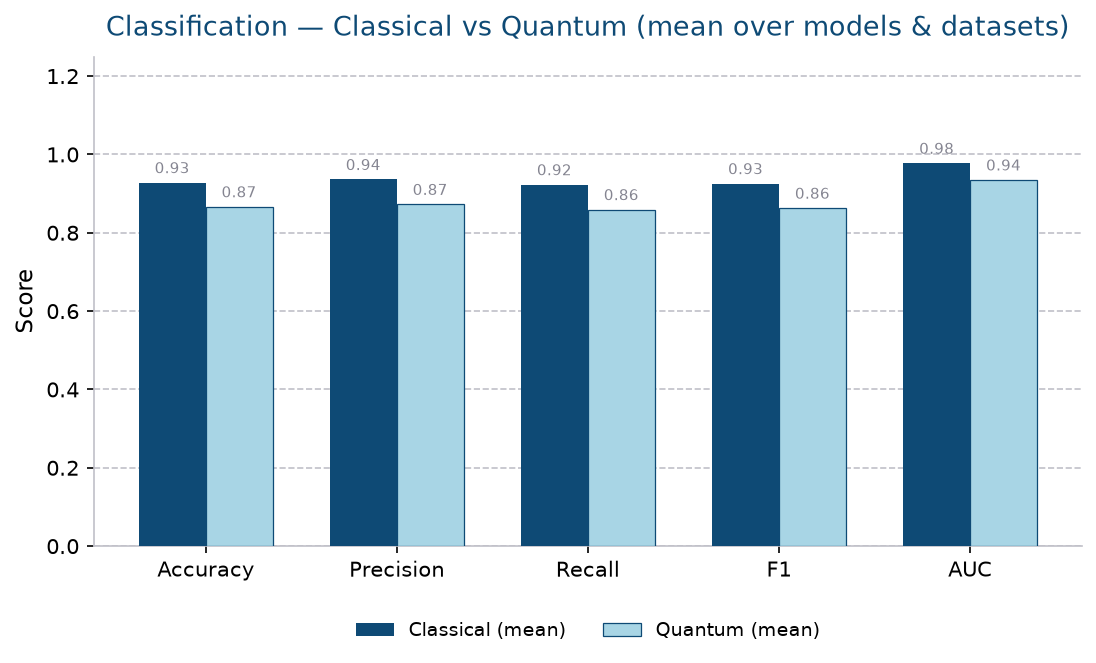
\includegraphics[width=0.88\textwidth]{cls_classical_vs_quantum.png}
\caption{Media de la familia clásica y de la cuántica sobre Iris, Bars and Stripes e Ising. El AUC cuántico no incluye el VQC, que no produce scores.}
\label{fig:cls_cq}
\end{figure}

\begin{figure}[!htbp]
\centering
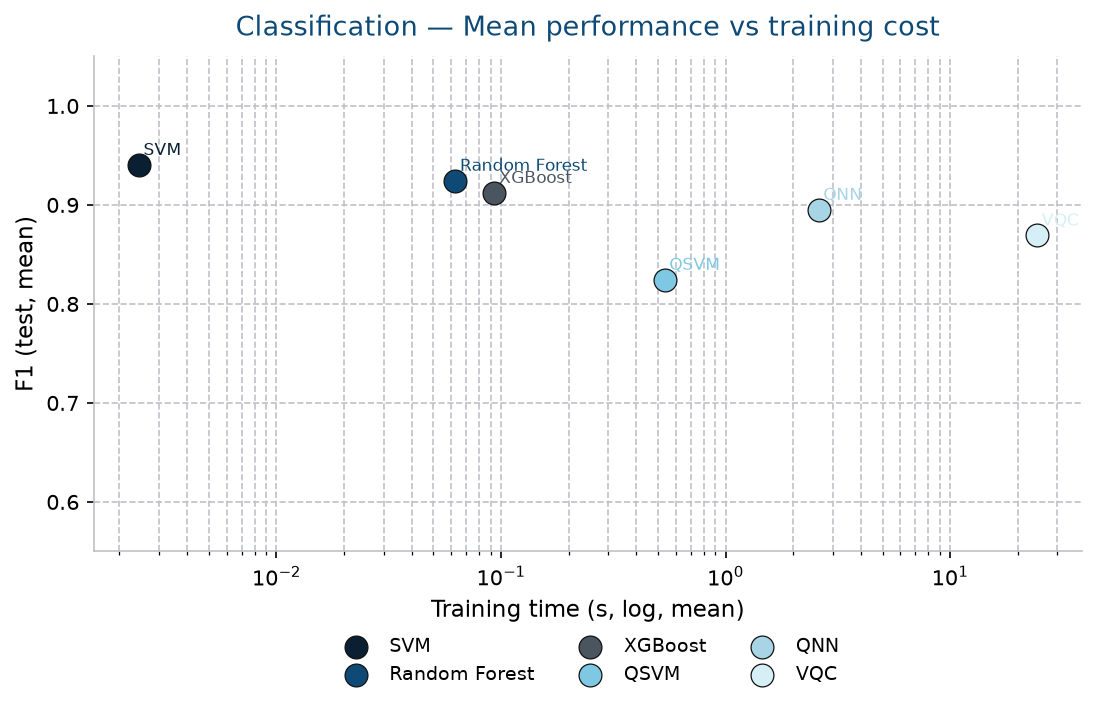
\includegraphics[width=0.82\textwidth]{cls_performance_vs_cost.png}
\caption{F1 medio de test frente al tiempo de entrenamiento (escala logarítmica). El SVM ocupa la esquina de alta calidad y bajo coste; QNN y VQC pagan el bucle variacional.}
\label{fig:cls_coste}
\end{figure}

\subsection{Iris}

Iris entra con $d=4$, sin PCA en el modelo. La proyección a dos componentes solo sirve para ver la frontera. Setosa queda aislada; las otras dos clases se solapan. La Tabla~\ref{tab:res_iris} y la Figura~\ref{fig:iris_f1} ordenan los seis clasificadores.

\begin{table}[!htbp]
\centering
\small
\resizebox{\textwidth}{!}{%
\begin{tabular}{lrrrrrr}
\toprule
\textbf{Modelo} & \textbf{Acc} & \textbf{F1} & \textbf{AUC} & \textbf{Gap} & $t_{\mathrm{train}}$ (s) & $t_{\mathrm{inf}}$ (s) \\
\midrule
SVM (RBF) & 0.967 & 0.967 & 0.998 & 0.011 & 0.002 & 0.0003 \\
Random Forest & 0.950 & 0.950 & 0.991 & 0.050 & 0.046 & 0.004 \\
XGBoost & 0.950 & 0.950 & 0.983 & 0.050 & 0.150 & 0.001 \\
QSVM & 0.733 & 0.730 & 0.883 & 0.233 & 0.072 & 0.101 \\
QNN & 0.933 & 0.933 & 0.975 & 0.022 & 1.070 & 0.006 \\
VQC & 0.950 & 0.950 & --- & $-0.006$ & 49.209 & 0.154 \\
\bottomrule
\end{tabular}}
\caption{Iris, conjunto de test. Gap $= \mathrm{Acc}_{\mathrm{train}}-\mathrm{Acc}_{\mathrm{test}}$.}
\label{tab:res_iris}
\end{table}

\begin{figure}[!htbp]
\centering
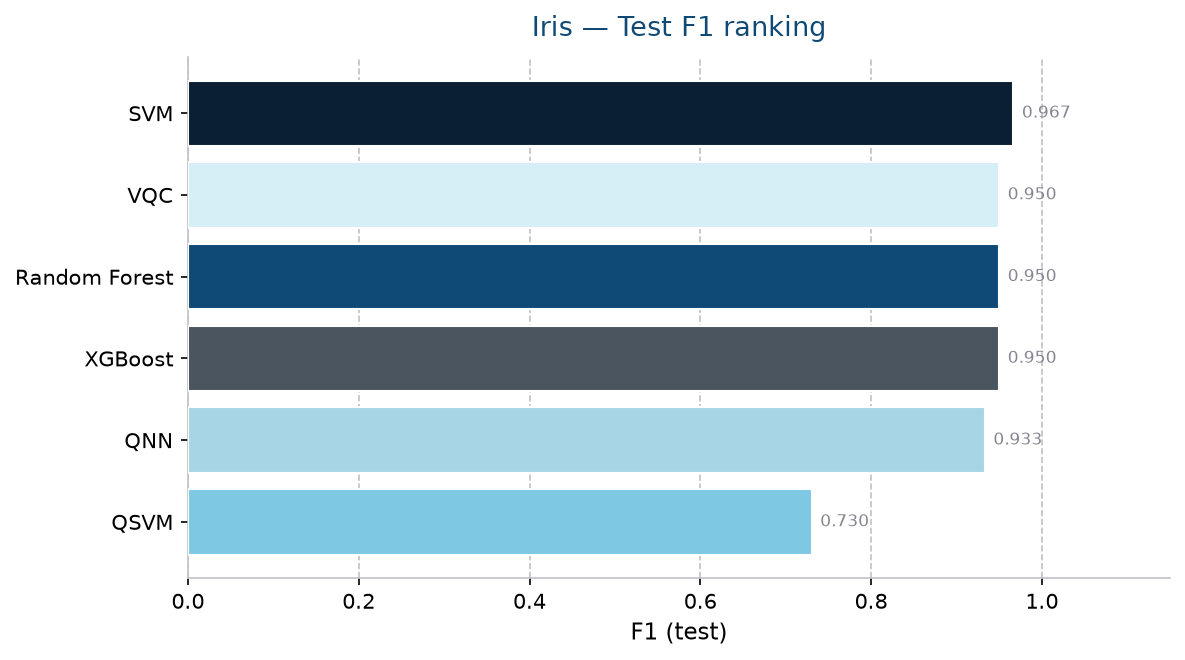
\includegraphics[width=0.72\textwidth]{iris_f1_ranking.png}
\caption{Ranking de F1 en Iris. El SVM encabeza la lista; el QSVM es el único que cae de forma clara.}
\label{fig:iris_f1}
\end{figure}

\subsubsection{SVM}

El kernel RBF corta el plano en tres bandas suaves (Figura~\ref{fig:iris_svm}). Setosa queda a un lado; el solape de las otras dos clases deja dos errores de test. F1 $0.967$, AUC $0.998$ y un gap de $0.011$ dicen que el margen generaliza. El ajuste cabe en $2\,\mathrm{ms}$. En este dataset el kernel clásico ya está alineado con la geometría: más capacidad no compra accuracy.

\begin{figure}[!htbp]
\centering
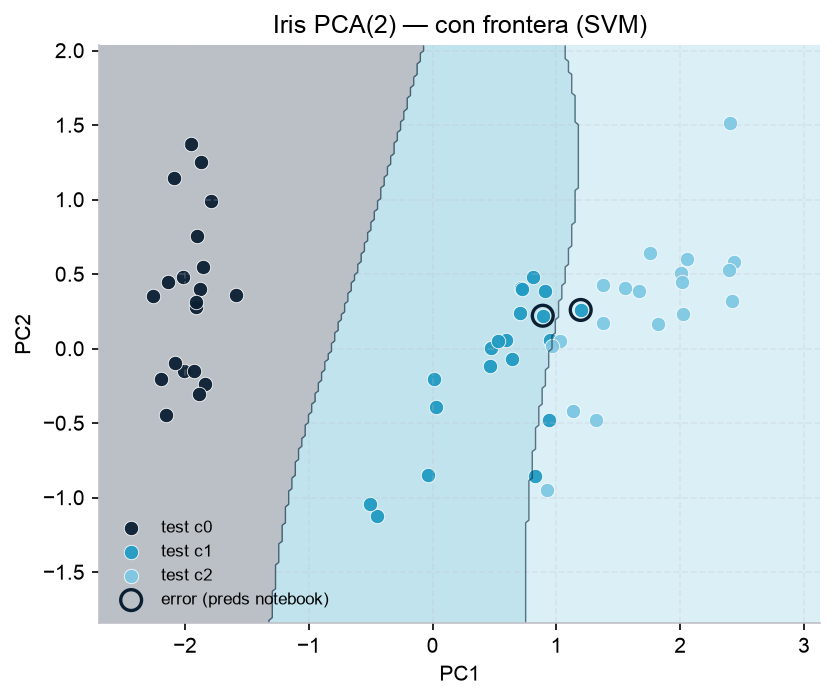
\includegraphics[width=0.72\textwidth]{svm_iris_pca_boundary.png}
\caption{Frontera del SVM en las dos primeras componentes de Iris. Los círculos marcan errores de test, concentrados en el solape de las dos clases no separables.}
\label{fig:iris_svm}
\end{figure}

\subsubsection{Random Forest}

El bosque iguala el F1 de XGBoost ($0.950$) con AUC $0.991$. El gap sube a $0.050$: algunos árboles memorizan el solape. La frontera (Figura~\ref{fig:iris_rf}) es una partición por ejes, más quebrada que la del RBF, suficiente para setosa y menos estable en la frontera de las otras dos clases. El coste sigue siendo de centésimas de segundo. Como técnica, el bagging reduce varianza, pero con $150$ muestras y tres clases el promedio de árboles no supera un kernel liso.

\begin{figure}[!htbp]
\centering
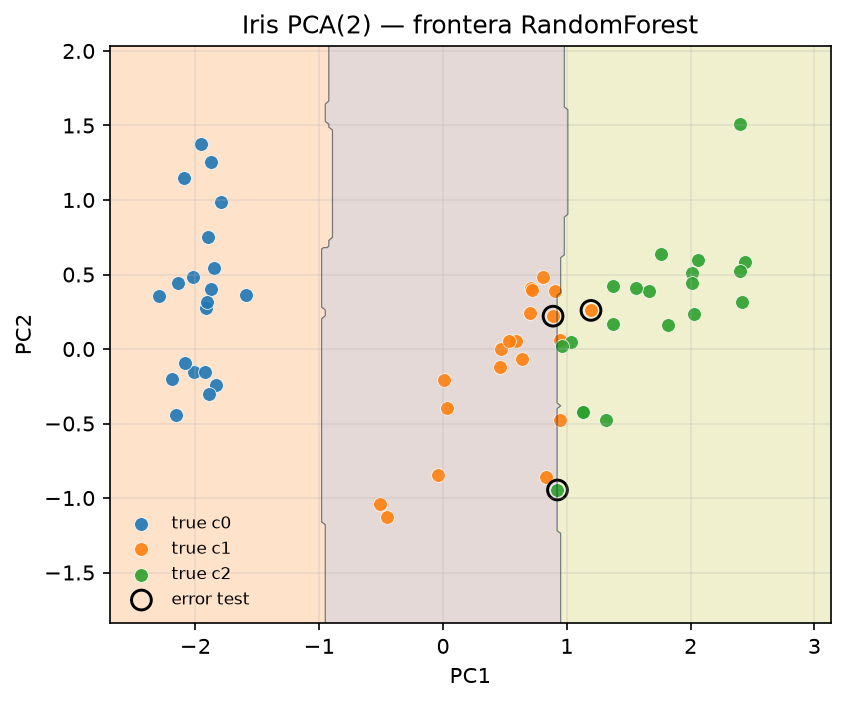
\includegraphics[width=0.72\textwidth]{rf_iris_pca_boundary.png}
\caption{Frontera del Random Forest en Iris. La partición es local; el gap de $0.050$ aparece donde las dos clases solapadas cambian de hoja.}
\label{fig:iris_rf}
\end{figure}

\subsubsection{XGBoost}

Mismas cifras de calidad que el bosque (F1 $0.950$, gap $0.050$) y AUC algo menor ($0.983$). El entrenamiento, $0.150\,\mathrm{s}$, es el más lento de los clásicos porque el boosting encadena árboles. La Figura~\ref{fig:iris_xgb} muestra una frontera por umbrales, del mismo tipo que el bosque. En Iris el gradiente boosting no explota interacciones que el RBF no cubra ya: el dato es pequeño y casi linealmente separable en la primera clase.

\begin{figure}[!htbp]
\centering
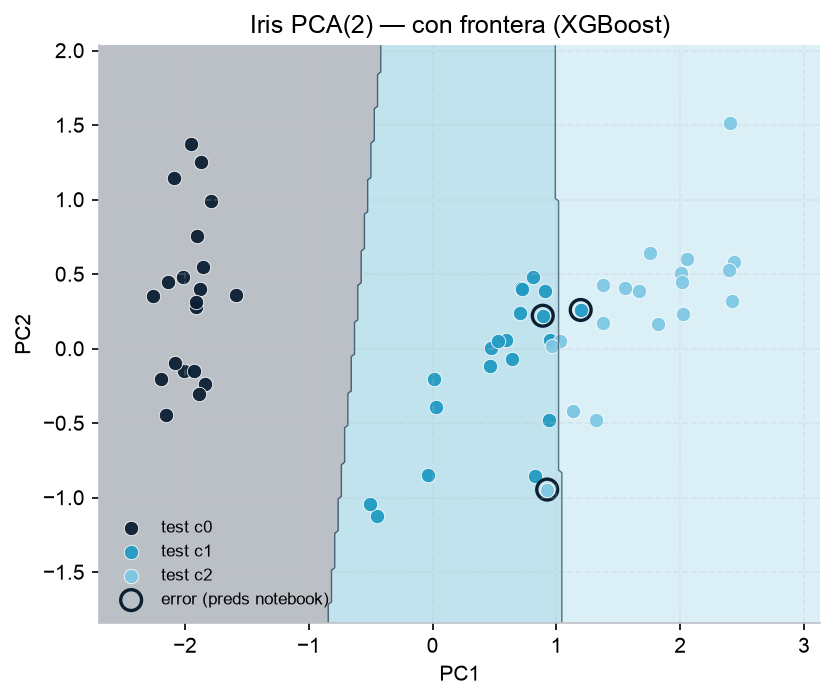
\includegraphics[width=0.72\textwidth]{xgb_iris_pca_boundary.png}
\caption{Frontera de XGBoost en Iris. La calidad empata con el bosque; el tiempo de ajuste es el mayor de la rama clásica.}
\label{fig:iris_xgb}
\end{figure}

\subsubsection{QSVM}

El mapa ZZ con kernel de fidelidad es el peor modelo del dataset: F1 $0.730$, AUC $0.883$, gap $0.233$. La Figura~\ref{fig:iris_qsvm} muestra por qué. La frontera en el plano principal está fragmentada: islas de clase dentro de regiones que el RBF deja homogéneas, y errores repartidos también en la clase que el SVM separa de un corte. El producto $Z_iZ_j$ induce un kernel sensible a correlaciones de ángulo, y el generador de etiquetas de Iris no tiene esa forma \citep{havlicek2019, huang2021}. El AUC, todavía alto respecto del accuracy, indica que el orden de los scores es más útil que el umbral duro. La inferencia ($0.101\,\mathrm{s}$) cuesta más que el ajuste: cada punto de test exige fidelidades contra el conjunto de soporte, en simulación de estado.

\begin{figure}[!htbp]
\centering
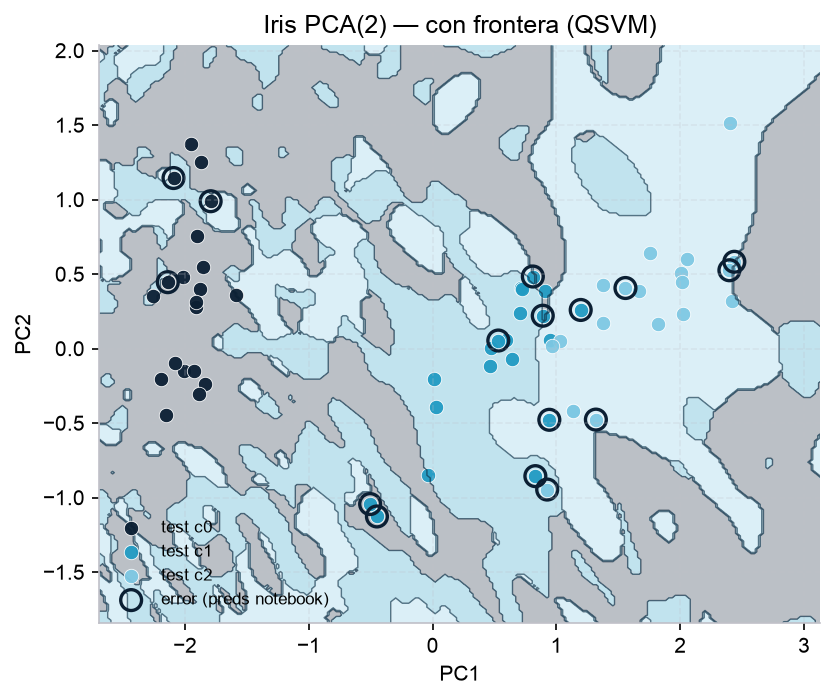
\includegraphics[width=0.72\textwidth]{qsvm_iris_pca_boundary.png}
\caption{Frontera del QSVM (mapa ZZ) en Iris. El kernel fragmenta el plano; los errores no se concentran solo en el solape.}
\label{fig:iris_qsvm}
\end{figure}

\subsubsection{QNN}

Angle embedding, capas entrelazadas y una cabeza lineal recuperan F1 $0.933$ y AUC $0.975$, a $0.033$ del SVM, con gap $0.022$. La cabeza clásica lee $\langle Z_i\rangle$ y puede suavizar una codificación angular que, por sí sola, es un producto de rotaciones. El precio está en el entrenamiento ($1.07\,\mathrm{s}$): cada época evalúa el circuito. La inferencia baja a $0.006\,\mathrm{s}$ porque la cabeza ya está ajustada. La Figura~\ref{fig:iris_qnn} muestra una frontera más continua que la del QSVM. La técnica híbrida acerca el modelo cuántico al clásico cuando el mapa no está alineado; no lo adelanta.

\begin{figure}[!htbp]
\centering
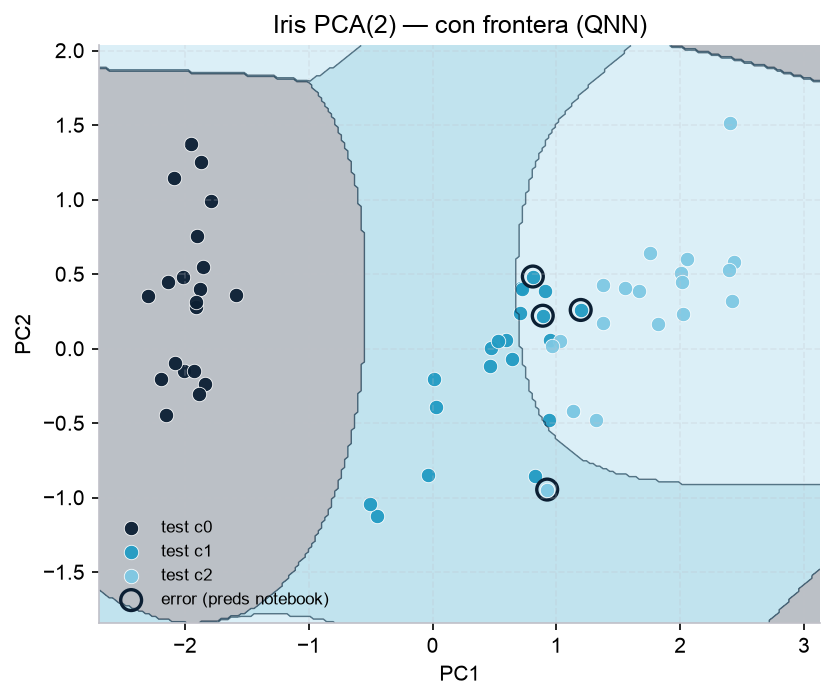
\includegraphics[width=0.72\textwidth]{qnn_iris_pca_boundary.png}
\caption{Frontera de la QNN en Iris. La cabeza lineal sobre $\langle Z_i\rangle$ produce regiones más compactas que el kernel ZZ.}
\label{fig:iris_qnn}
\end{figure}

\subsubsection{VQC}

Preparación $R_Y(x_i)$ y ansatz \texttt{Rot}+CNOT, optimizado con Nesterov, alcanzan el mismo F1 que el bosque y que XGBoost ($0.950$). El gap es ligeramente negativo ($-0.006$): el test no queda por debajo del train. La Figura~\ref{fig:iris_vqc} es una frontera variacional sobre el mismo plano. Lo que separa al VQC del SVM es el coste: $49.2\,\mathrm{s}$ de entrenamiento y $0.154\,\mathrm{s}$ de inferencia, porque cada predicción vuelve a ejecutar el circuito. Con $n=4$ y un dato que un RBF resuelve en milisegundos, el circuito variacional reproduce la calidad clásica intermedia y multiplica el tiempo \citep{cerezo2021, bowles2024}.

\begin{figure}[!htbp]
\centering
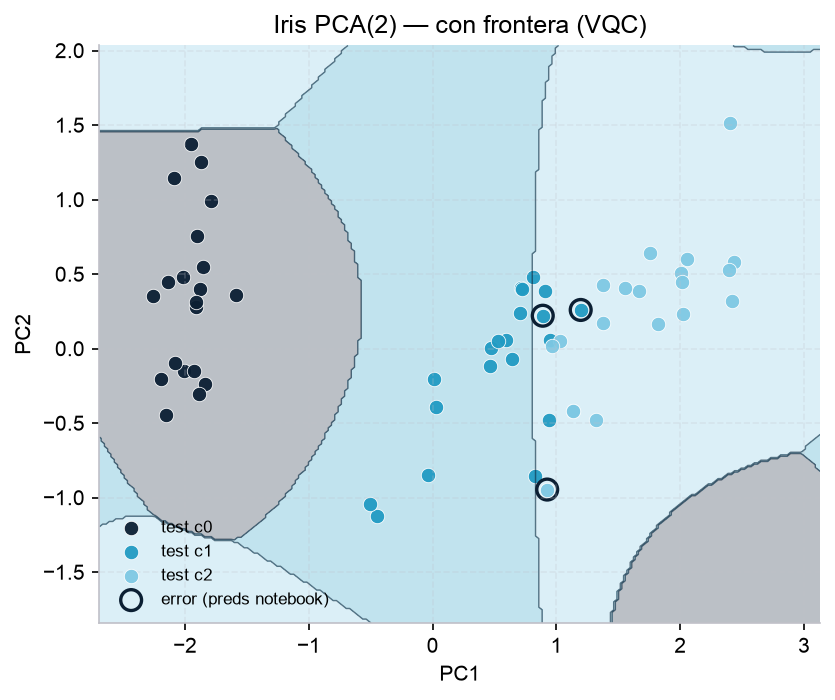
\includegraphics[width=0.72\textwidth]{vqc_iris_pca_boundary.png}
\caption{Frontera del VQC en Iris. La calidad empata con los árboles; el tiempo de entrenamiento es dos órdenes por encima del SVM.}
\label{fig:iris_vqc}
\end{figure}

\subsection{Bars and Stripes}

El patrón $4\times 4$ se aplana ($d=16$) y se reduce a cuatro componentes. En el plano de las dos primeras las dos clases se mezclan, así que ninguna frontera suave es suficiente. La Tabla~\ref{tab:res_bs} es el dataset donde la rama cuántica queda más lejos del mejor clásico, salvo la QNN en AUC.

\begin{table}[!htbp]
\centering
\small
\resizebox{\textwidth}{!}{%
\begin{tabular}{lrrrrrr}
\toprule
\textbf{Modelo} & \textbf{Acc} & \textbf{F1} & \textbf{AUC} & \textbf{Gap} & $t_{\mathrm{train}}$ (s) & $t_{\mathrm{inf}}$ (s) \\
\midrule
SVM (RBF) & 0.871 & 0.870 & 0.936 & 0.021 & 0.003 & 0.007 \\
Random Forest & 0.854 & 0.854 & 0.943 & 0.146 & 0.078 & 0.006 \\
XGBoost & 0.850 & 0.849 & 0.953 & 0.067 & 0.074 & 0.001 \\
QSVM & 0.758 & 0.758 & 0.822 & 0.110 & 1.458 & 1.538 \\
QNN & 0.817 & 0.815 & 0.936 & $-0.006$ & 5.614 & 0.006 \\
VQC & 0.696 & 0.688 & --- & 0.014 & 12.432 & 1.872 \\
\bottomrule
\end{tabular}}
\caption{Bars and Stripes, conjunto de test.}
\label{tab:res_bs}
\end{table}

\begin{figure}[!htbp]
\centering
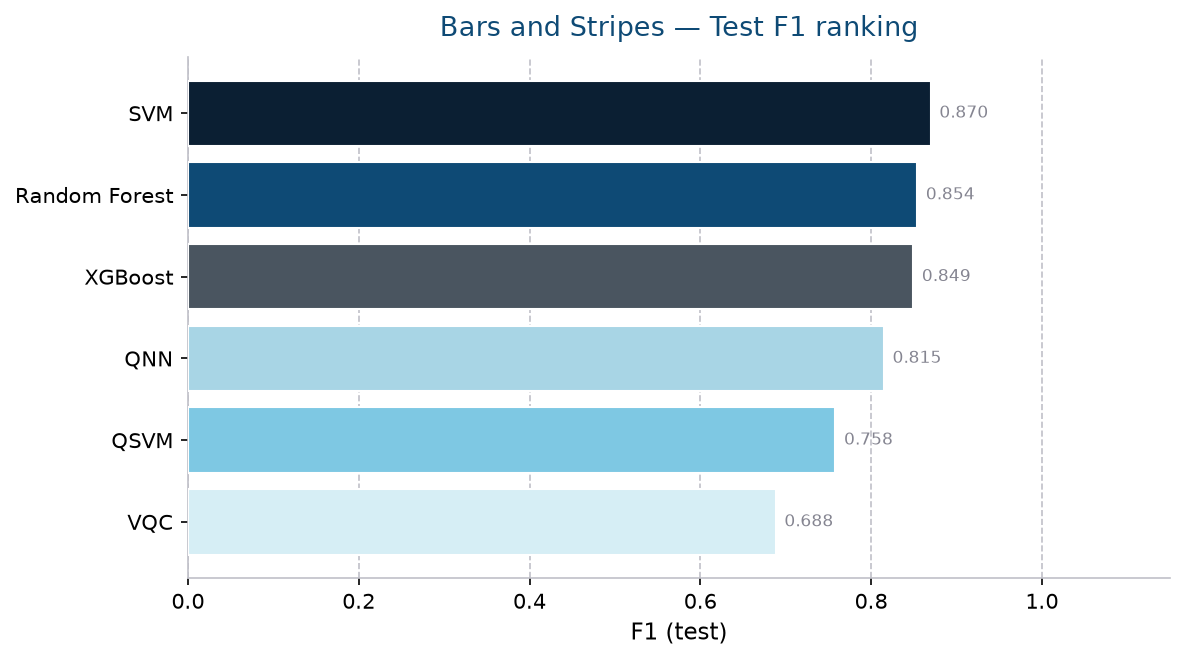
\includegraphics[width=0.72\textwidth]{bs_f1_ranking.png}
\caption{Ranking de F1 en Bars and Stripes. El SVM lidera; el VQC cierra la lista.}
\label{fig:bs_f1}
\end{figure}

\begin{figure}[!htbp]
\centering
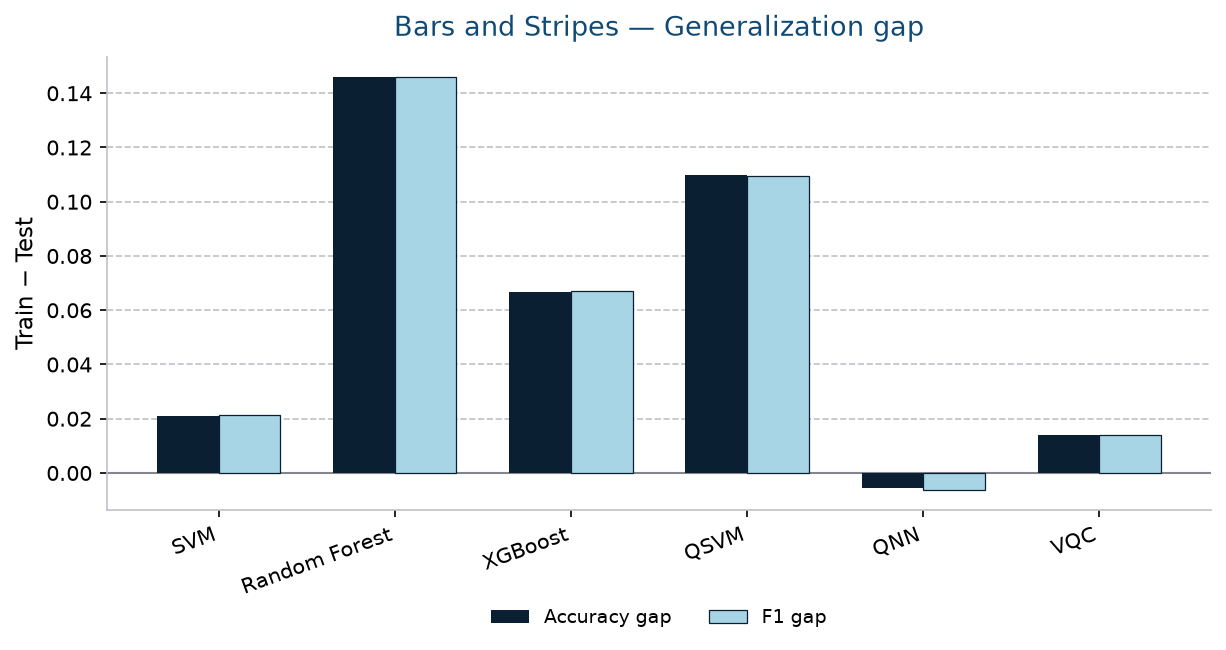
\includegraphics[width=0.78\textwidth]{bs_generalization_gap.png}
\caption{Gap de generalización en Bars and Stripes. El Random Forest es el que más se separa entre train y test.}
\label{fig:bs_gap}
\end{figure}

\subsubsection{SVM}

F1 $0.870$ y gap $0.021$: el RBF sigue siendo el mejor compromiso. El AUC $0.936$ muestra que, aunque el plano está mezclado, el kernel ordena razonablemente las dos clases. La Figura~\ref{fig:bs_svm} coloca la frontera sobre esa nube. Con $d$ reducido a 4, el RBF opera en el mismo presupuesto de coordenadas que los circuitos y aun así generaliza mejor que ellos. El tiempo total permanece por debajo de la centésima de segundo.

\begin{figure}[!htbp]
\centering
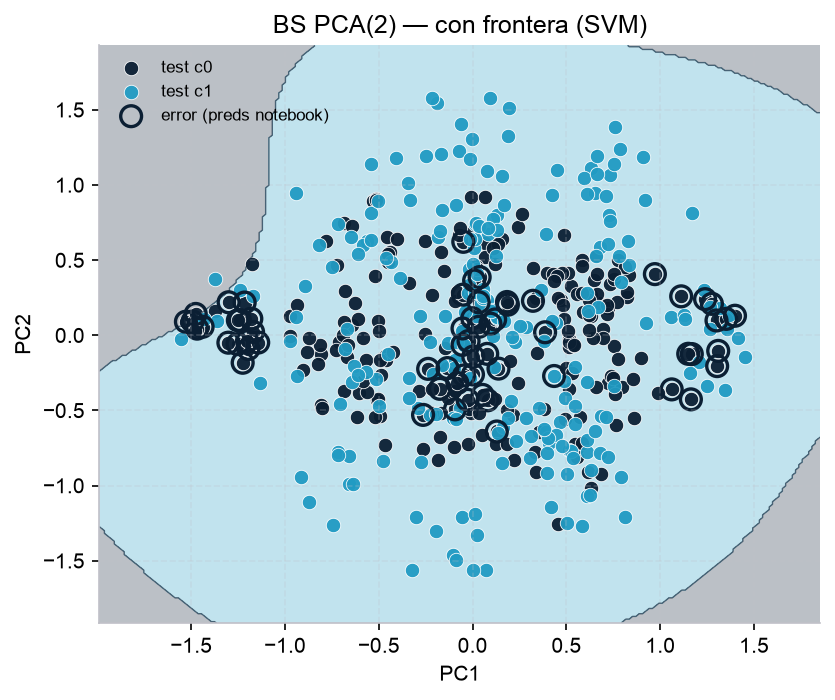
\includegraphics[width=0.72\textwidth]{svm_bs_pca_boundary.png}
\caption{Frontera del SVM en Bars and Stripes. El plano mezcla las clases; el margen RBF es el que menos errores acumula.}
\label{fig:bs_svm}
\end{figure}

\subsubsection{Random Forest}

F1 $0.854$, AUC $0.943$, gap $0.146$. El bosque acierta en train y pierde en test: las reglas que aíslan barras y franjas en las hojas no sobreviven al $40\%$ de test. La Figura~\ref{fig:bs_rf} es una partición fina de una nube sin margen. En un dato de patrones binarios comprimidos por PCA, el bagging memoriza combinaciones de componentes que no son estables. Es el caso claro en que accuracy de train no es la métrica de la comparación.

\begin{figure}[!htbp]
\centering
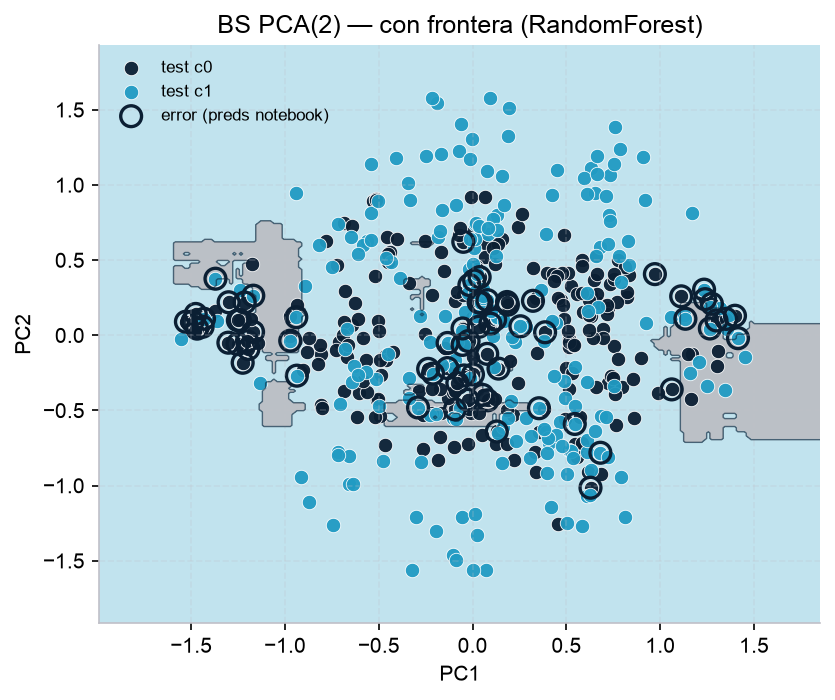
\includegraphics[width=0.72\textwidth]{rf_bs_pca_boundary.png}
\caption{Frontera del Random Forest en Bars and Stripes. La partición ajusta el train; el gap de $0.146$ mide lo que no se sostiene en test.}
\label{fig:bs_rf}
\end{figure}

\subsubsection{XGBoost}

F1 $0.849$, el AUC más alto del dataset ($0.953$) y un gap de $0.067$, menos de la mitad que el bosque. El boosting regulariza la secuencia de árboles y ordena mejor las probabilidades, aunque la etiqueta dura quede un punto por debajo del SVM. La Figura~\ref{fig:bs_xgb} muestra esa frontera. La técnica aporta calibración (el AUC) más que accuracy: para un ranking de patrones, XGBoost es el clásico a mirar; para la etiqueta, el RBF sigue delante.

\begin{figure}[!htbp]
\centering
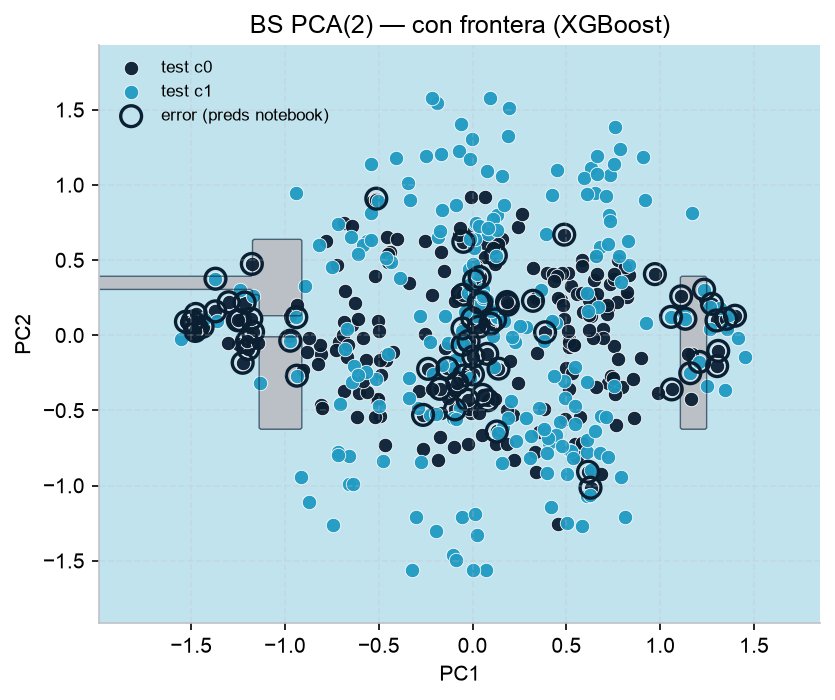
\includegraphics[width=0.72\textwidth]{xgb_bs_pca_boundary.png}
\caption{Frontera de XGBoost en Bars and Stripes. El F1 queda justo bajo el SVM; el AUC es el más alto de la tabla.}
\label{fig:bs_xgb}
\end{figure}

\subsubsection{QSVM}

F1 $0.758$, AUC $0.822$, gap $0.110$. El mapa ZZ no encuentra en las cuatro componentes una correlación que separe barras de franjas mejor que un RBF. El coste cambia de escala: $1.46\,\mathrm{s}$ de ajuste y $1.54\,\mathrm{s}$ de inferencia, porque la matriz de fidelidad crece con el producto de tamaños de train y test y cada entrada es un solape de estados. La Figura~\ref{fig:bs_qsvm} es la frontera inducida por ese kernel. En un dataset convencional, sin generador cuántico de las etiquetas, el feature map ZZ es una hipótesis inductiva cara y peor alineada \citep{huang2021, schuld2021}.

\begin{figure}[!htbp]
\centering
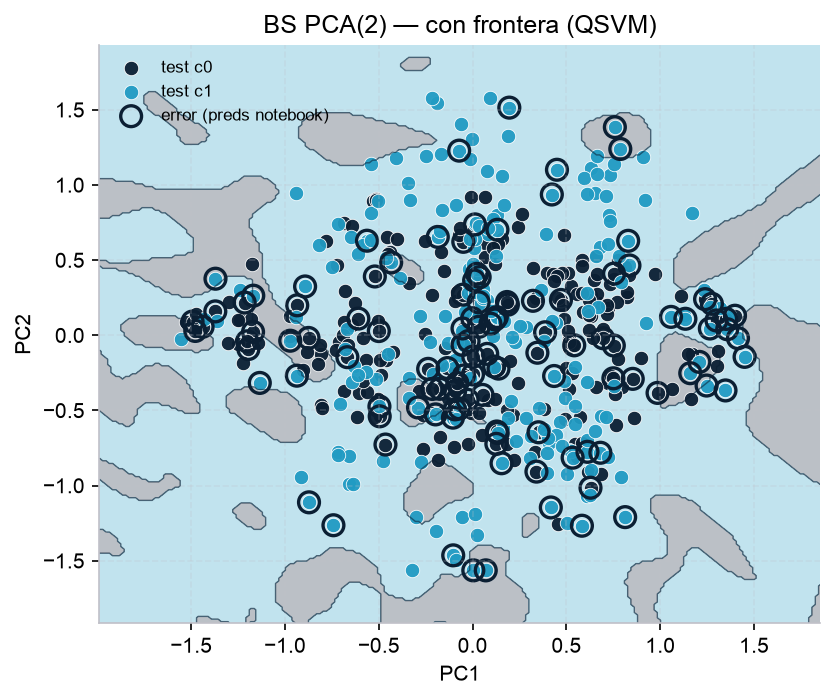
\includegraphics[width=0.72\textwidth]{qsvm_bs_pca_boundary.png}
\caption{Frontera del QSVM en Bars and Stripes. El kernel de fidelidad no ordena la nube mejor que el RBF y multiplica el tiempo de inferencia.}
\label{fig:bs_qsvm}
\end{figure}

\subsubsection{QNN}

Es el mejor modelo cuántico del dataset: F1 $0.815$, AUC $0.936$ (el mismo que el SVM) y gap ligeramente negativo. La etiqueta dura queda $0.055$ por debajo del SVM; el orden de los scores no. Angle embedding más entrelazamiento entrenable y una cabeza lineal leen una geometría que el kernel ZZ no linealiza igual. El entrenamiento dura $5.61\,\mathrm{s}$; la inferencia, $0.006\,\mathrm{s}$. La Figura~\ref{fig:bs_qnn} muestra la frontera. La discusión de técnica es la de un modelo híbrido: el circuito propone features $\langle Z_i\rangle$ y la cabeza clásica clasifica. En Bars and Stripes esa división acerca el AUC al mejor clásico y deja la accuracy todavía por debajo.

\begin{figure}[!htbp]
\centering
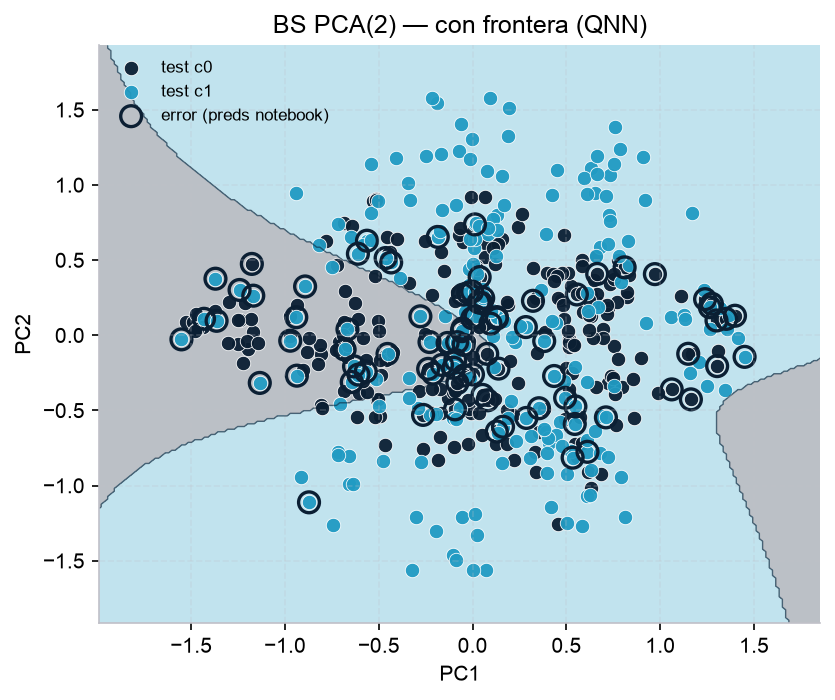
\includegraphics[width=0.72\textwidth]{qnn_bs_pca_boundary.png}
\caption{Frontera de la QNN en Bars and Stripes. El AUC empata con el SVM; la etiqueta dura no.}
\label{fig:bs_qnn}
\end{figure}

\subsubsection{VQC}

F1 $0.688$, el mínimo del corpus de clasificación, con $12.4\,\mathrm{s}$ de entrenamiento y $1.87\,\mathrm{s}$ de inferencia. La Figura~\ref{fig:bs_vqc} muestra un corte simple sobre la nube mezclada: el ansatz $R_Y$ más \texttt{Rot}+CNOT, leído por $\langle Z\rangle$, no tiene grados de libertad para una frontera que siga el solape. El mismo circuito en Iris, donde una clase está separada, empataba con los árboles. Aquí la hipótesis del ansatz es demasiado rígida para el dato. Subir capas aumentaría el coste de simulación sin garantía de alinear el mapa con las barras \citep{cerezo2021}.

\begin{figure}[!htbp]
\centering
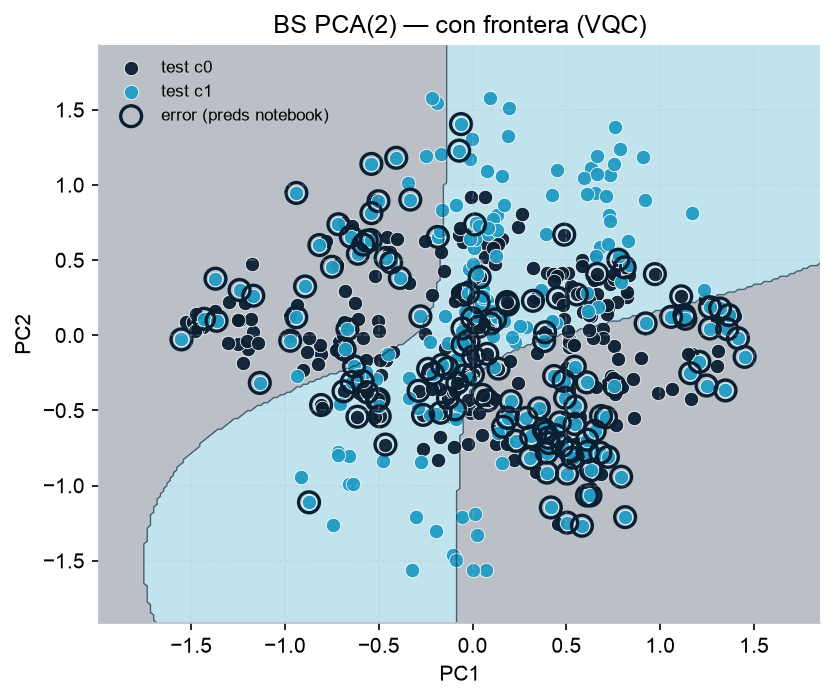
\includegraphics[width=0.72\textwidth]{vqc_bs_pca_boundary.png}
\caption{Frontera del VQC en Bars and Stripes. El corte deja la región de solape llena de errores de test.}
\label{fig:bs_vqc}
\end{figure}

\subsection{Ising}

Las features son amplitudes del estado fundamental de una cadena de cuatro espines. La etiqueta es la fase, $y=\mathbf{1}[h>|J|]$, y $h$ no entra como variable. Tras la PCA el plano se organiza en dos ramas. Es el único dataset en el que un modelo cuántico empata con el mejor clásico (Tabla~\ref{tab:res_ising}).

\begin{table}[!htbp]
\centering
\small
\resizebox{\textwidth}{!}{%
\begin{tabular}{lrrrrrr}
\toprule
\textbf{Modelo} & \textbf{Acc} & \textbf{F1} & \textbf{AUC} & \textbf{Gap} & $t_{\mathrm{train}}$ (s) & $t_{\mathrm{inf}}$ (s) \\
\midrule
SVM (RBF) & 0.988 & 0.985 & 1.000 & 0.013 & 0.001 & 0.0002 \\
Random Forest & 0.975 & 0.969 & 1.000 & 0.025 & 0.062 & 0.004 \\
XGBoost & 0.950 & 0.937 & 0.996 & 0.050 & 0.012 & 0.0005 \\
QSVM & 0.988 & 0.985 & 1.000 & 0.013 & 0.153 & 0.206 \\
QNN & 0.950 & 0.937 & 0.996 & 0.017 & 2.843 & 0.006 \\
VQC & 0.975 & 0.969 & --- & 0.000 & 18.231 & 0.332 \\
\bottomrule
\end{tabular}}
\caption{Ising, conjunto de test. Recall macro del SVM y del QSVM: $0.979$.}
\label{tab:res_ising}
\end{table}

\begin{figure}[!htbp]
\centering
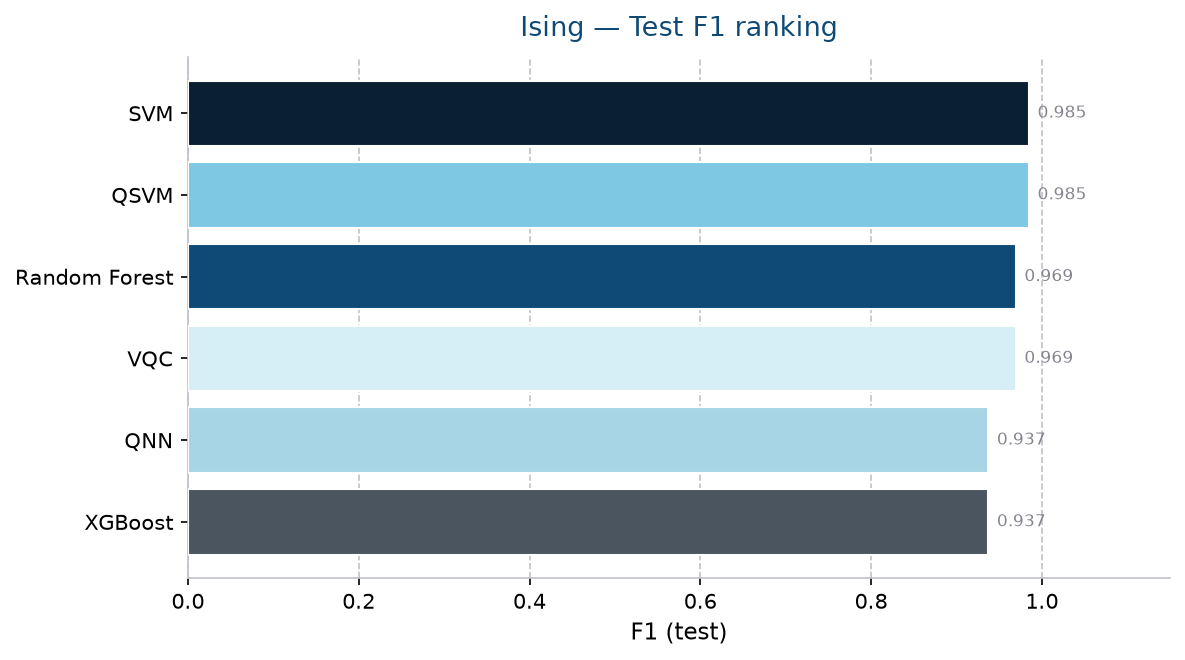
\includegraphics[width=0.72\textwidth]{ising_f1_ranking.png}
\caption{Ranking de F1 en Ising. SVM y QSVM comparten el primer puesto.}
\label{fig:ising_f1}
\end{figure}

\subsubsection{SVM}

F1 $0.985$, AUC $1.000$, gap $0.013$, en alrededor de un milisegundo. El recall macro ($0.979$) queda un punto bajo el accuracy: la clase minoritaria de fase concentra el error residual. La Figura~\ref{fig:ising_svm} sigue las dos ramas del plano. El RBF no necesita saber que el vector viene de un estado cuántico; la geometría tras la PCA ya es separable. Por eso el empate posterior del QSVM no es, por sí solo, una ventaja operativa: el mismo F1 llega antes por el kernel clásico.

\begin{figure}[!htbp]
\centering
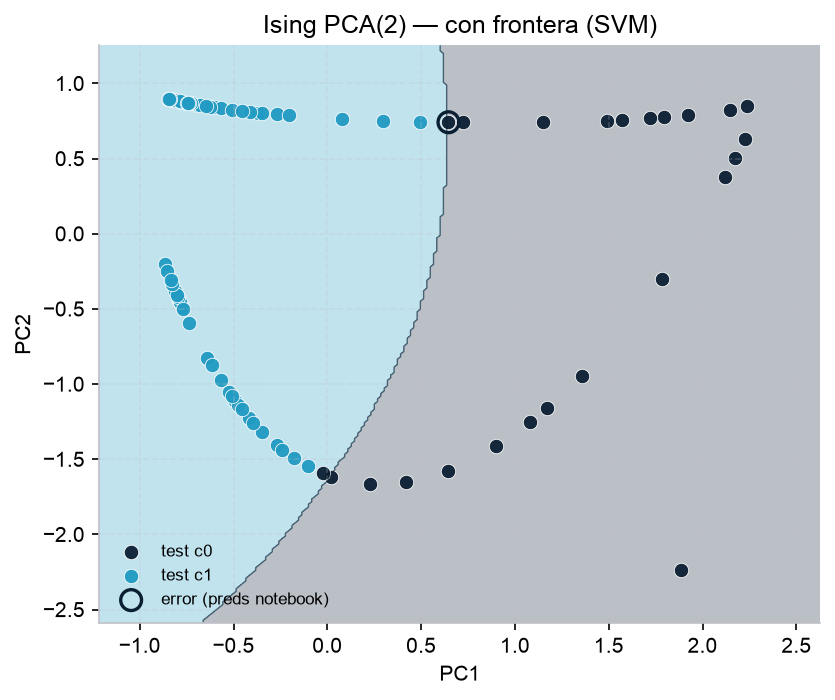
\includegraphics[width=0.72\textwidth]{svm_ising_pca_boundary.png}
\caption{Frontera del SVM en Ising. Las dos ramas de fase quedan separadas; el error residual es de una clase.}
\label{fig:ising_svm}
\end{figure}

\subsubsection{Random Forest}

F1 $0.969$ y AUC $1.000$, con gap $0.025$. El bosque ordena las fases tan bien como el SVM en AUC y pierde algo de F1 en la etiqueta dura. La Figura~\ref{fig:ising_rf} corta las ramas con umbrales. Con componentes principales tan estructuradas, un árbol encuentra el corte; el bagging no añade mucho sobre un solo margen. El tiempo ($0.062\,\mathrm{s}$) sigue siendo inferior al de cualquier circuito.

\begin{figure}[!htbp]
\centering
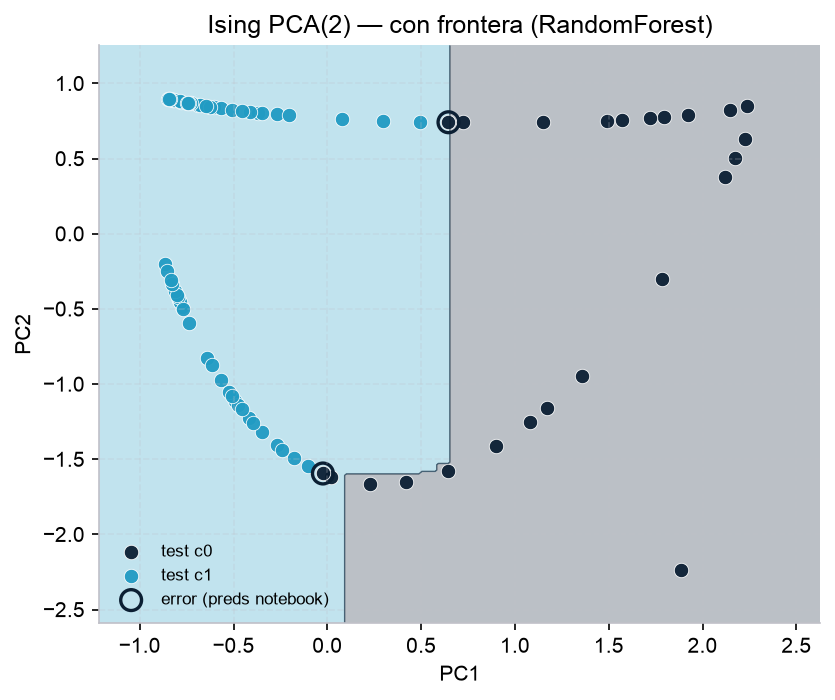
\includegraphics[width=0.72\textwidth]{rf_ising_pca_boundary.png}
\caption{Frontera del Random Forest en Ising. AUC perfecto y F1 un punto por debajo del SVM.}
\label{fig:ising_rf}
\end{figure}

\subsubsection{XGBoost}

F1 $0.937$, recall macro $0.917$, AUC $0.996$, gap $0.050$. Es el clásico que más se deja la fase minoritaria. El boosting, con este tamaño de muestra, ajusta de más el corte entre ramas (Figura~\ref{fig:ising_xgb}). El dato premia un margen global; una secuencia de árboles cortos no es esa hipótesis. Aun así el ajuste dura $0.012\,\mathrm{s}$.

\begin{figure}[!htbp]
\centering
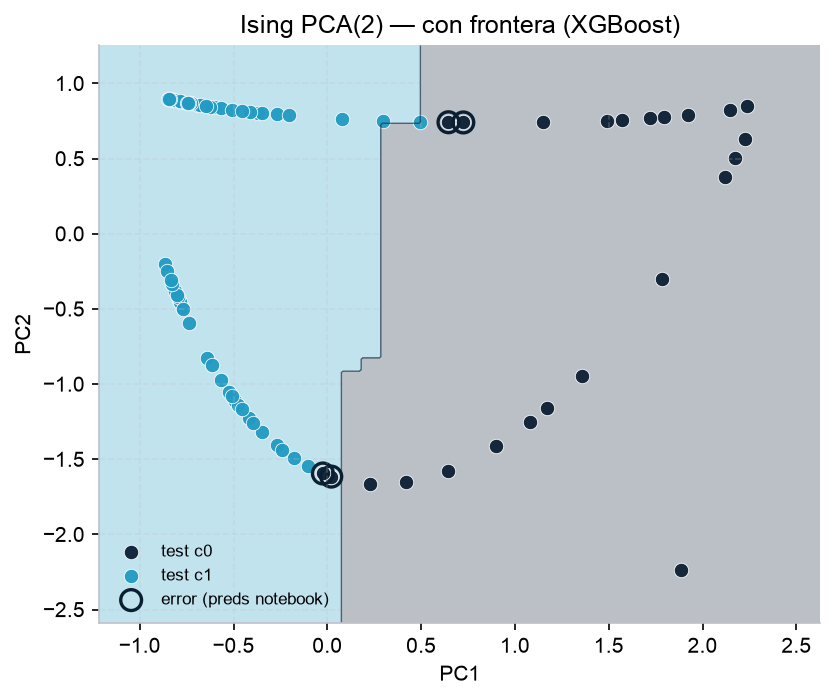
\includegraphics[width=0.72\textwidth]{xgb_ising_pca_boundary.png}
\caption{Frontera de XGBoost en Ising. El recall macro cae a $0.917$: la fase menos representada concentra los errores.}
\label{fig:ising_xgb}
\end{figure}

\subsubsection{QSVM}

Empata con el SVM en Acc $0.988$, F1 $0.985$, AUC $1.000$ y gap $0.013$. La Figura~\ref{fig:ising_qsvm} sigue las dos ramas y deja un error visible en la zona de transición. Aquí el mapa ZZ sí está cerca del generador: las features son amplitudes de un estado de Ising y la etiqueta es la fase de ese mismo Hamiltoniano \citep{huang2021, havlicek2019}. El empate de calidad no arrastra al tiempo. El ajuste dura $0.153\,\mathrm{s}$ y la inferencia $0.206\,\mathrm{s}$, frente a $0.001\,\mathrm{s}$ del SVM. La discusión queda en la alineación dato--mapa: cuando el kernel cuántico está en el espacio correcto, recupera al clásico; la simulación del solape sigue costando más que evaluar un RBF.

\begin{figure}[!htbp]
\centering
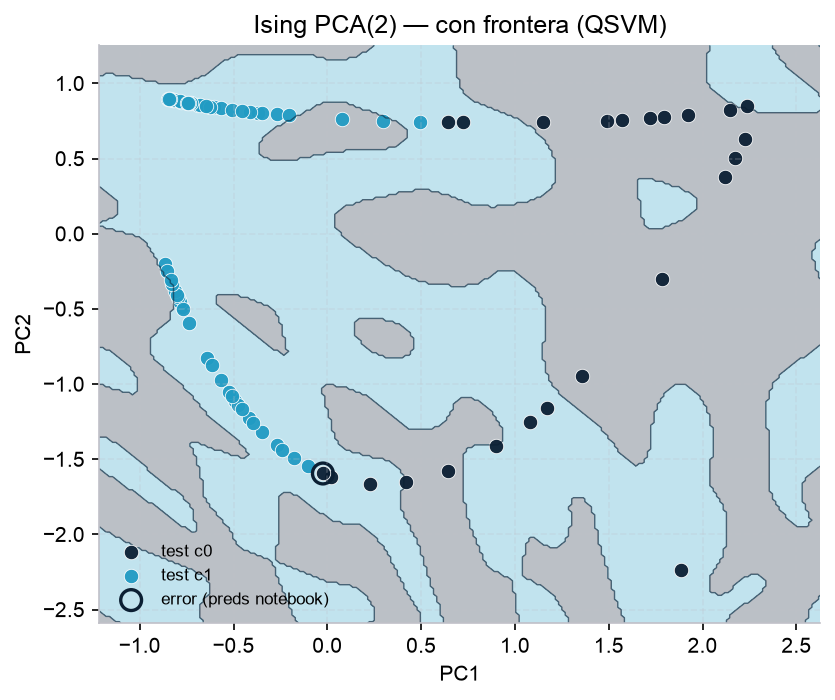
\includegraphics[width=0.72\textwidth]{qsvm_ising_pca_boundary.png}
\caption{Frontera del QSVM en Ising. El mapa ZZ separa las ramas de fase; queda un error junto a la transición.}
\label{fig:ising_qsvm}
\end{figure}

\subsubsection{QNN}

F1 $0.937$ y AUC $0.996$, las mismas cifras que XGBoost, con gap menor ($0.017$). La cabeza lineal sobre angle embedding no aprovecha la estructura de fase mejor que un boosting corto, y el entrenamiento sube a $2.84\,\mathrm{s}$. La Figura~\ref{fig:ising_qnn} muestra la frontera. En un dato donde el kernel ZZ ya empata con el RBF, cambiar a un embedding angular separable y entrenar capas es una hipótesis más débil: se pierde la interacción $Z_iZ_j$ que justificaba el mapa.

\begin{figure}[!htbp]
\centering
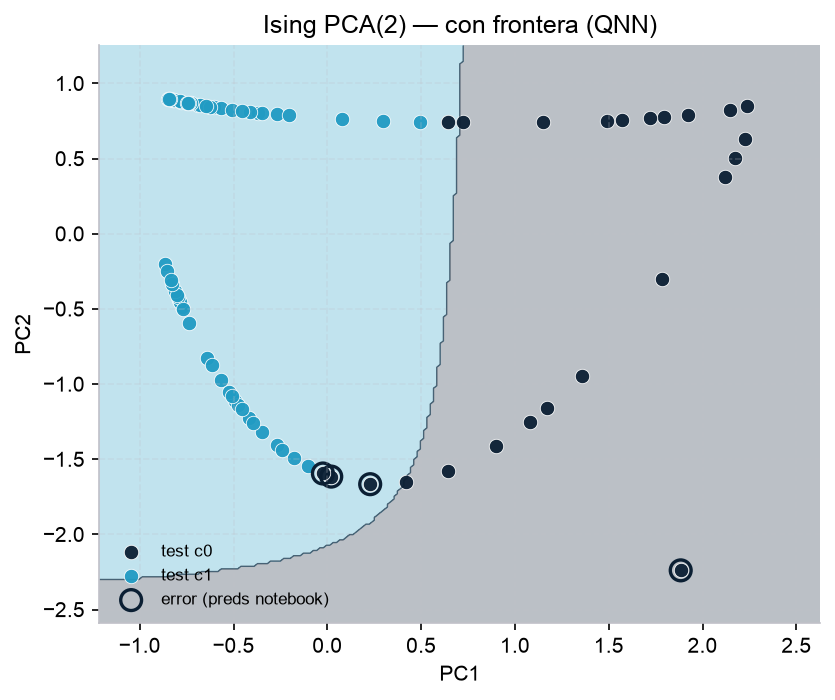
\includegraphics[width=0.72\textwidth]{qnn_ising_pca_boundary.png}
\caption{Frontera de la QNN en Ising. La calidad queda en el nivel de XGBoost, por debajo del par SVM--QSVM.}
\label{fig:ising_qnn}
\end{figure}

\subsubsection{VQC}

F1 $0.969$, el mismo que el Random Forest, gap $0.000$ y $18.2\,\mathrm{s}$ de entrenamiento. La preparación $R_Y$ más el ansatz variacional cabe en la geometría de dos ramas (Figura~\ref{fig:ising_vqc}) sin el sobreajuste de XGBoost. No alcanza el empate SVM--QSVM. Cada predicción reejecuta el circuito ($0.332\,\mathrm{s}$). Frente al QSVM, el VQC no usa el kernel alineado con el Hamiltoniano; frente al SVM, repite una calidad intermedia a un coste de simulación que en este tamaño no se justifica \citep{bowles2024}.

\begin{figure}[!htbp]
\centering
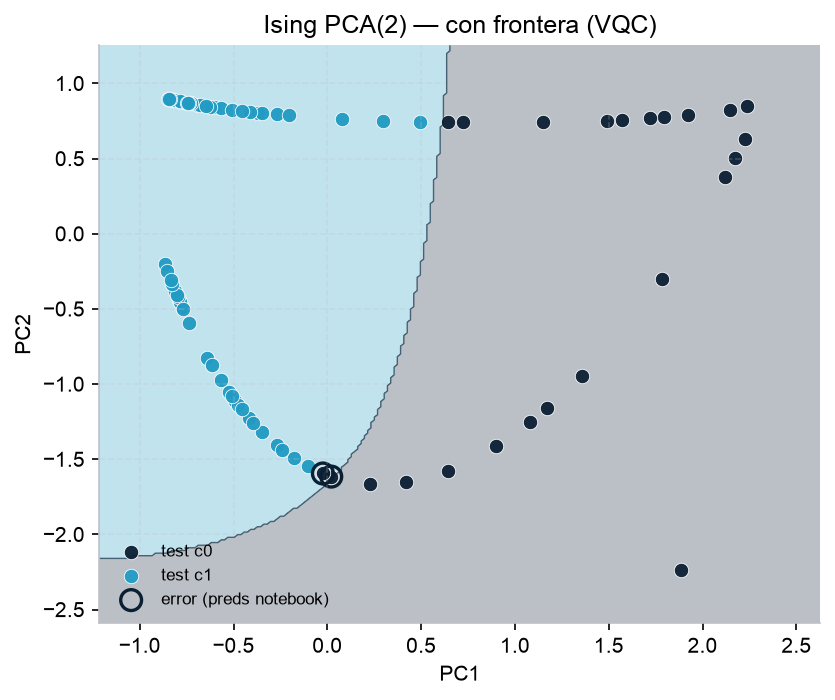
\includegraphics[width=0.72\textwidth]{vqc_ising_pca_boundary.png}
\caption{Frontera del VQC en Ising. Gap nulo y F1 de bosque, con el mayor tiempo de inferencia de la tabla tras el QSVM.}
\label{fig:ising_vqc}
\end{figure}

\subsection{Lectura de la familia}

Tres técnicas, tres resultados. El kernel RBF es el mejor o está empatado en los tres datasets y es el más barato. Los árboles se acercan cuando la geometría es simple (Iris, Ising) y generalizan peor cuando la nube está mezclada (Bars and Stripes, gap del bosque $0.146$). El mapa ZZ solo empata con el RBF en Ising, donde las features ya son un estado de un Hamiltoniano y la etiqueta es su fase; en Iris fragmenta la frontera y en Bars and Stripes paga segundos de fidelidad por un F1 inferior \citep{huang2021}. La QNN híbrida es el cuántico más estable fuera de Ising: su AUC en Bars and Stripes iguala al SVM, porque la cabeza clásica clasifica $\langle Z_i\rangle$. El VQC reproduce la calidad de los árboles en Iris e Ising y cae en Bars and Stripes, siempre con el mayor tiempo de entrenamiento. En simulación de $n=4$, la comparación cuantitativa no muestra una región en la que el circuito mejore al RBF en F1 y en tiempo a la vez \citep{bowles2024}.

\section{Optimización}

Las instancias tienen óptimo conocido y caben en enumeración: TSP con coste $C^\star=16$, MDS con $C^\star=2$, MaxCut con $C^\star=8$. La Figura~\ref{fig:opt_success} sitúa el success rate medio frente al tiempo. El detalle, y las dos excepciones (greedy en MDS, QAOA en MDS, SA en TSP), está en las tablas de cada problema. En este tamaño, alcanzar $C^\star$ es lo esperado de un método exacto; lo que distingue a los solvers es el camino y el wall-clock \citep{lubinski2024, lucas2014}.

\begin{figure}[!htbp]
\centering
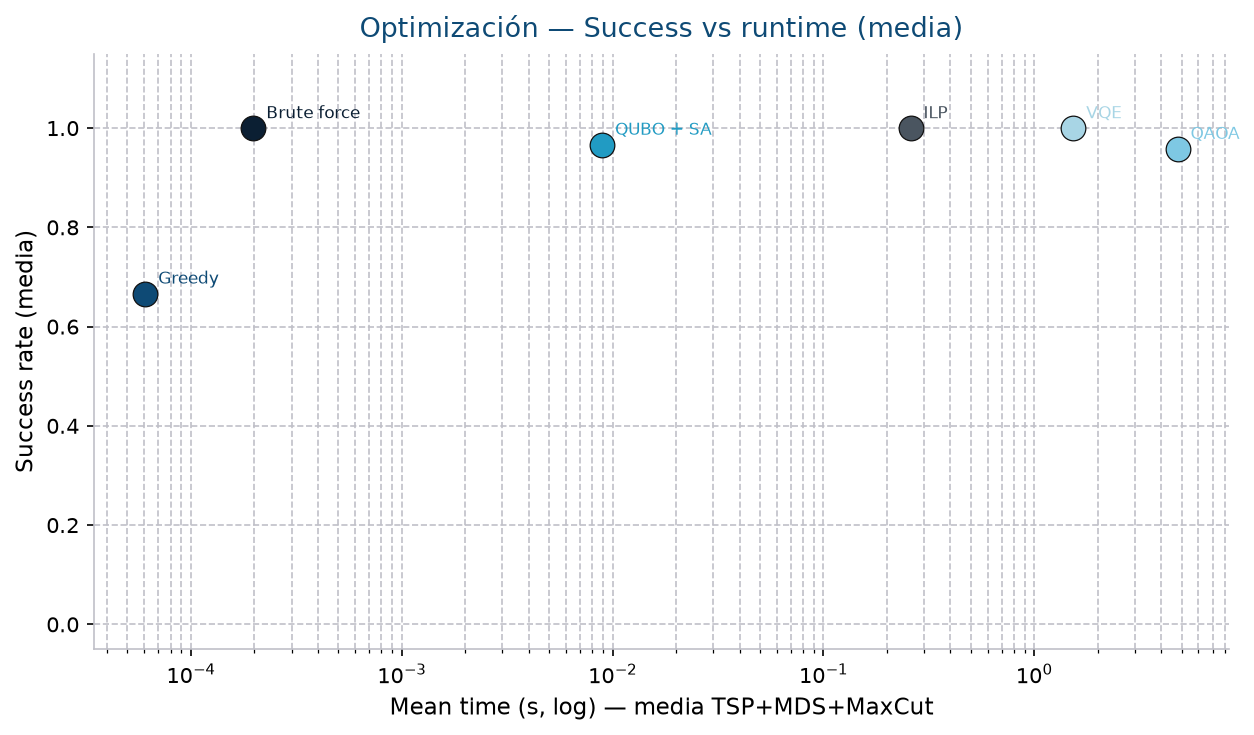
\includegraphics[width=0.82\textwidth]{opt_success_vs_runtime_mean.png}
\caption{Success rate medio frente al tiempo medio. La fuerza bruta es exacta y barata en estas instancias; QAOA y VQE se sitúan en segundos de simulación.}
\label{fig:opt_success}
\end{figure}

\subsection{TSP}

Grafo completo de 5 nodos. El óptimo por enumeración es $16$. La Tabla~\ref{tab:res_tsp} y la Figura~\ref{fig:tsp_success} resumen los seis solvers.

\begin{table}[!htbp]
\centering
\small
\resizebox{\textwidth}{!}{%
\begin{tabular}{lrrrrrr}
\toprule
\textbf{Solver} & \textbf{Éxito} & $C$ medio & $C$ mejor & \textbf{Gap} & \textbf{Gap rel.} & $t$ (s) \\
\midrule
Fuerza bruta & 1.00 & 16.0 & 16 & 0.00 & 0.000 & 0.0009 \\
Greedy & 1.00 & 16.0 & 16 & 0.00 & 0.000 & 0.0005 \\
ILP & 1.00 & 16.0 & 16 & 0.00 & 0.000 & 1.277 \\
QUBO + SA & 0.90 & 16.3 & 16 & 0.30 & 0.019 & 0.017 \\
QAOA & 1.00 & 16.0 & 16 & 0.00 & 0.000 & 1.059 \\
VQE & 1.00 & 16.0 & 16 & 0.00 & 0.000 & 1.909 \\
\bottomrule
\end{tabular}}
\caption{TSP. $C^\star=16$. El SA promedia semillas; el resto alcanza el óptimo en las ejecuciones reportadas.}
\label{tab:res_tsp}
\end{table}

\begin{figure}[!htbp]
\centering
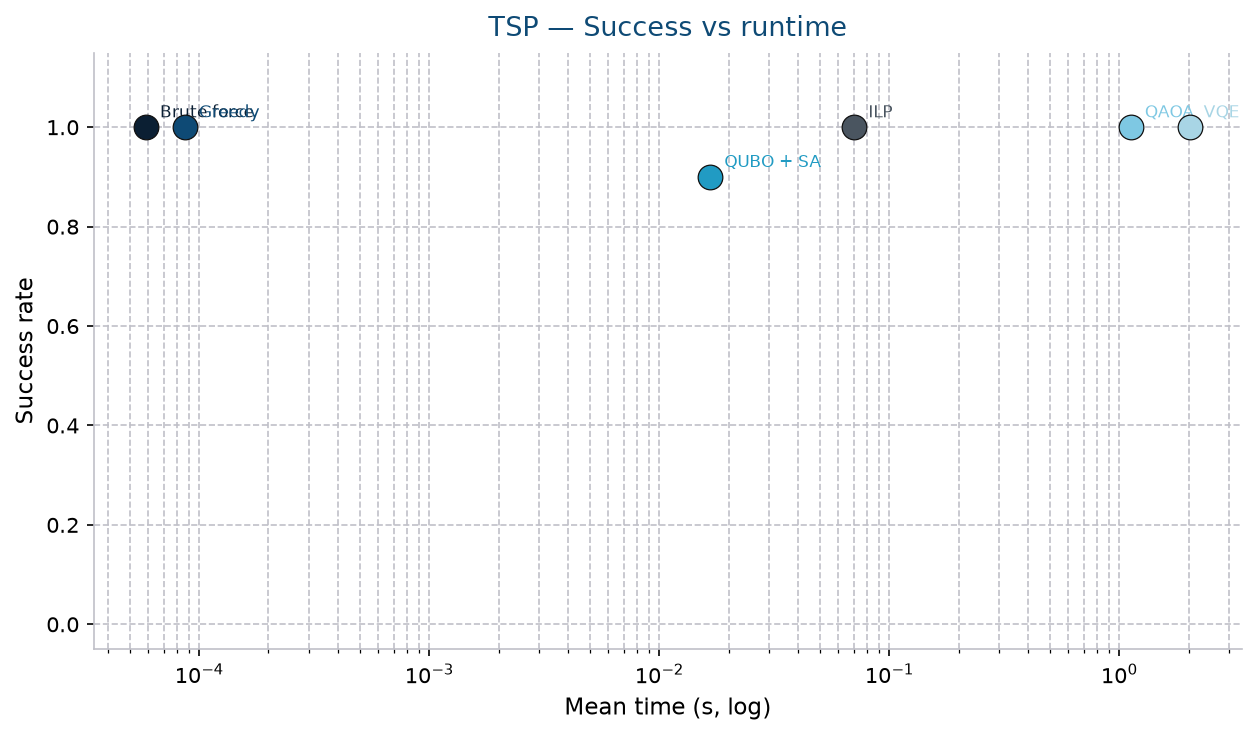
\includegraphics[width=0.72\textwidth]{tsp_success_vs_runtime.png}
\caption{TSP: success rate frente al tiempo. El SA es el único que no satura el éxito; ILP, QAOA y VQE comparten la escala del segundo.}
\label{fig:tsp_success}
\end{figure}

\subsubsection{Fuerza bruta}

Enumera las rutas y devuelve $C^\star$ en menos de un milisegundo ($6$ evaluaciones de la función de coste). La Figura~\ref{fig:tsp_bf} es una ruta óptima. Con 5 nodos el espacio de tours es el método de referencia, no un baseline débil: cualquier otro solver se juzga contra una enumeración que ya es barata.

\begin{figure}[!htbp]
\centering
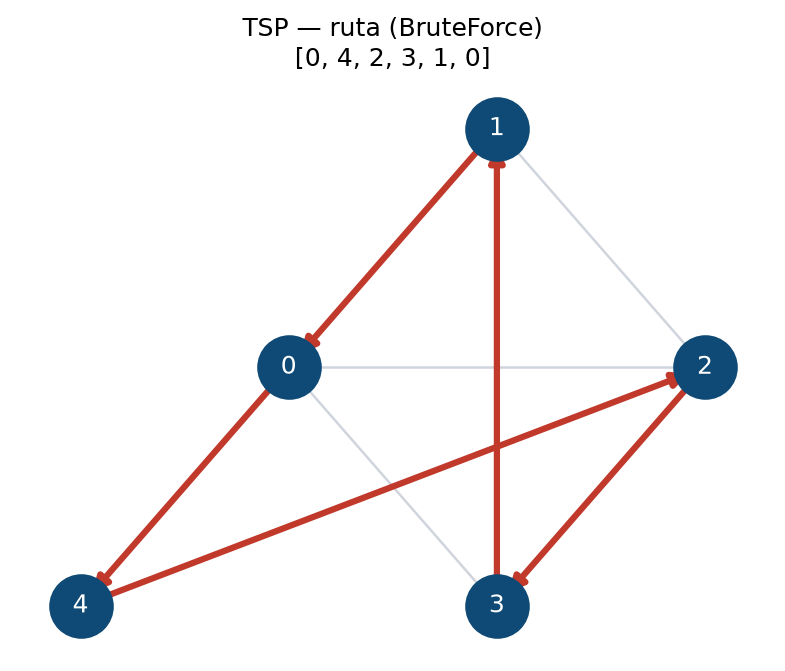
\includegraphics[width=0.62\textwidth]{bruteforce_tsp_route.png}
\caption{Ruta óptima del TSP por enumeración. Coste $16$.}
\label{fig:tsp_bf}
\end{figure}

\subsubsection{Greedy}

La heurística de vecino más cercano también cierra en $16$ (Figura~\ref{fig:tsp_greedy}), en $0.5\,\mathrm{ms}$. En este grafo el óptimo local coincide con el global. No es una propiedad del algoritmo: en MDS, con la misma heurística, el conjunto se pasa de tamaño. Aquí el grafo es pequeño y las distancias no castigan el primer paso miope.

\begin{figure}[!htbp]
\centering
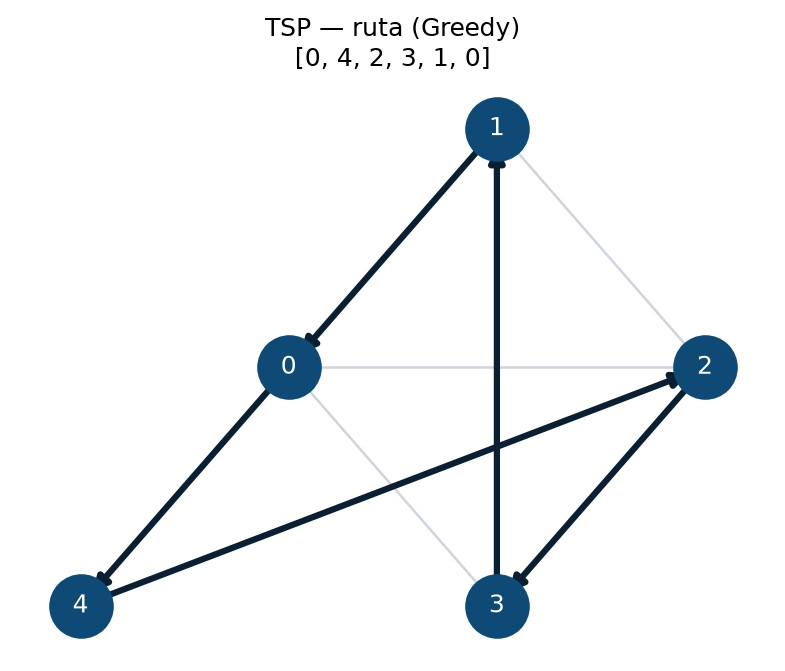
\includegraphics[width=0.62\textwidth]{greedy_tsp_route.png}
\caption{Ruta del greedy en el TSP. El coste coincide con el óptimo.}
\label{fig:tsp_greedy}
\end{figure}

\subsubsection{ILP}

La formulación lineal con CBC devuelve el óptimo y tarda $1.28\,\mathrm{s}$. Ese tiempo es de arranque del solver, no de una búsqueda larga: la fuerza bruta, sobre el mismo espacio, termina en menos de un milisegundo. La Figura~\ref{fig:tsp_ilp} certifica la ruta. El ILP importa como método exacto general; en esta instancia no es el exacto más rápido.

\begin{figure}[!htbp]
\centering
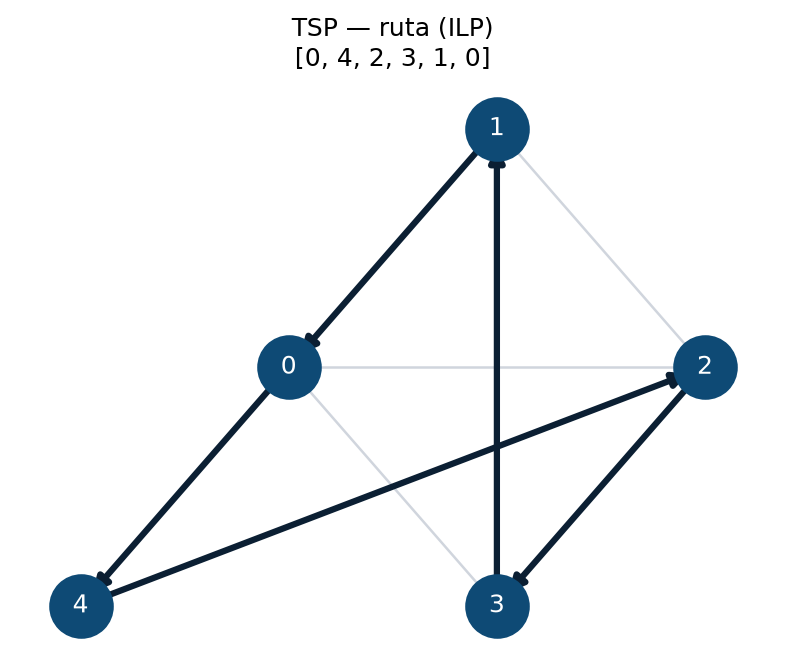
\includegraphics[width=0.62\textwidth]{ilp_tsp_route.png}
\caption{Ruta del ILP en el TSP. Óptimo de coste $16$, con el mayor tiempo clásico de la tabla.}
\label{fig:tsp_ilp}
\end{figure}

\subsubsection{QUBO + simulated annealing}

El annealing sobre el QUBO acierta el óptimo en el $90\%$ de las semillas. La media de coste sube a $16.3$ (gap relativo $0.019$) con unas $5000$ evaluaciones y $0.017\,\mathrm{s}$. La Figura~\ref{fig:tsp_sa} muestra una semilla óptima, la ruta $[0,4,2,3,1,0]$. La técnica es clásica y opera en la misma energía que QAOA y VQE: cuando la penalización del QUBO está bien puesta, el recocido encuentra el tour; una semilla de cada diez cae en un coste vecino. Es el único solver del TSP que no tiene éxito $1$, y sigue siendo dos órdenes más rápido que el circuito simulado.

\begin{figure}[!htbp]
\centering
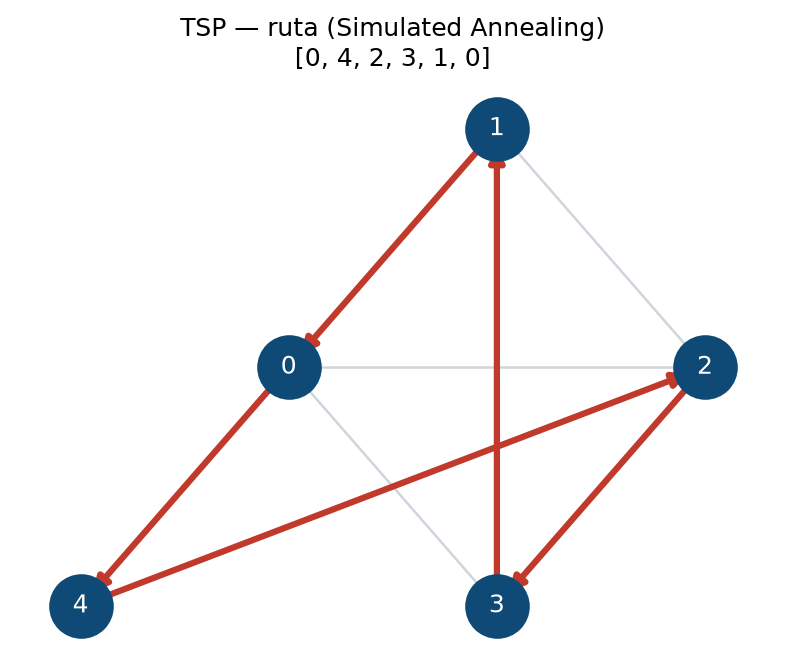
\includegraphics[width=0.62\textwidth]{sa_tsp_route.png}
\caption{Una ruta óptima del simulated annealing, $[0,4,2,3,1,0]$. El success rate sobre semillas es $0.90$.}
\label{fig:tsp_sa}
\end{figure}

\subsubsection{QAOA}

Capas $U_C U_B$ sobre el mismo QUBO, en simulación de estado, alcanzan coste $16$ en las ejecuciones reportadas (éxito $1$, unas $356$ evaluaciones, $1.06\,\mathrm{s}$). La Figura~\ref{fig:tsp_qaoa} es el tour devuelto. QAOA reproduce el óptimo que la enumeración ya tiene, en un tiempo del orden del ILP y muy por encima del annealing. Con 5 nodos el circuito no explora un espacio que el clásico no enumere; mide si el ansatz variacional concentra probabilidad en la ruta óptima \citep{farhi2014}. Aquí sí. El coste es el de simular esas capas.

\begin{figure}[!htbp]
\centering
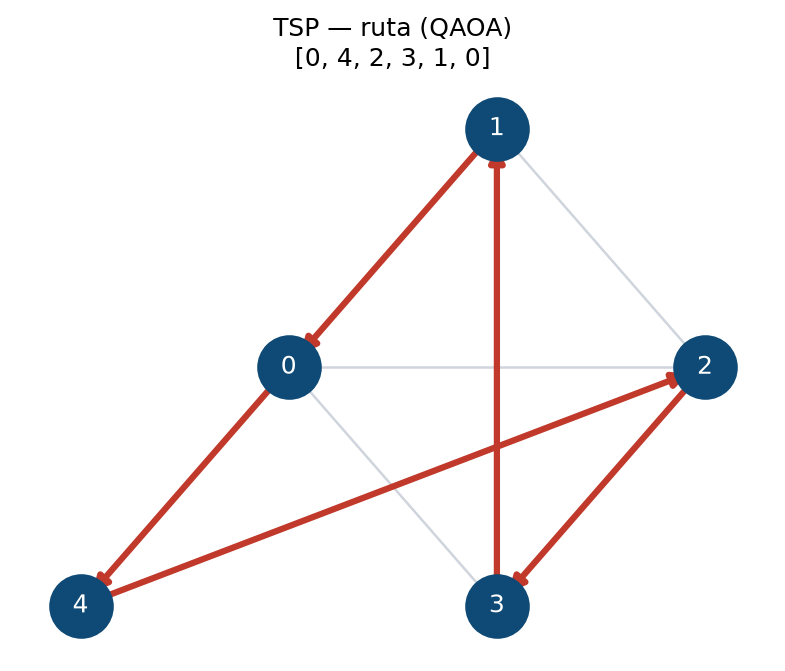
\includegraphics[width=0.62\textwidth]{qaoa_tsp_route.png}
\caption{Ruta devuelta por QAOA en el TSP. Coste óptimo, en torno a un segundo de simulación.}
\label{fig:tsp_qaoa}
\end{figure}

\subsubsection{VQE}

El ansatz variacional minimiza la energía del Ising equivalente y también devuelve coste $16$ (Figura~\ref{fig:tsp_vqe}), con unas $720$ evaluaciones y $1.91\,\mathrm{s}$, el mayor tiempo del problema. La diferencia con QAOA no está en la calidad, que satura, sino en el número de evaluaciones del Hamiltoniano y en que el ansatz no está estructurado como la alternancia coste--mezclador. En una instancia enumerable, VQE es una comprobación de que el óptimo es un mínimo del QUBO, no un algoritmo más corto que la fuerza bruta \citep{peruzzo2014}.

\begin{figure}[!htbp]
\centering
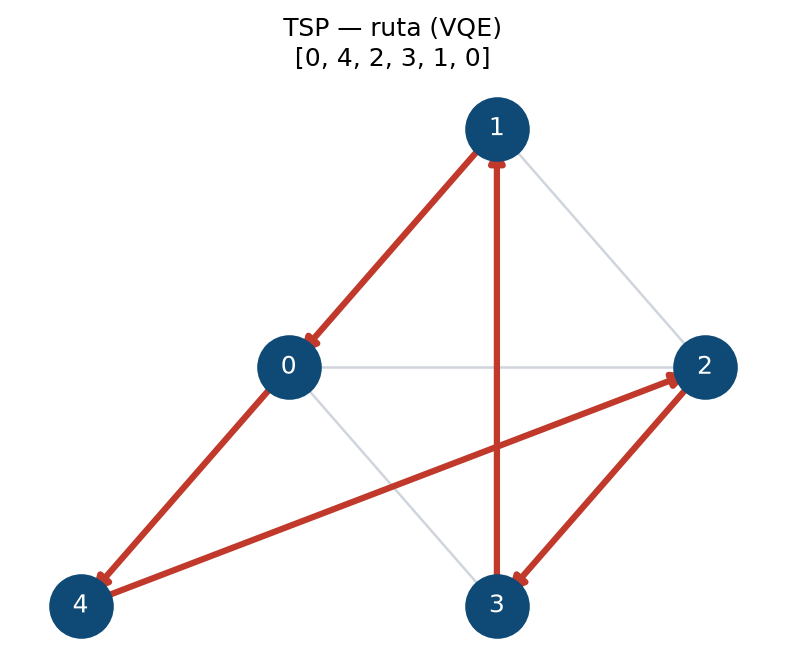
\includegraphics[width=0.62\textwidth]{vqe_tsp_route.png}
\caption{Ruta devuelta por VQE en el TSP. Mismo coste óptimo, más evaluaciones de energía que QAOA.}
\label{fig:tsp_vqe}
\end{figure}

\subsection{Minimum dominating set}

Grafo de 6 vértices y 6 aristas. El óptimo es un conjunto de tamaño $2$. Es la instancia que separa heurística, annealing y circuito (Tabla~\ref{tab:res_mds}).

\begin{table}[!htbp]
\centering
\small
\resizebox{\textwidth}{!}{%
\begin{tabular}{lrrrrrr}
\toprule
\textbf{Solver} & \textbf{Éxito} & $C$ medio & $C$ mejor & \textbf{Gap} & \textbf{Gap rel.} & $t$ (s) \\
\midrule
Fuerza bruta & 1.00 & 2.00 & 2 & 0.00 & 0.000 & 0.0002 \\
Greedy & 0.00 & 3.00 & 3 & 1.00 & 0.500 & $<0.001$ \\
ILP & 1.00 & 2.00 & 2 & 0.00 & 0.000 & 0.666 \\
QUBO + SA & 1.00 & 2.00 & 2 & 0.00 & 0.000 & 0.008 \\
QAOA & 0.875 & 2.25 & 2 & 0.25 & 0.125 & 12.232 \\
VQE & 1.00 & 2.00 & 2 & 0.00 & 0.000 & 1.561 \\
\bottomrule
\end{tabular}}
\caption{MDS. $C^\star=2$. QAOA promedia semillas; el mejor coste de esas semillas sigue siendo $2$.}
\label{tab:res_mds}
\end{table}

\begin{figure}[!htbp]
\centering
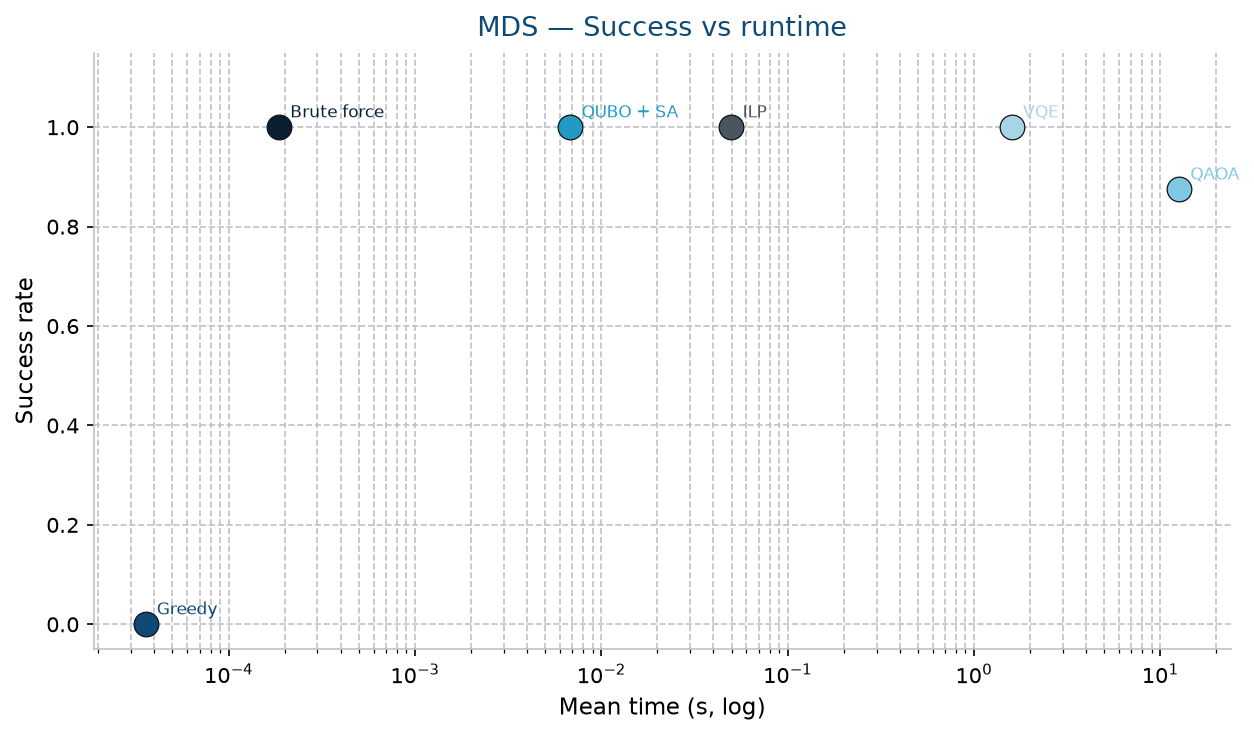
\includegraphics[width=0.72\textwidth]{mds_success_vs_runtime.png}
\caption{MDS: success rate frente al tiempo. Greedy no acierta; QAOA acierta en una fracción de las semillas y es el más lento.}
\label{fig:mds_success}
\end{figure}

\subsubsection{Fuerza bruta}

Enumera subconjuntos y fija $C^\star=2$ en $0.2\,\mathrm{ms}$. La Figura~\ref{fig:mds_bf} es un conjunto dominante mínimo. Con 6 vértices, $2^6=64$ máscaras: el óptimo de referencia sale antes de que un solver iterativo arranque.

\begin{figure}[!htbp]
\centering
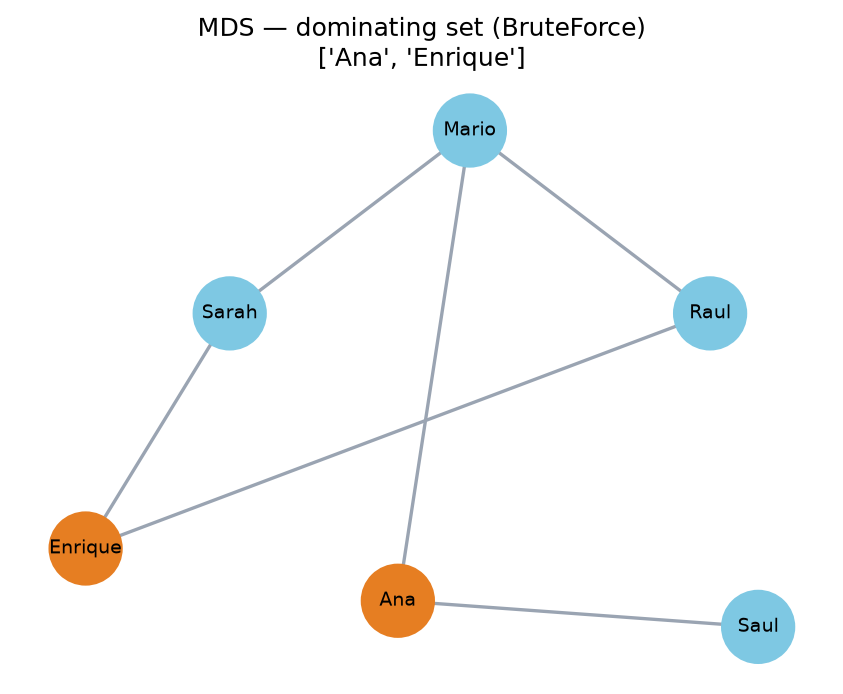
\includegraphics[width=0.62\textwidth]{bruteforce_mds_dominating_set.png}
\caption{Conjunto dominante mínimo por enumeración. Tamaño $2$.}
\label{fig:mds_bf}
\end{figure}

\subsubsection{Greedy}

Elige Mario, Sarah y Ana (Figura~\ref{fig:mds_greedy}): tamaño $3$, gap $1$, gap relativo $0.5$, éxito $0$. La heurística cubre por grado local y no deshace la primera elección. Enrique y Ana solos dominan el grafo; el greedy no llega a ese par porque ya ha gastado un vértice. Es el único fallo sistemático de la familia clásica y no se arregla con más tiempo: la regla es determinista. En grafos de cobertura, un voraz sin backtracking no es un baseline de calidad, es una cota rápida que aquí queda corta.

\begin{figure}[!htbp]
\centering
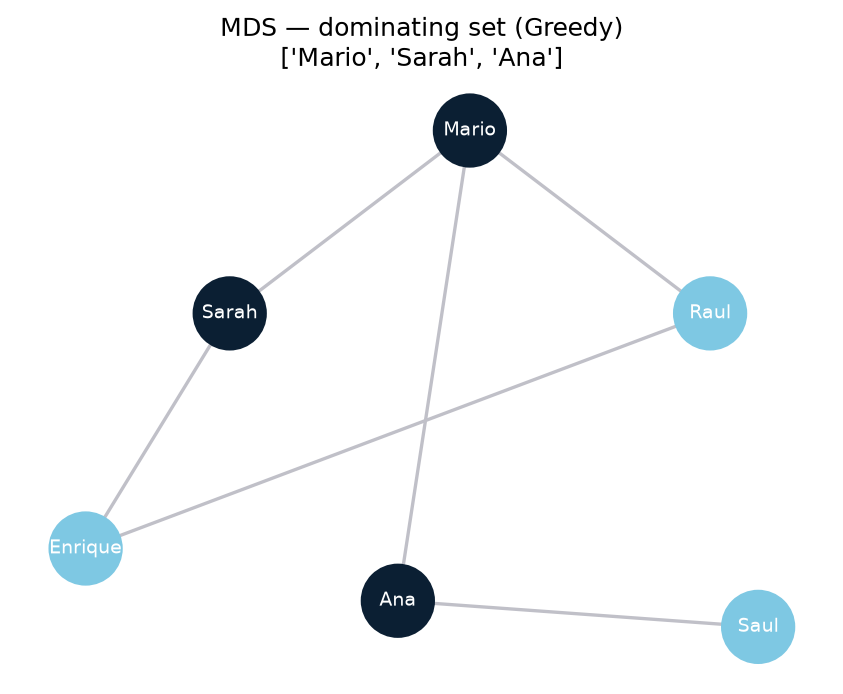
\includegraphics[width=0.62\textwidth]{greedy_mds_dominating_set.png}
\caption{Conjunto del greedy: Mario, Sarah y Ana. Tamaño $3$, uno por encima del óptimo.}
\label{fig:mds_greedy}
\end{figure}

\subsubsection{ILP}

La cobertura lineal con CBC devuelve un conjunto de tamaño $2$ en $0.67\,\mathrm{s}$ (Figura~\ref{fig:mds_ilp}). El modelo es exacto: cada vértice queda dominado y la objetivo minimiza la suma de binarias. El tiempo, como en el TSP, incluye el arranque de CBC. Frente al greedy, el ILP paga décimas de segundo y cierra el gap. Frente a la enumeración, es más lento y igual de correcto.

\begin{figure}[!htbp]
\centering
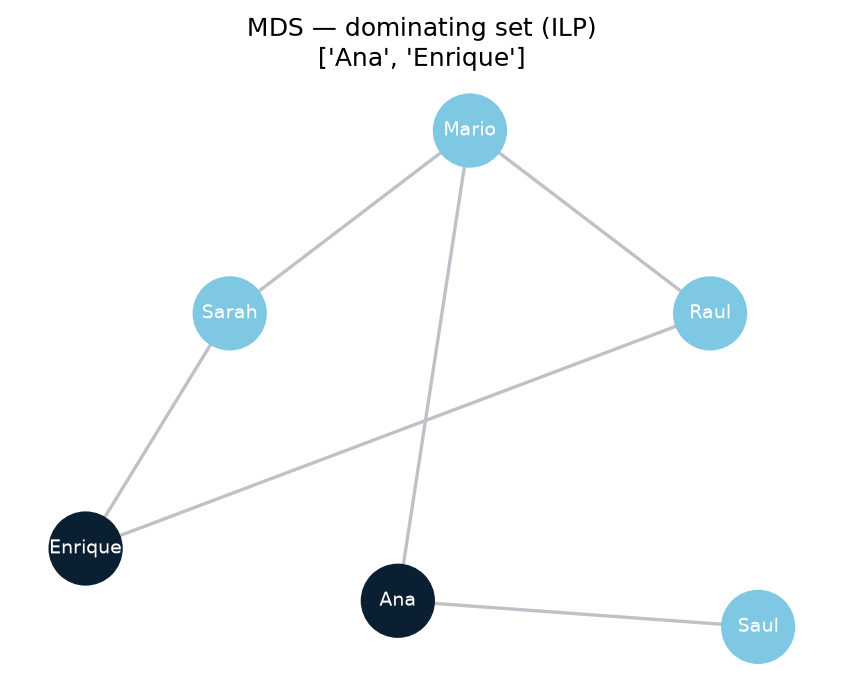
\includegraphics[width=0.62\textwidth]{ilp_mds_dominating_set.png}
\caption{Conjunto dominante del ILP. Tamaño óptimo $2$.}
\label{fig:mds_ilp}
\end{figure}

\subsubsection{QUBO + simulated annealing}

El annealing sobre el QUBO de cobertura acierta tamaño $2$ en todas las semillas reportadas, con unas $4000$ evaluaciones y $0.008\,\mathrm{s}$ (Figura~\ref{fig:mds_sa}). La misma energía que luego ven QAOA y VQE ya es minimizable por recocido clásico. En esta instancia la formulación QUBO no deforma el óptimo: si la penalización de no-dominancia está bien escalada, el SA cae en $C^\star$ \citep{lucas2014}. El contraste con el TSP, donde una semilla fallaba, es de paisaje, no de método.

\begin{figure}[!htbp]
\centering
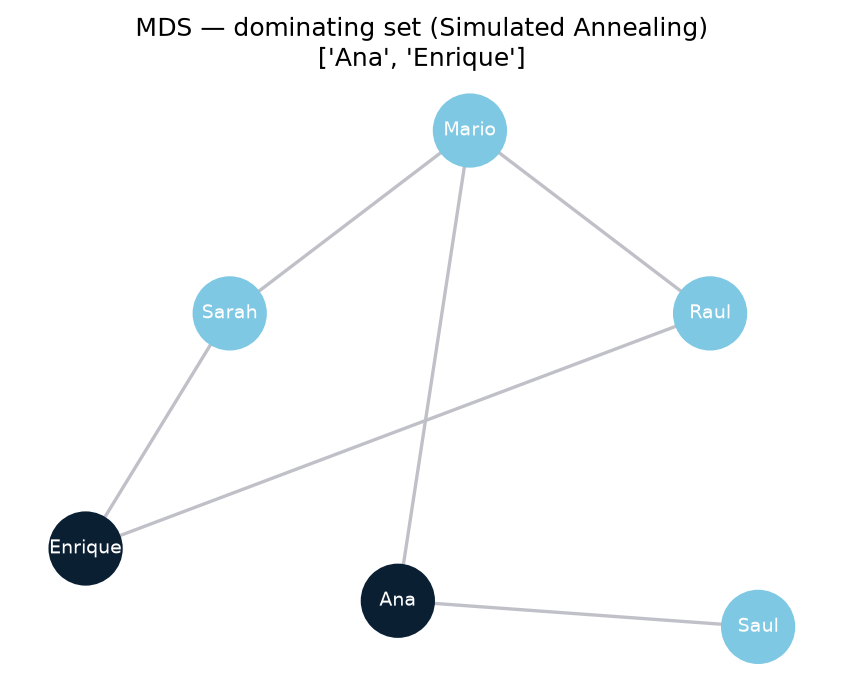
\includegraphics[width=0.62\textwidth]{sa_mds_dominating_set.png}
\caption{Conjunto devuelto por simulated annealing. Tamaño $2$ en las semillas reportadas.}
\label{fig:mds_sa}
\end{figure}

\subsubsection{QAOA}

Es el resultado cuántico-inspirado que no satura. Éxito $0.875$, coste medio $2.25$, gap $0.25$, unas $4000$ evaluaciones y $12.2\,\mathrm{s}$, el máximo de todo el corpus de optimización. La Figura~\ref{fig:mds_qaoa} es una semilla óptima: Ana y Enrique, tamaño $2$. Otras semillas salen con un vértice de más, y por eso la media no es $2$. El ansatz $U_C U_B$ ve el mismo QUBO que el SA, que sí acierta siempre y en milisegundos. La discusión es de optimización variacional, no de formulación: con pocas capas y en simulación, la distribución de medida no concentra toda la masa en el bitstring óptimo \citep{farhi2014, lubinski2024}. Subir capas alargaría aún más la simulación.

\begin{figure}[!htbp]
\centering
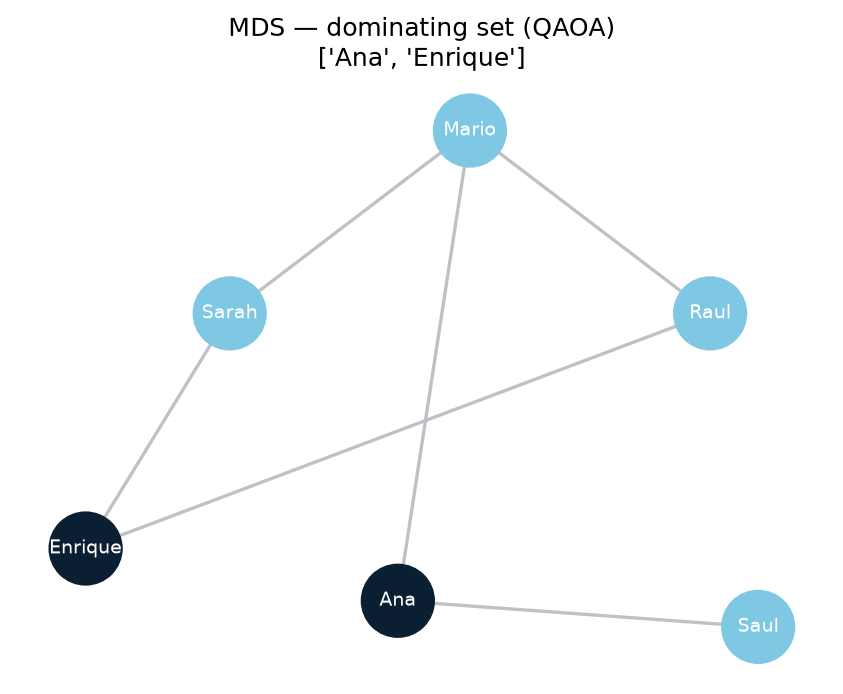
\includegraphics[width=0.62\textwidth]{qaoa_mds_dominating_set.png}
\caption{Una ejecución óptima de QAOA: Ana y Enrique. El success rate sobre semillas es $0.875$.}
\label{fig:mds_qaoa}
\end{figure}

\subsubsection{VQE}

Alcanza tamaño $2$ en las semillas reportadas (Figura~\ref{fig:mds_vqe}), con unas $600$ evaluaciones y $1.56\,\mathrm{s}$. El mismo problema en el que QAOA oscila, el VQE lo cierra. El ansatz y el número de evaluaciones no son los de QAOA: aquí bastan menos llamadas al Hamiltoniano para clavar el mínimo que el SA ya encontraba. Sigue siendo dos órdenes más lento que el annealing y tres que la enumeración. La técnica confirma el mínimo del Ising; no acorta la búsqueda en un grafo de 6 vértices \citep{peruzzo2014}.

\begin{figure}[!htbp]
\centering
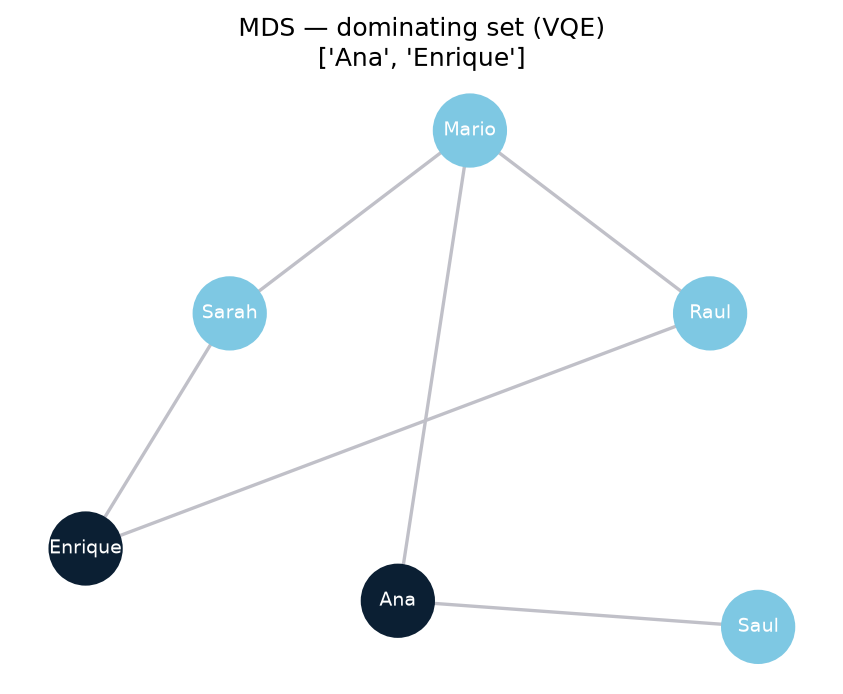
\includegraphics[width=0.62\textwidth]{vqe_mds_dominating_set.png}
\caption{Conjunto devuelto por VQE. Tamaño óptimo, por debajo del tiempo de QAOA y por encima del SA.}
\label{fig:mds_vqe}
\end{figure}

\subsection{MaxCut}

Instancia HamLib de 6 vértices y 12 aristas, corte óptimo $8$. Los seis solvers lo alcanzan (Tabla~\ref{tab:res_maxcut}). La figura de cada implementación es la partición que realiza ese corte.

\begin{table}[!htbp]
\centering
\small
\resizebox{\textwidth}{!}{%
\begin{tabular}{lrrrrrr}
\toprule
\textbf{Solver} & \textbf{Éxito} & $C$ medio & $C$ mejor & \textbf{Gap} & \textbf{Gap rel.} & $t$ (s) \\
\midrule
Fuerza bruta & 1.00 & 8 & 8 & 0 & 0 & $7\cdot 10^{-5}$ \\
Greedy & 1.00 & 8 & 8 & 0 & 0 & $4\cdot 10^{-5}$ \\
ILP & 1.00 & 8 & 8 & 0 & 0 & 0.011 \\
QUBO + SA & 1.00 & 8 & 8 & 0 & 0 & 0.004 \\
QAOA & 1.00 & 8 & 8 & 0 & 0 & 1.247 \\
VQE & 1.00 & 8 & 8 & 0 & 0 & 1.799 \\
\bottomrule
\end{tabular}}
\caption{MaxCut HamLib. $C^\star=8$. Todos los solvers reportados alcanzan el corte óptimo.}
\label{tab:res_maxcut}
\end{table}

\begin{figure}[!htbp]
\centering
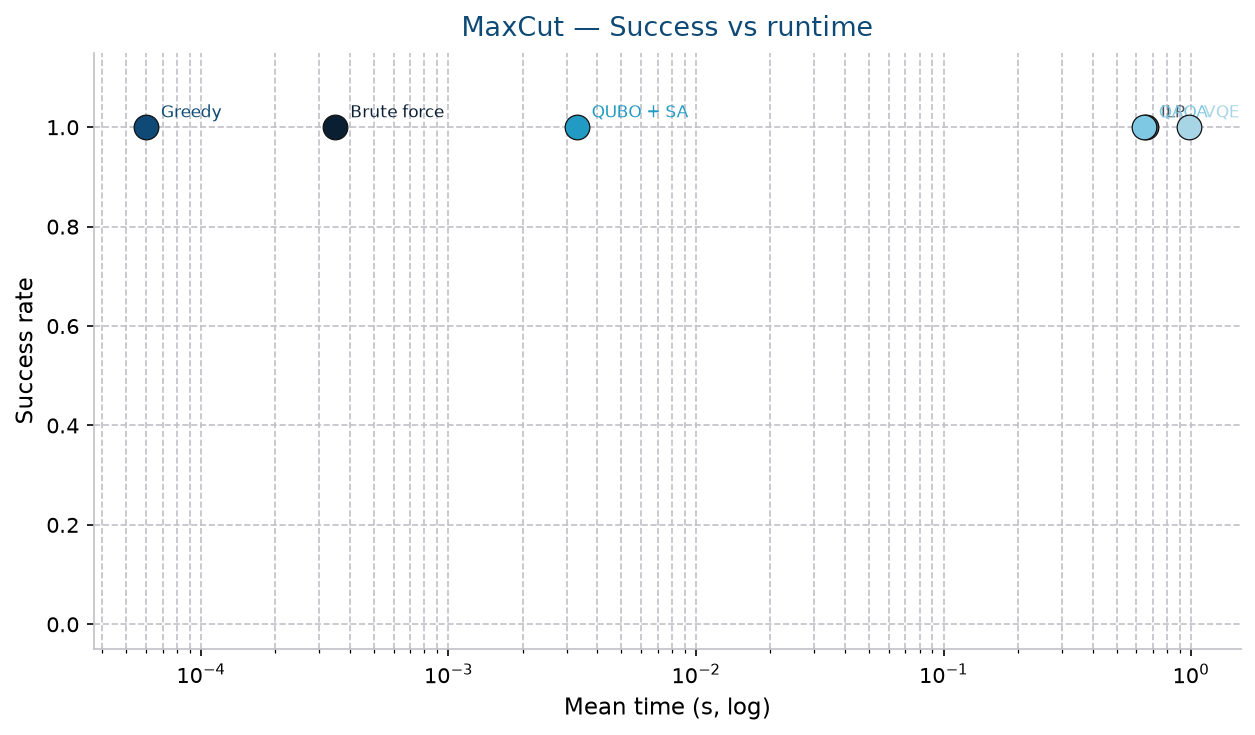
\includegraphics[width=0.72\textwidth]{maxcut_success_vs_runtime.png}
\caption{MaxCut: éxito $1$ para todos los solvers. El eje de tiempo separa enumeración, greedy y SA del ILP y, más allá, de QAOA y VQE.}
\label{fig:maxcut_success}
\end{figure}

\subsubsection{Fuerza bruta}

Evalúa las $2^6$ biparticiones y devuelve corte $8$ en decenas de microsegundos (Figura~\ref{fig:maxcut_bf}). En MaxCut el espacio es el de asignar un bit por vértice, exactamente el espacio de un circuito de 6 qubits, y la enumeración lo recorre entero. El óptimo de referencia queda fijado antes de hablar de ansatz.

\begin{figure}[!htbp]
\centering
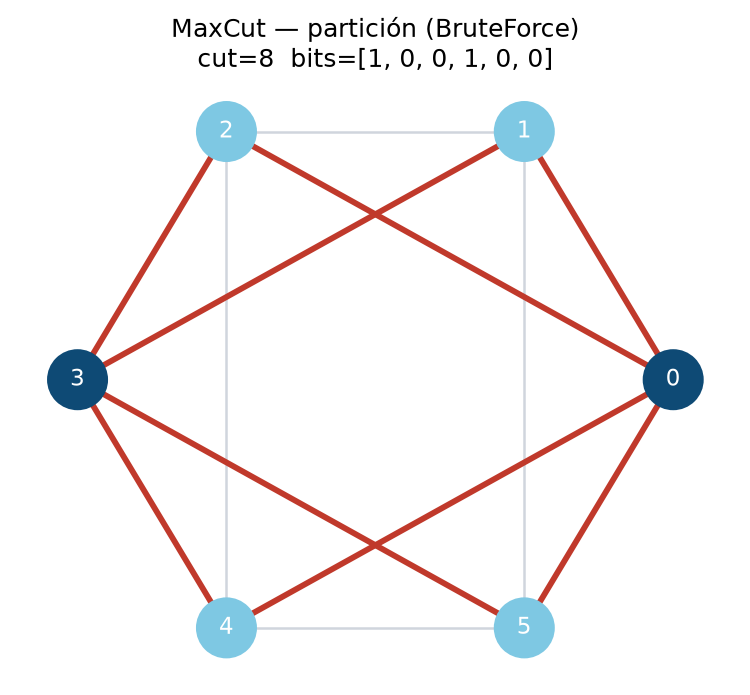
\includegraphics[width=0.62\textwidth]{bruteforce_maxcut_cut.png}
\caption{Corte óptimo de MaxCut por enumeración. Valor $8$.}
\label{fig:maxcut_bf}
\end{figure}

\subsubsection{Greedy}

También corta $8$ (Figura~\ref{fig:maxcut_greedy}), aún más rápido. A diferencia del MDS, en esta instancia el crecimiento local de la partición no se queda corto. El grafo es denso (12 aristas sobre 6 vértices) y varios cortes alcanzan el óptimo, así que una heurística miope tiene donde acertar. No se generaliza al MDS, donde el mismo tipo de regla falló.

\begin{figure}[!htbp]
\centering
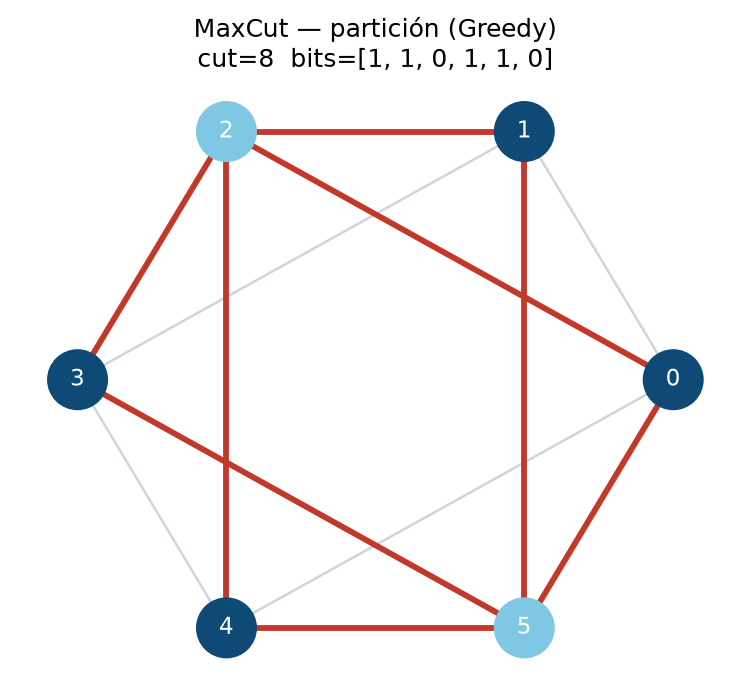
\includegraphics[width=0.62\textwidth]{greedy_maxcut_cut.png}
\caption{Corte del greedy en MaxCut. Valor óptimo $8$.}
\label{fig:maxcut_greedy}
\end{figure}

\subsubsection{ILP}

CBC devuelve corte $8$ en $0.011\,\mathrm{s}$ (Figura~\ref{fig:maxcut_ilp}). El modelo lineal de MaxCut es compacto en 6 vértices y el arranque del solver pesa menos que en el TSP. Sigue siendo exacto y más lento que enumerar 64 asignaciones. Su papel en el protocolo es el método exacto de formulación nativa, al lado del QUBO que usan SA, QAOA y VQE.

\begin{figure}[!htbp]
\centering
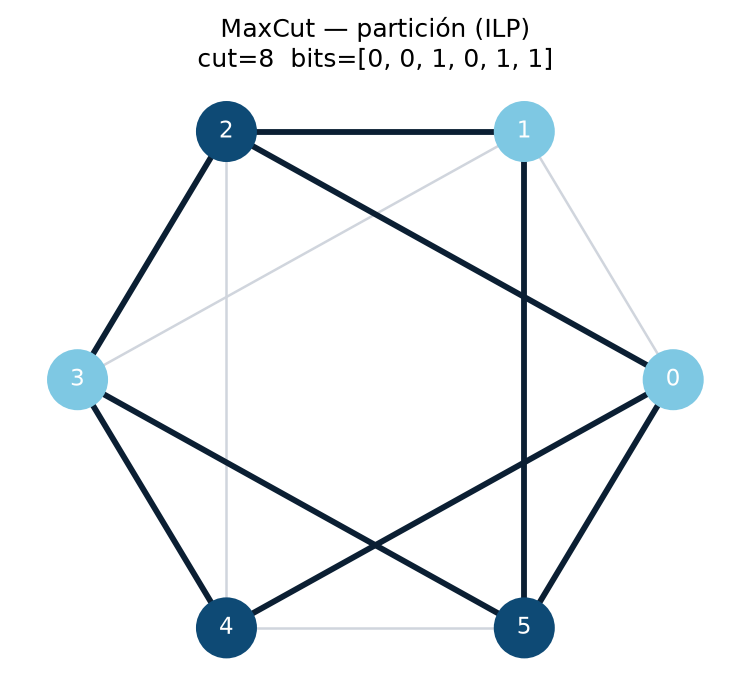
\includegraphics[width=0.62\textwidth]{ilp_maxcut_cut.png}
\caption{Corte del ILP en MaxCut. Valor $8$.}
\label{fig:maxcut_ilp}
\end{figure}

\subsubsection{QUBO + simulated annealing}

Corte $8$ en todas las semillas, unas $4000$ evaluaciones, $0.004\,\mathrm{s}$ (Figura~\ref{fig:maxcut_sa}). El QUBO de MaxCut no lleva restricciones de igualdad duras: la objetivo es el corte, y el paisaje que ve el SA es el mismo que el Hamiltoniano de coste de QAOA. Aquí el recocido clásico encuentra el mínimo que el circuito también encuentra, tres órdenes de magnitud antes.

\begin{figure}[!htbp]
\centering
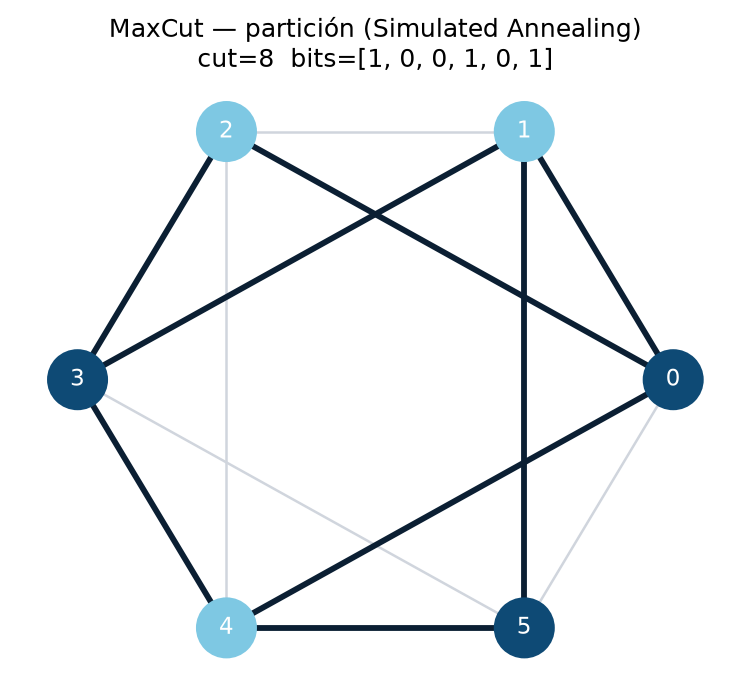
\includegraphics[width=0.62\textwidth]{sa_maxcut_cut.png}
\caption{Corte del simulated annealing en MaxCut. Valor óptimo en las semillas reportadas.}
\label{fig:maxcut_sa}
\end{figure}

\subsubsection{QAOA}

Corte $8$, éxito $1$, unas $40$ evaluaciones, $1.25\,\mathrm{s}$ (Figura~\ref{fig:maxcut_qaoa}). Pocas evaluaciones bastan porque el problema es el ejemplo estándar del ansatz: $U_C$ es el Hamiltoniano del corte y $U_B$ mezcla las biparticiones \citep{farhi2014, pennylaneQaoaMaxcut}. La calidad empata con la enumeración. El tiempo es el de simular el estado de 6 qubits, no el de probar 64 cortes. En la comparación cuantitativa, QAOA demuestra que el circuito codifica el problema; no que lo resuelva antes que recorrerlo.

\begin{figure}[!htbp]
\centering
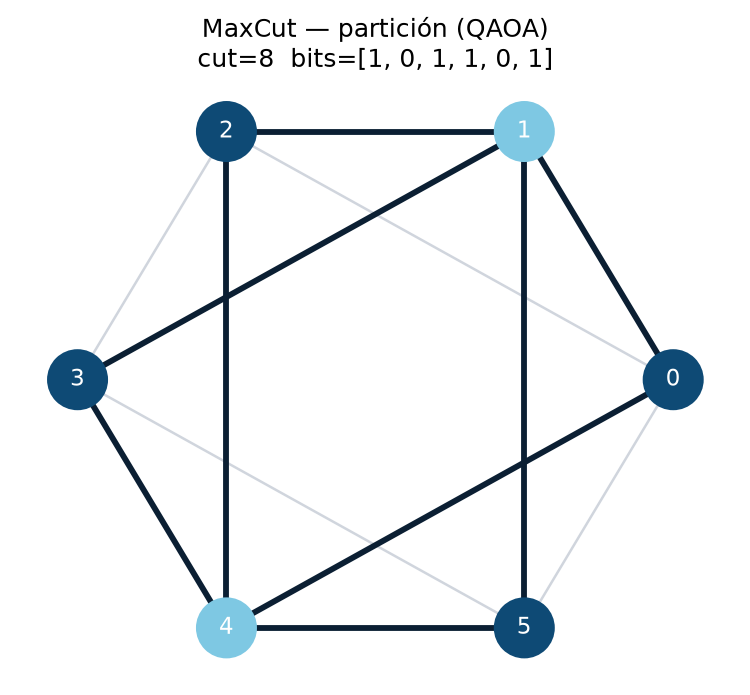
\includegraphics[width=0.62\textwidth]{qaoa_maxcut_cut.png}
\caption{Corte devuelto por QAOA. Valor óptimo $8$, en torno a $1.2\,\mathrm{s}$ de simulación.}
\label{fig:maxcut_qaoa}
\end{figure}

\subsubsection{VQE}

Corte $8$, unas $240$ evaluaciones, $1.80\,\mathrm{s}$ (Figura~\ref{fig:maxcut_vqe}). Más llamadas al Hamiltoniano que QAOA para el mismo corte: el ansatz genérico no trae la alternancia coste--mezclador que ya es el algoritmo de MaxCut. La calidad no distingue a los dos. El número de evaluaciones sí, y ambos quedan lejos de los $7\cdot 10^{-5}\,\mathrm{s}$ de la enumeración \citep{peruzzo2014, lubinski2024}.

\begin{figure}[!htbp]
\centering
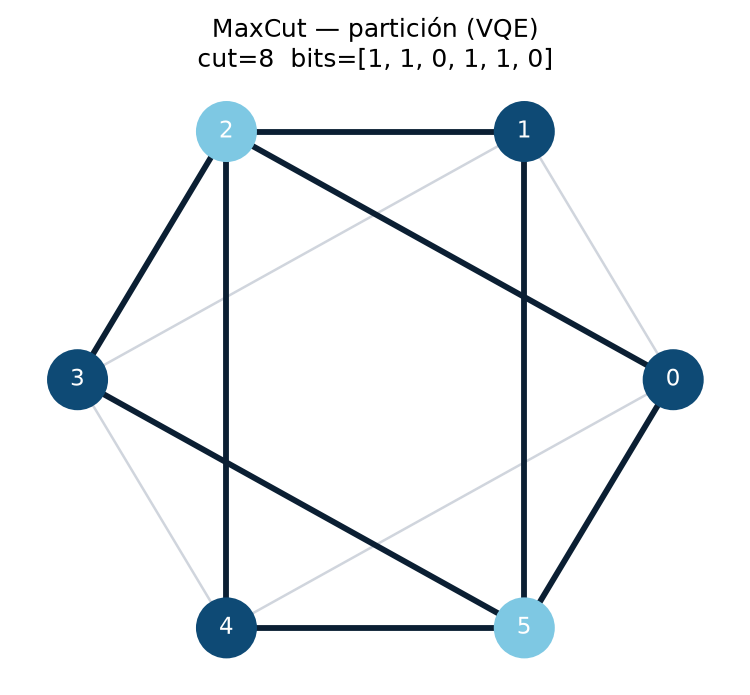
\includegraphics[width=0.62\textwidth]{vqe_maxcut_cut.png}
\caption{Corte devuelto por VQE. Mismo óptimo que QAOA, con más evaluaciones de energía.}
\label{fig:maxcut_vqe}
\end{figure}

\subsection{Lectura de la familia}

En las tres instancias el óptimo es alcanzable por enumeración en menos de un milisegundo. El ILP también es exacto; su wall-clock mide el arranque de CBC, que en el TSP llega al segundo y en MaxCut baja a centésimas. El greedy solo falla en MDS, donde la elección local produce un conjunto de tamaño $3$ y el óptimo es $2$. El SA sobre QUBO empata con el óptimo en MDS y MaxCut y se deja una semilla de cada diez en el TSP, siempre en centésimas de segundo. QAOA y VQE, en simulación, recuperan $C^\star$ salvo QAOA en MDS (éxito $0.875$, $12.2\,\mathrm{s}$). Cuando aciertan, el circuito está bien planteado sobre el QUBO; el tiempo es el de evaluar el ansatz, no una búsqueda más corta que $2^n$ en $n\le 6$ \citep{farhi2014, lubinski2024}. La lectura conjunta de calidad y latencia, en este régimen, es que el óptimo ya está en los métodos exactos clásicos y en el annealing, y que el circuito lo reproduce con un coste de simulación mayor.

% !TEX root = ../main.tex
\chapter{Conclusiones}\label{cap:conclusiones}

El trabajo partió de una pregunta: si los algoritmos cuánticos de la era NISQ ofrecen una ventaja medible frente a los clásicos en problemas de ciencia de datos. Para responderla se compararon seis modelos de clasificación sobre Iris, Bars and Stripes e Ising y seis solvers de optimización sobre TSP, MDS y MaxCut, con un protocolo común y la representación como eje de lectura. Las conclusiones siguen de los resultados del Capítulo~\ref{cap:evaluacion}.

\section{Conclusiones}

\begin{enumerate}
\item \textbf{En clasificación no se observa ventaja cuántica.} El SVM con kernel RBF obtiene el mejor F1 o empata con el mejor en los tres datasets (0.967 en Iris, 0.870 en Bars and Stripes, 0.985 en Ising) y es el más rápido de entrenar. Ningún modelo cuántico lo supera. La media cuántica de accuracy queda 0.083 y 0.101 por debajo de la clásica en Iris y Bars and Stripes, y la iguala en Ising.

\item \textbf{El QSVM con mapa ZZ solo alcanza al clásico en el dataset más fácil.} Empata con el SVM en Ising (F1 0.985), donde los seis modelos alcanzan al menos 0.95 de accuracy, y cae a 0.730 en Iris y 0.758 en Bars and Stripes, con el mayor gap de generalización del corpus en Iris (0.233). El experimento no aísla la causa del empate en Ising: el mapa actúa sobre componentes principales de las amplitudes, no sobre los espines de la cadena.

\item \textbf{Los modelos variacionales se acercan al clásico sin superarlo.} La QNN híbrida es el modelo cuántico más regular (F1 0.933, 0.815 y 0.937, con gap de generalización $\le 0.022$). El VQC iguala a los árboles en Iris (0.950), queda el último en Bars and Stripes (0.688) y es el más caro de entrenar en los tres datasets.

\item \textbf{En optimización, QAOA y VQE reproducen el óptimo, pero no mejoran a los métodos clásicos.} Los métodos exactos alcanzan $C^\star$ en las tres instancias, la enumeración en menos de un milisegundo. El annealing simulado lo hace sobre la misma formulación QUBO en milisegundos (éxito 0.9 en TSP y 1 en MDS y MaxCut). QAOA y VQE llegan al óptimo en TSP y MaxCut, y VQE también en MDS, con entre 0.6 y 2~s de simulación. En MDS una de las ocho semillas de QAOA devuelve una solución infactible (éxito 0.875, 12.6~s): termina con mayor energía esperada y probabilidad nula de medir el óptimo, mientras que el annealing sobre el mismo QUBO acierta siempre. Como en TSP y MDS ambos leen el mejor de miles de bitstrings, su éxito en esos casos no prueba que el circuito concentre probabilidad en el óptimo.

\item \textbf{El régimen estudiado mide proximidad al clásico, no ventaja.} Con 4 qubits en clasificación, como mucho 6 en optimización y simulación de estado exacta, los resultados no permiten afirmar ni descartar una ventaja a escala \citep{preskill2018, thanasilp2022}. Sí permiten afirmar que, en este rango, ningún modelo o solver cuántico supera al mejor clásico, y que la paridad de calidad, cuando aparece, va acompañada de un coste temporal mayor.
\end{enumerate}

% !TEX root = ../main.tex
\chapter{Líneas futuras de investigación}
\label{cap:futuro}

La Tabla~\ref{tab:futuro} recoge las líneas que extienden el estudio. Todas mantienen el criterio de comparación: el modelo cuántico frente al mejor clásico, con el mismo protocolo.

\begin{table}[!htbp]
\centering
\footnotesize
\renewcommand{\arraystretch}{1.1}
\begin{tabularx}{\textwidth}{@{}>{\raggedright\arraybackslash}p{0.22\textwidth}>{\raggedright\arraybackslash}X@{}}
\toprule
\textbf{Línea} & \textbf{Qué se propone} \\
\midrule
Más qubits en hardware cuántico & Ejecutar los casos con más qubits en hardware real, por shots y con mitigación de errores, con instancias mayores de HamLib \citep{sawaya2024hamlib, pennylaneHamlibTsp}, kernels estimados por medidas aleatorizadas \citep{haug2023} y compilación estructurada \citep{rovara2026}. \\
\addlinespace
Mapeos de representación & Comparar otros feature maps y codificaciones: basis encoding, re-uploading \citep{perezSalinas2020}, embeddings entrenables \citep{lloyd2020} y elección del circuito según la complejidad del dato \citep{dePaulaNeto2025}. \\
\addlinespace
Más familias de casos de uso & Extender el protocolo a clusterización \citep{aimeur2007, sentis2019, kerenidis2019qmeans}, series de tiempo, regresión \citep{friedman1991, kulkarniQlr} y simulación. \\
\addlinespace
Reducción de dimensionalidad & Sustituir la PCA por otros métodos, clásicos y cuánticos, como qPCA o autoencoders cuánticos \citep{lloyd2014, romero2017}, con la salvedad de \citet{tang2021}. \\
\addlinespace
Instancias diferentes a QUBO & Problemas cuya formulación natural no es cuadrática, como Max-$k$-SAT, y otras familias de Hamiltonianos de HamLib \citep{sawaya2024hamlib}. \\
\addlinespace
Diferentes conjuntos de datos & Repetir la comparación sobre otros datasets, reales y sintéticos, como los del benchmark de \citet{bowles2024}. \\
\bottomrule
\end{tabularx}
\caption{Líneas futuras de investigación.}
\label{tab:futuro}
\end{table}

% !TEX root = ../main.tex
\begin{thebibliography}{99}

	\bibitem[A\"imeur et~al.(2007)]{aimeur2007}
	A\"imeur, E., Brassard, G., \& Gambs, S. (2007).
	\emph{Quantum clustering algorithms}.
	Proceedings of the 24th International Conference on Machine Learning (ICML '07), 1--8.
	\url{https://doi.org/10.1145/1273496.1273497}

	\bibitem[Arute et~al.(2019)]{arute2019}
	Arute, F., Arya, K., Babbush, R., Bacon, D., Bardin, J. C., Barends, R., \ldots\ Martinis, J. M. (2019).
	\emph{Quantum supremacy using a programmable superconducting processor}.
	Nature, 574(7779), 505--510.
	\url{https://doi.org/10.1038/s41586-019-1666-5}

	\bibitem[Biamonte et~al.(2017)]{biamonte2017}
	Biamonte, J., Wittek, P., Pancotti, N., Rebentrost, P., Wiebe, N., \& Lloyd, S. (2017).
	\emph{Quantum machine learning}.
	Nature, 549(7671), 195--202.
	\url{https://doi.org/10.1038/nature23474}

	\bibitem[Bowles et~al.(2024)]{bowles2024}
	Bowles, J., Ahmed, S., \& Schuld, M. (2024).
	\emph{Better than classical? The subtle art of benchmarking quantum machine learning models}.
	arXiv preprint arXiv:2403.07059.
	\url{https://doi.org/10.48550/arXiv.2403.07059}

	\bibitem[Breiman(2001)]{breiman2001}
	Breiman, L. (2001).
	\emph{Random forests}.
	Machine Learning, 45(1), 5--32.
	\url{https://doi.org/10.1023/A:1010933404324}

	\bibitem[Cerezo et~al.(2021)]{cerezo2021}
	Cerezo, M., Arrasmith, A., Babbush, R., Benjamin, S. C., Endo, S., Fujii, K., \ldots\ Coles, P. J. (2021).
	\emph{Variational quantum algorithms}.
	Nature Reviews Physics, 3(9), 625--644.
	\url{https://doi.org/10.1038/s42254-021-00348-9}

	\bibitem[Cerezo et~al.(2025)]{cerezo2023}
	Cerezo, M., Larocca, M., Garc\'ia-Mart\'in, D., Diaz, N. L., Braccia, P., Fontana, E., Rudolph, M. S., Bermejo, P., Ijaz, A., Thanasilp, S., Anschuetz, E. R., \& Holmes, Z. (2025).
	\emph{Does provable absence of barren plateaus imply classical simulability?}
	Nature Communications, 16(1), 7907.
	\url{https://doi.org/10.1038/s41467-025-63099-6}

	\bibitem[CERN \& Atos(2021)]{cernAtos2021}
	CERN \& Atos. (2021).
	\emph{CERN--Atos Quantum Computing Fast Start} (session materials).
	\url{https://indico.cern.ch/event/1098063/attachments/2357402/4023253/CERN_Atos_Fast-Start_3.pdf}

	\bibitem[Chen \& Guestrin(2016)]{chen2016}
	Chen, T., \& Guestrin, C. (2016).
	\emph{XGBoost: A scalable tree boosting system}.
	Proceedings of the 22nd ACM SIGKDD International Conference on Knowledge Discovery and Data Mining, 785--794.
	\url{https://doi.org/10.1145/2939672.2939785}

	\bibitem[Cortes et~al.(2012)]{cortes2012}
	Cortes, C., Mohri, M., \& Rostamizadeh, A. (2012).
	\emph{Algorithms for learning kernels based on centered alignment}.
	Journal of Machine Learning Research, 13, 795--828.

	\bibitem[Cortes \& Vapnik(1995)]{cortes1995}
	Cortes, C., \& Vapnik, V. (1995).
	\emph{Support-vector networks}.
	Machine Learning, 20(3), 273--297.
	\url{https://doi.org/10.1007/BF00994018}

	\bibitem[Deutsch(1985)]{deutsch1985}
	Deutsch, D. (1985).
	\emph{Quantum theory, the Church--Turing principle and the universal quantum computer}.
	Proceedings of the Royal Society of London A, 400(1818), 97--117.
	\url{https://doi.org/10.1098/rspa.1985.0070}

	\bibitem[Farhi et~al.(2014)]{farhi2014}
	Farhi, E., Goldstone, J., \& Gutmann, S. (2014).
	\emph{A quantum approximate optimization algorithm}.
	arXiv preprint arXiv:1411.4028.
	\url{https://doi.org/10.48550/arXiv.1411.4028}

	\bibitem[Fastovets et~al.(2019)]{fastovets2019}
	Fastovets, D. V., Bogdanov, Yu. I., Bantysh, B. I., \& Lukichev, V. F. (2019).
	\emph{Machine learning methods in quantum computing theory}.
	arXiv preprint arXiv:1906.10175.
	\url{https://doi.org/10.48550/arXiv.1906.10175}

	\bibitem[Feynman(1982)]{feynman1982}
	Feynman, R. P. (1982).
	\emph{Simulating physics with computers}.
	International Journal of Theoretical Physics, 21(6--7), 467--488.
	\url{https://doi.org/10.1007/BF02650179}

	\bibitem[Friedman(1991)]{friedman1991}
	Friedman, J. H. (1991).
	\emph{Multivariate adaptive regression splines}.
	The Annals of Statistics, 19(1), 1--67.
	\url{https://doi.org/10.1214/aos/1176347963}

	\bibitem[Garey \& Johnson(1979)]{garey1979}
	Garey, M. R., \& Johnson, D. S. (1979).
	\emph{Computers and intractability: A guide to the theory of NP-completeness}.
	W. H. Freeman and Company.

	\bibitem[Google Quantum AI(2025)]{willow2025}
	Google Quantum AI and Collaborators. (2025).
	\emph{Quantum error correction below the surface code threshold}.
	Nature, 638(8052), 920--926.
	\url{https://doi.org/10.1038/s41586-024-08449-y}

	\bibitem[Grover(1996)]{grover1996}
	Grover, L. K. (1996).
	\emph{A fast quantum mechanical algorithm for database search}.
	Proceedings of the 28th Annual ACM Symposium on Theory of Computing, 212--219.
	\url{https://doi.org/10.1145/237814.237866}

	\bibitem[Gurobi Optimization(n.d.)]{gurobiIlp}
	Gurobi Optimization. (n.d.).
	\emph{Integer linear programming} (FAQ).
	\url{https://www.gurobi.com/resources/faq/integer-linear-programming}

	\bibitem[Haug et~al.(2023)]{haug2023}
	Haug, T., Self, C. N., \& Kim, M. S. (2023).
	\emph{Quantum machine learning of large datasets using randomized measurements}.
	Machine Learning: Science and Technology, 4(1), 015005.
	\url{https://doi.org/10.1088/2632-2153/acb0b4}

	\bibitem[Havlíček et~al.(2019)]{havlicek2019}
	Havlíček, V., Córcoles, A. D., Temme, K., Harrow, A. W., Kandala, A., Chow, J. M., \& Gambetta, J. M. (2019).
	\emph{Supervised learning with quantum-enhanced feature spaces}.
	Nature, 567(7747), 209--212.
	\url{https://doi.org/10.1038/s41586-019-0980-2}

	\bibitem[Huang et~al.(2021)]{huang2021}
	Huang, H.-Y., Broughton, M., Mohseni, M., Babbush, R., Boixo, S., Neven, H., \& McClean, J. R. (2021).
	\emph{Power of data in quantum machine learning}.
	Nature Communications, 12(1), 2631.
	\url{https://doi.org/10.1038/s41467-021-22539-9}

	\bibitem[Jordan \& Mitchell(2015)]{jordan2015}
	Jordan, M. I., \& Mitchell, T. M. (2015).
	\emph{Machine learning: Trends, perspectives, and prospects}.
	Science, 349(6245), 255--260.
	\url{https://doi.org/10.1126/science.aaa8415}

	\bibitem[Kerenidis et~al.(2019)]{kerenidis2019qmeans}
	Kerenidis, I., Landman, J., Luongo, A., \& Prakash, A. (2019).
	\emph{q-means: A quantum algorithm for unsupervised machine learning}.
	Advances in Neural Information Processing Systems, 32.
	\url{https://doi.org/10.48550/arXiv.1812.03584}

	\bibitem[Kulkarni(n.d.)]{kulkarniQlr}
	Kulkarni, A. (n.d.).
	\emph{Quantum-Linear-Regression} (software repository).
	GitHub.
	\url{https://github.com/amey-kulkarni27/Quantum-Linear-Regression}

	\bibitem[Liu et~al.(2021)]{liu2021}
	Liu, Y., Arunachalam, S., \& Temme, K. (2021).
	\emph{A rigorous and robust quantum speed-up in supervised machine learning}.
	Nature Physics, 17(9), 1013--1017.
	\url{https://doi.org/10.1038/s41567-021-01287-z}

	\bibitem[Lloyd et~al.(2014)]{lloyd2014}
	Lloyd, S., Mohseni, M., \& Rebentrost, P. (2014).
	\emph{Quantum principal component analysis}.
	Nature Physics, 10(9), 631--633.
	\url{https://doi.org/10.1038/nphys3029}

	\bibitem[Lloyd et~al.(2020)]{lloyd2020}
	Lloyd, S., Schuld, M., Ijaz, A., Izaac, J., \& Killoran, N. (2020).
	\emph{Quantum embeddings for machine learning}.
	arXiv preprint arXiv:2001.03622.
	\url{https://doi.org/10.48550/arXiv.2001.03622}

	\bibitem[Lubinski et~al.(2024)]{lubinski2024}
	Lubinski, T., Coffrin, C., McGeoch, C., Sathe, P., Apanavicius, J., Bernal Neira, D., \& QED-C Collaboration. (2024).
	\emph{Optimization applications as quantum performance benchmarks}.
	ACM Transactions on Quantum Computing, 5(3).
	\url{https://doi.org/10.1145/3678184}

	\bibitem[Lucas(2014)]{lucas2014}
	Lucas, A. (2014).
	\emph{Ising formulations of many NP problems}.
	Frontiers in Physics, 2, 5.
	\url{https://doi.org/10.3389/fphy.2014.00005}

	\bibitem[McClean et~al.(2018)]{mcclean2018}
	McClean, J. R., Boixo, S., Smelyanskiy, V. N., Babbush, R., \& Neven, H. (2018).
	\emph{Barren plateaus in quantum neural network training landscapes}.
	Nature Communications, 9(1), 4812.
	\url{https://doi.org/10.1038/s41467-018-07090-4}

	\bibitem[Nielsen \& Chuang(2010)]{nielsen2010}
	Nielsen, M. A., \& Chuang, I. L. (2010).
	\emph{Quantum computation and quantum information} (10th anniversary ed.).
	Cambridge University Press.
	\url{https://doi.org/10.1017/CBO9780511976667}

	\bibitem[Pan et~al.(2022)]{pan2022}
	Pan, F., Chen, K., \& Zhang, P. (2022).
	\emph{Solving the sampling problem of the Sycamore quantum circuits}.
	Physical Review Letters, 129(9), 090502.
	\url{https://doi.org/10.1103/PhysRevLett.129.090502}

	\bibitem[Parate(2025)]{parateEncodingGuide}
	Parate, A. (2025).
	\emph{A complete guide to quantum data encoding}.
	Medium.
	\url{https://medium.com/@parateaadish/a-complete-guide-to-quantum-data-encoding-786554b346ab}

	\bibitem[Parzygnat et~al.(2025)]{parzygnat2025}
	Parzygnat, A. J., Bradley, T.-D., Vlasic, A., \& Pham, A. (2025).
	\emph{Toward structure-preserving quantum encodings}.
	Physical Review Research.
	\url{https://doi.org/10.1103/rph8-g15q}

	\bibitem[de~Paula Neto(2025)]{dePaulaNeto2025}
	de Paula Neto, F. M. (2025).
	\emph{Data complexity measures for quantum circuits architecture recommendation}.
	arXiv preprint arXiv:2502.15129.
	\url{https://doi.org/10.48550/arXiv.2502.15129}

	\bibitem[PennyLane(n.d.a)]{pennylaneBarsAndStripes}
	PennyLane / Xanadu. (n.d.).
	\emph{Bars and Stripes} (dataset).
	\url{https://pennylane.ai/datasets/bars-and-stripes}

	\bibitem[PennyLane(n.d.b)]{pennylaneConventionalDatasets}
	PennyLane / Xanadu. (n.d.).
	\emph{Conventional datasets for QML}.
	\url{https://pennylane.ai/datasets/conventional-datasets-for-qml}

	\bibitem[PennyLane(n.d.c)]{pennylaneEmbedBlog}
	Schoch, I. / PennyLane. (2022).
	\emph{How to embed data into a quantum state}.
	PennyLane Blog.
	\url{https://pennylane.ai/blog/2022/08/how-to-embed-data-into-a-quantum-state/}

	\bibitem[PennyLane(n.d.d)]{pennylaneGlossaryEmbedding}
	PennyLane / Xanadu. (n.d.).
	\emph{Quantum embedding} (glossary).
	\url{https://pennylane.ai/glossary/quantum_embedding}

	\bibitem[PennyLane(n.d.e)]{pennylaneGrover}
	PennyLane / Xanadu. (n.d.).
	\emph{Grover's algorithm} (demo).
	\url{https://pennylane.ai/demos/tutorial_grovers_algorithm}

	\bibitem[PennyLane(n.d.f)]{pennylaneHamlibMaxcut}
	PennyLane / Xanadu. (n.d.).
	\emph{HamLib MaxCut} (dataset).
	\url{https://pennylane.ai/datasets/hamlib-maxcut}

	\bibitem[PennyLane(n.d.g)]{pennylaneHamlibTsp}
	PennyLane / Xanadu. (n.d.).
	\emph{HamLib travelling salesperson problem} (dataset).
	\url{https://pennylane.ai/datasets/hamlib-travelling-salesperson-problem}

	\bibitem[PennyLane(n.d.h)]{pennylaneIsing}
	PennyLane / Xanadu. (n.d.).
	\emph{Ising} (dataset / qspin).
	\url{https://pennylane.ai/datasets/ising}

	\bibitem[PennyLane(n.d.i)]{pennylaneQaoaIntro}
	PennyLane / Xanadu. (n.d.).
	\emph{Intro to QAOA} (demo).
	\url{https://pennylane.ai/demos/tutorial_qaoa_intro}

	\bibitem[PennyLane(n.d.j)]{pennylaneQaoaMaxcut}
	Lowe, A., \& Soni, J. / PennyLane. (2019).
	\emph{QAOA for MaxCut} (demo).
	\url{https://pennylane.ai/demos/tutorial_qaoa_maxcut}

	\bibitem[PennyLane(n.d.k)]{pennylaneQftGroups}
	PennyLane / Xanadu. (n.d.).
	\emph{QFT and classical groups} (demo).
	\url{https://pennylane.ai/demos/tutorial_qft_and_groups}

	\bibitem[PennyLane(n.d.l)]{pennylaneTransferLearning}
	PennyLane / Xanadu. (n.d.).
	\emph{Quantum transfer learning} (demo).
	\url{https://pennylane.ai/demos/tutorial_quantum_transfer_learning}

	\bibitem[PennyLane(n.d.m)]{pennylaneVariationalClassifier}
	PennyLane / Xanadu. (n.d.).
	\emph{Variational classifier} (demo).
	\url{https://pennylane.ai/demos/tutorial_variational_classifier}

	\bibitem[PennyLane(n.d.n)]{pennylaneWhatIsQuantumDataset}
	PennyLane / Xanadu. (n.d.).
	\emph{What is a quantum dataset?}
	\url{https://pennylane.ai/datasets/what-is-a-quantum-dataset}

	\bibitem[Pérez-Salinas et~al.(2020)]{perezSalinas2020}
	Pérez-Salinas, A., Cervera-Lierta, A., Gil-Fuster, E., \& Latorre, J. I. (2020).
	\emph{Data re-uploading for a universal quantum classifier}.
	Quantum, 4, 226.
	\url{https://doi.org/10.22331/q-2020-02-06-226}

	\bibitem[Peruzzo et~al.(2014)]{peruzzo2014}
	Peruzzo, A., McClean, J., Shadbolt, P., Yung, M.-H., Zhou, X.-Q., Love, P. J., \ldots\ O'Brien, J. L. (2014).
	\emph{A variational eigenvalue solver on a photonic quantum processor}.
	Nature Communications, 5(1), 4213.
	\url{https://doi.org/10.1038/ncomms5213}

	\bibitem[Preskill(2018)]{preskill2018}
	Preskill, J. (2018).
	\emph{Quantum computing in the NISQ era and beyond}.
	Quantum, 2, 79.
	\url{https://doi.org/10.22331/q-2018-08-06-79}

	\bibitem[Qiskit contributors(2026)]{Qiskit}
	Qiskit contributors. (2026).
	\emph{Qiskit: An open-source framework for quantum computing} (Versions 2.3.0 and 2.6.1).
	IBM Quantum.
	\url{https://doi.org/10.5281/zenodo.2573505}

	\bibitem[Quantum Zeitgeist(n.d.a)]{qzHybridQml}
	Quantum Zeitgeist. (n.d.).
	\emph{PennyLane and quantum machine learning} (hybrid quantum-classical algorithms).
	\url{https://quantumzeitgeist.com/pennylane-and-quantum-machine-learning/#hybrid-quantum-classical-algorithms}

	\bibitem[Quantum Zeitgeist(n.d.b)]{qzBeginners}
	Quantum Zeitgeist. (n.d.).
	\emph{Understanding quantum algorithms: A beginner's guide}.
	\url{https://quantumzeitgeist.com/understanding-quantum-algorithms-a-beginners-guide/}

	\bibitem[Quantum Zeitgeist(n.d.c)]{qzFbi}
	Quantum Zeitgeist. (n.d.).
	\emph{FBI battles foreign adversaries targeting U.S.\ quantum tech}.
	\url{https://quantumzeitgeist.com/fbi-battles-foreign-adversaries-targeting-u-s-quantum-tech-bolstering-national-security/}

	\bibitem[Romero et~al.(2017)]{romero2017}
	Romero, J., Olson, J. P., \& Aspuru-Guzik, A. (2017).
	\emph{Quantum autoencoders for efficient compression of quantum data}.
	Quantum Science and Technology, 2(4), 045001.
	\url{https://doi.org/10.1088/2058-9565/aa8072}

	\bibitem[Rovara et~al.(2026)]{rovara2026}
	Rovara, D., Haag, D., Koch, M., Izaac, J., Sivarajah, S., Wille, R., \ldots\ Ittah, D. (2026).
	\emph{Why are we unrolling? The importance of structured quantum programs for compilation}.
	arXiv preprint arXiv:2609.16171.
	\url{https://doi.org/10.48550/arXiv.2609.16171}

	\bibitem[Sawaya et~al.(2024)]{sawaya2024hamlib}
	Sawaya, N. P. D., Marti-Dafcik, D., Ho, Y., Tabor, D. P., Bernal Neira, D. E., Magann, A. B., \ldots\ Camps, D. (2024).
	\emph{HamLib: A library of Hamiltonians for benchmarking quantum algorithms and hardware}.
	arXiv preprint arXiv:2306.13126.
	\url{https://doi.org/10.48550/arXiv.2306.13126}

	\bibitem[Schuld(2021)]{schuld2021kernels}
	Schuld, M. (2021).
	\emph{Supervised quantum machine learning models are kernel methods}.
	arXiv preprint arXiv:2101.11020.
	\url{https://doi.org/10.48550/arXiv.2101.11020}

	\bibitem[Schuld \& Killoran(2019)]{schuld2021}
	Schuld, M., \& Killoran, N. (2019).
	\emph{Quantum machine learning in feature Hilbert spaces}.
	Physical Review Letters, 122(4), 040504.
	\url{https://doi.org/10.1103/PhysRevLett.122.040504}

	\bibitem[scikit-learn developers(n.d.)]{sklearnIris}
	scikit-learn developers. (n.d.).
	\emph{The Iris Dataset} (example).
	\url{https://scikit-learn.org/1.5/auto_examples/datasets/plot_iris_dataset.html}

	\bibitem[Sent\'is et~al.(2019)]{sentis2019}
	Sent\'is, G., Monr\`as, A., Mu\~noz-Tapia, R., Calsamiglia, J., \& Bagan, E. (2019).
	\emph{Unsupervised classification of quantum data}.
	Physical Review X, 9(4), 041029.
	\url{https://doi.org/10.1103/PhysRevX.9.041029}

	\bibitem[Shor(1994)]{shor1994}
	Shor, P. W. (1994).
	\emph{Algorithms for quantum computation: Discrete logarithms and factoring}.
	Proceedings of the 35th Annual Symposium on Foundations of Computer Science, 124--134.
	\url{https://doi.org/10.1109/SFCS.1994.365700}

	\bibitem[Sim et~al.(2019)]{sim2019}
	Sim, S., Johnson, P. D., \& Aspuru-Guzik, A. (2019).
	\emph{Expressibility and entangling capability of parameterized quantum circuits for hybrid quantum-classical algorithms}.
	Advanced Quantum Technologies, 2(12), 1900070.
	\url{https://doi.org/10.1002/qute.201900070}

	\bibitem[Somma et~al.(2008)]{somma2008}
	Somma, R. D., Boixo, S., \& Barnum, H. (2008).
	\emph{Quantum simulated annealing}.
	arXiv preprint arXiv:0712.1008.
	\url{https://doi.org/10.48550/arXiv.0712.1008}

	\bibitem[Tang(2021)]{tang2021}
	Tang, E. (2021).
	\emph{Quantum principal component analysis only achieves an exponential speedup because of its state preparation assumptions}.
	Physical Review Letters, 127(6), 060503.
	\url{https://doi.org/10.1103/PhysRevLett.127.060503}

	\bibitem[Thanasilp et~al.(2024)]{thanasilp2022}
	Thanasilp, S., Wang, S., Cerezo, M., \& Holmes, Z. (2024).
	\emph{Exponential concentration in quantum kernel methods}.
	Nature Communications, 15(1), 5200.
	\url{https://doi.org/10.1038/s41467-024-49287-w}

	\bibitem[Vikst{\aa}l et~al.(2020)]{vikstaal2020}
	Vikst{\aa}l, P., Gr\"onkvist, M., Svensson, M., Andersson, M., Johansson, G., \& Ferrini, G. (2020).
	\emph{Applying the quantum approximate optimization algorithm to the tail-assignment problem}.
	Physical Review Applied, 14(3), 034009.
	\url{https://doi.org/10.1103/PhysRevApplied.14.034009}

	\bibitem[Vocal Media(n.d.)]{vocalQuantumOutperform}
	Vocal Media. (n.d.).
	\emph{Quantum algorithms outperform classical solvers in optimization tasks, study reveals}.
	\url{https://vocal.media/education/quantum-algorithms-outperform-classical-solvers-in-optimization-tasks-study-reveals}

	\bibitem[Wang(n.d.)]{wangClassicalVsQuantumMl}
	Wang, G. (n.d.).
	\emph{Classical versus quantum machine learning: A comparative study}.
	Medium.
	\url{https://medium.com/@gwrx2005/classical-versus-quantum-machine-learning-a-comparative-study-1e65ced52a42}

	\bibitem[Wolpert \& Macready(1997)]{wolpert1997}
	Wolpert, D. H., \& Macready, W. G. (1997).
	\emph{No free lunch theorems for optimization}.
	IEEE Transactions on Evolutionary Computation, 1(1), 67--82.
	\url{https://doi.org/10.1109/4235.585893}

	\bibitem[XanaduAI(n.d.)]{qmlBenchmarks}
	XanaduAI. (n.d.).
	\emph{qml-benchmarks} (software repository).
	GitHub.
	\url{https://github.com/XanaduAI/qml-benchmarks}

	\bibitem[Yu et~al.(2026)]{yu2026}
	Yu, C., Liu, J., Ge, Z., Wu, X., Zhu, L., Zhao, P., \& Zhao, J. (2026).
	\emph{Quantum vs.\ classical machine learning: A unified empirical comparison}.
	arXiv preprint arXiv:2607.01197.
	\url{https://doi.org/10.48550/arXiv.2607.01197}

	\bibitem[Z-537-437(n.d.)]{githubZ537Qml}
	Z-537-437. (n.d.).
	\emph{QML} (software repository accompanying Yu et~al.).
	GitHub.
	\url{https://github.com/Z-537-437/QML}

	\bibitem[Zhou et~al.(2020)]{zhou2020}
	Zhou, L., Wang, S.-T., Choi, S., Pichler, H., \& Lukin, M. D. (2020).
	\emph{Quantum approximate optimization algorithm: Performance, mechanism, and implementation on near-term devices}.
	Physical Review X, 10(2), 021067.
	\url{https://doi.org/10.1103/PhysRevX.10.021067}

\end{thebibliography}

\appendix
% !TEX root = ../main.tex
\chapter{Apéndices}
% Restaurar numeración con prefijo de capítulo (A.1, A.2, ...)
% necesario porque \appendix en book-class puede perder el prefijo
\renewcommand{\thefigure}{\thechapter.\arabic{figure}}
\renewcommand{\thetable}{\thechapter.\arabic{table}}

% =====================================================================
\section{Catálogo de notebooks y pruebas de concepto}
\label{anx:notebooks}
% =====================================================================

La Tabla~\ref{tab:notebooks} resume la estructura del corpus experimental bajo \texttt{Notebooks/}. El entorno se fija en \texttt{requirements.txt} (raíz del repositorio).

\begin{table}[ht]
\centering
\footnotesize
\setlength{\tabcolsep}{4pt}
\renewcommand{\arraystretch}{1.15}
\begin{tabularx}{\linewidth}{@{}>{\raggedright\arraybackslash}p{4.6cm} >{\raggedright\arraybackslash}X >{\raggedright\arraybackslash}p{3.0cm}@{}}
\toprule
\textbf{Ruta} & \textbf{Contenido} & \textbf{Datos} \\
\midrule
\texttt{Classification/IrisClassification/} & SVM, RF, XGBoost, QSVM, QNN, VQC & Iris \\
\texttt{Classification/BSClassification/} & mismo stack & Bars and Stripes \\
\texttt{Classification/IsingClassification/} & mismo stack (fase vía $h$) & Ising 1D \\
\texttt{Classification/ResultsClassification/} & \texttt{Results\_*.ipynb}, métricas CSV, figuras storytelling & agregados \\
\texttt{Optimization/TSPOptimization/} & BF, greedy, ILP, SA, QAOA, VQE & TSP \\
\texttt{Optimization/MinimumDominatingSetOptimization/} & mismo stack de solvers & MDS \\
\texttt{Optimization/MaxCutOptimization/} & mismo stack de solvers & MaxCut (HamLib) \\
\texttt{Optimization/ResultsOptimization/} & \texttt{Results\_*.ipynb}, métricas CSV, figuras storytelling & agregados \\
\texttt{lib/} & \texttt{case\_paths.py}, \texttt{storytelling.py} & utilidades \\
\bottomrule
\end{tabularx}
\caption{Catálogo del corpus actual en \texttt{Notebooks/}. Figuras por caso en \texttt{*/figures/}; agregados en \texttt{Results*/figures/} y \texttt{Results*/metrics/}.}
\label{tab:notebooks}
\end{table}

Los datasets de entrada viven en \texttt{datasets/} (\texttt{bars-and-stripes}, \texttt{qspin}, \texttt{hamlib-maxcut}, etc.).

% =====================================================================
\section{Entorno de software y dependencias}
\label{anx:entorno}
% =====================================================================

Los experimentos se ejecutaron en dos entornos. Las cifras, tablas y figuras de este documento proceden de las ejecuciones del entorno~B, que reproduce los cuadernos y los módulos \texttt{qml\_v2}; el entorno~A es el del autor, donde se desarrolló el código.

\begin{table}[ht]
\centering
\small
\begin{tabular}{>{\raggedright\arraybackslash}p{4.6cm}>{\raggedright\arraybackslash}p{4.2cm}>{\raggedright\arraybackslash}p{4.6cm}}
\hline
\textbf{Componente} & \textbf{Entorno A (autor)} & \textbf{Entorno B (reejecución)} \\
\hline
Sistema operativo & macOS (Apple M-series, 16~GB RAM) & Linux (kernel 6.12) \\
Python & 3.14 (Notebook~07: 3.14.4) & 3.12.3 \\
Qiskit & 2.3.0 & 2.6.1 \\
\texttt{qiskit-aer} & 0.15 & 0.18.2 \\
\texttt{qiskit-algorithms} & --- & 0.4.0 \\
\texttt{qiskit-machine-learning} & --- & 0.9.1 \\
\texttt{qiskit-optimization} & --- & 0.7.0 \\
\texttt{qiskit-finance} & --- & 0.4.1 \\
scikit-learn & 1.8.0 & 1.9.1 \\
XGBoost & 3.2.0 & 3.4.1 \\
SciPy & 1.15 & 1.18.1 \\
NumPy & 2.2 & 2.5.4 \\
pandas & 2.3 & 3.1.0 \\
matplotlib & 3.10 & 3.11.2 \\
seaborn & --- & 0.13.2 \\
NetworkX & --- & 3.7 \\
\texttt{yfinance} & --- & 1.7.0 \\
PuLP (solver CBC) & 2.9 & 2.9.0 \\
Jupyter (\texttt{nbconvert}, \texttt{ipykernel}) & --- & 7.17.2, 7.4.0 \\
\texttt{pytest} & --- & 9.2.0 \\
\LaTeX{} & --- & TeX Live 2023 (pdfTeX 1.40.25) \\
\hline
\end{tabular}
\caption{Versiones de los entornos de ejecución. Una celda con guiones indica que la versión no se registró en el entorno A. Los metadatos de todos los cuadernos ejecutados (01 a 11, salvo el 01b) registran Python~3.12.3.}
\label{tab:entornos}
\end{table}

El archivo \texttt{requirements.txt} fija las versiones mínimas (no exactas) de las dependencias, y PuLP se limita a la serie~2 porque las series~3 y~4 cambiaron la API que usa \texttt{qml\_v2.optimization}. Los paquetes \texttt{geopandas}, \texttt{umap-learn} y \texttt{yfinance} no estaban instalados en el entorno~B: el Notebook~04 leyó los precios de la caché \texttt{portfolio\_prices.csv}, el Notebook~09 usó MDS en lugar de UMAP (Estrategia~4) y el Notebook~02, que requiere \texttt{geopandas} y datos propios, conserva las salidas de su ejecución original. Las cifras de este documento se contrastaron con las ejecuciones del entorno~B y las discrepancias halladas se corrigieron; los resultados de \texttt{qml\_v2} (clasificación, regresión, anomalías, series temporales, alineación de mapas, MDS-QAOA, TSP y optimización) coincidieron salvo en los tiempos de ejecución. Los datos de SKG Tecnología son privados y no se distribuyen, de modo que los resultados sobre SKG solo son reproducibles por la propia organización.

% =====================================================================
\section{Datasets utilizados}
\label{anx:datasets}
% =====================================================================

\begin{table}[ht]
\centering
\footnotesize
\setlength{\tabcolsep}{5pt}
\renewcommand{\arraystretch}{1.2}
\begin{tabularx}{\linewidth}{@{}>{\raggedright\arraybackslash}p{3.2cm} c >{\raggedright\arraybackslash}p{2.4cm} >{\raggedright\arraybackslash}X@{}}
\toprule
\textbf{Dataset} & \textbf{Registros} & \textbf{Origen} & \textbf{Uso en el TFM} \\
\midrule
Cuántico-nativo & 150--200 & Sintético & Casos 1, 2, 6, 8, 9 (benchmark de ventaja cuántica; $n=200$ en los Notebooks 01 y 03, $n=150$ en el 06) \\[3pt]
SKG — Incidentes NUSE Bogotá & 27.326 & SKG Tecnología & Casos 1, 6, 8, 9 (clasificación de gravedad) \\[3pt]
SKG — Tiempos de viaje & 81.121 & SKG Tecnología & Caso 2 (regresión de velocidad media) \\[3pt]
SKG — Agentes en campo & 58.245 lecturas (753 dispositivos) & SKG Tecnología & Notebook 02 (bases por localidad); el Caso 3 usa matrices de coste sintéticas \\[3pt]
Telco Customer Churn & 7.043 & IBM / Kaggle & Casos 1, 6, 8, 9 (benchmark clasificación) \\[3pt]
Friedman~\#1 & 300 & Sintético & Caso 2 (benchmark regresión no lineal) \\[3pt]
Red social (MDS) & 6 nodos & Sintético & Caso 7 (paradigma híbrido) \\[3pt]
\texttt{zz\_phase} / moons / blobs & $n=160$ & Sintético QML~v2 & Caso 8 (anomalías one-class) \\[3pt]
Telco / SKG inyectados & subsample & Práctica + spikes & Caso 8 (no usan churn/gravedad) \\[3pt]
Colombia capitals (TSP) & $n\leq 12$ & Geo QML~v2 & \texttt{tsp\_optimization} \\[3pt]
SKG speed series / sine / zz\_lag & lags & Práctica / sintético & \texttt{timeseries} \\
\bottomrule
\end{tabularx}
\caption{Datasets empleados en el TFM. Los datos de SKG Tecnología son confidenciales y han sido anonimizados; en anomalías y series se usan como práctica (outliers inyectados / un corredor).}
\label{tab:datasets}
\end{table}

% =====================================================================
\section{Repositorio del código fuente}
\label{anx:repositorio}
% =====================================================================

El código fuente completo del TFM ---incluyendo todos los notebooks de pruebas de concepto, los módulos de utilidades y los datos de entrada/salida generados--- está disponible públicamente en GitHub:

\begin{center}
\large\url{https://github.com/juandapradam12/TFM_ComputacionCuantica}
\end{center}

La estructura principal del repositorio es la siguiente:

\begin{itemize}
    \item \texttt{Notebooks/} --- Experimentos de clasificación y optimización (Tabla~\ref{tab:notebooks})
    \item \texttt{Notebooks/*/figures/} y \texttt{Results*/figures/} --- Figuras generadas por los notebooks
    \item \texttt{Notebooks/*/Results*/metrics/} --- CSV de métricas agregadas
    \item \texttt{datasets/} --- Datos de entrada (Iris vía sklearn; BS, Ising, HamLib en disco)
    \item \texttt{requirements.txt} --- Dependencias del entorno (Sección~\ref{anx:entorno})
    \item \texttt{Documento/} --- Fuente \LaTeX{} de este TFM
    \item \texttt{Defensa/} --- Beamer de la defensa
    \item \texttt{Notas/} --- Notas de argumento para documento y defensa
\end{itemize}

Para reproducir cualquier experimento: clonar el repositorio, crear un entorno virtual con \texttt{pip install -r requirements.txt} y ejecutar el notebook correspondiente desde \texttt{Notebooks/}.

% =====================================================================
\section{Figuras complementarias: Notebook~06 — Ventaja del kernel cuántico}
\label{anx:figuras_nb06}
% =====================================================================

Las figuras del circuito ZZFeatureMap (Figura~\ref{fig:zzfeaturemap_circuit}) y de las fronteras de decisión (Figura~\ref{fig:kernel_boundaries}) se encuentran en el cuerpo del documento (Capítulos~\ref{cap:metodologia} y~5). Las siguientes figuras complementan esos resultados con la comparativa multi-dataset y la escalabilidad del cómputo del kernel.

\begin{figure}[htbp]
\centering
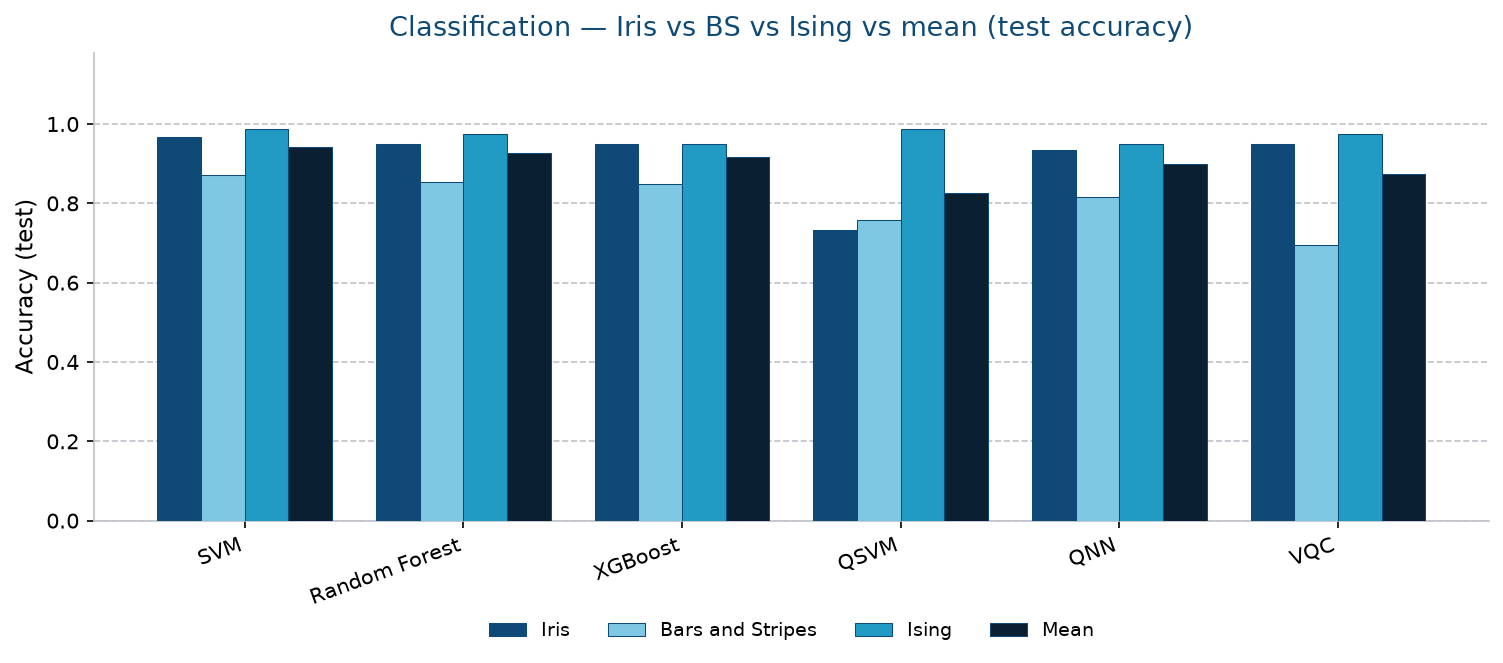
\includegraphics[width=0.95\textwidth]{cls_iris_vs_bs_vs_ising_vs_mean_accuracy.png}
\caption{Comparativa de exactitud del QSVC frente al mejor clasificador clásico en los tres datasets del Notebook~06 (una única partición por dataset). La ventaja de $+8.9$~pp sobre el dataset cuántico-nativo ($n=150$, 45 puntos de test) contrasta con la desventaja de $-4.0$~pp sobre SKG Incidentes y $-3.8$~pp sobre Telco Churn.}
\label{fig:quantum_kernel_3ds}
\end{figure}

\begin{figure}[htbp]
\centering
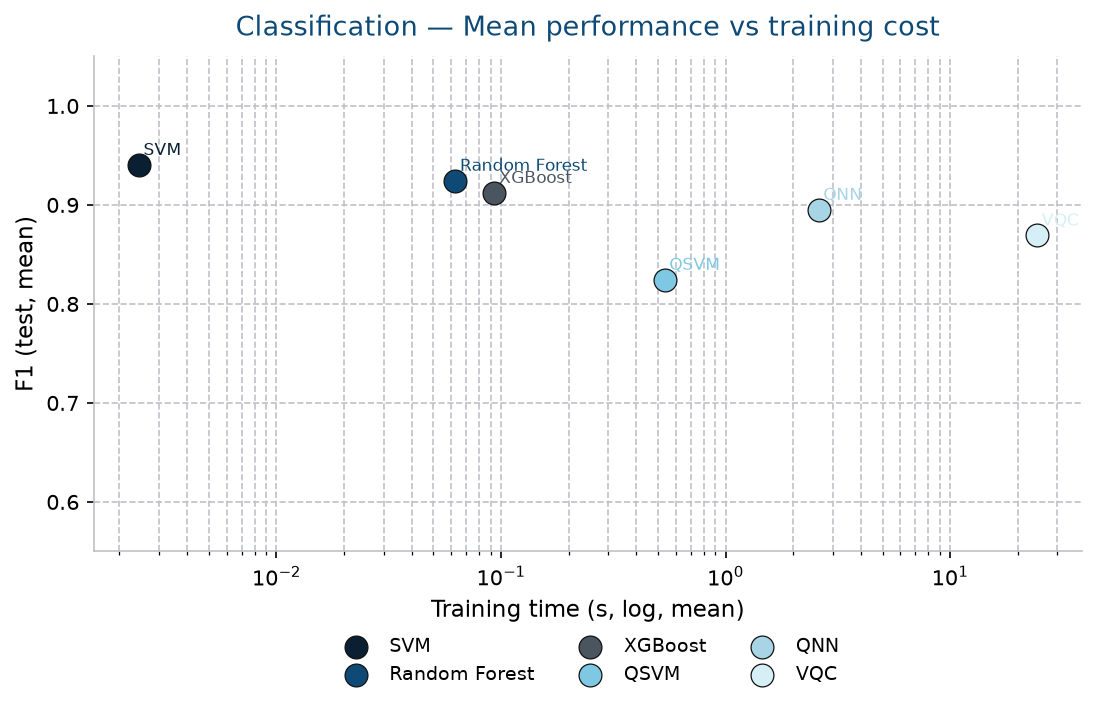
\includegraphics[width=0.90\textwidth]{cls_performance_vs_cost.png}
\caption{Exactitud del QSVM y del mejor clásico (Gradient Boosting) en el dataset cuántico-nativo según el número total de muestras ($n=50$ a $150$, 30\% de test) y diferencia entre ambos (Notebook~06). Cada barra procede de una única partición con 15 a 45 puntos de test (un acierto equivale a 2--7~pp): el QSVM queda por debajo de Gradient Boosting para $n=50$ y $80$ y por encima para $n\ge 100$. La repetición con 10 semillas (Tabla~\ref{tab:escala_clasificacion}) da una ventaja positiva en todos los tamaños, de modo que esta figura debe leerse como una realización ruidosa y no como un umbral de ventaja.}
\label{fig:kernel_escalabilidad}
\end{figure}

% =====================================================================
\section{Figuras complementarias: Notebook~07 — Síntesis visual de resultados}
\label{anx:figuras_nb07}
% =====================================================================

El dashboard comparativo (Figura~\ref{fig:dashboard_sintesis}) y el mapa de calor (Figura~\ref{fig:heatmap_ventaja_body}) se encuentran en el cuerpo del documento (Capítulo~5 y Capítulo~7). La siguiente figura complementa ese análisis con la comparativa de complejidad computacional teórica.

\begin{figure}[htbp]
\centering
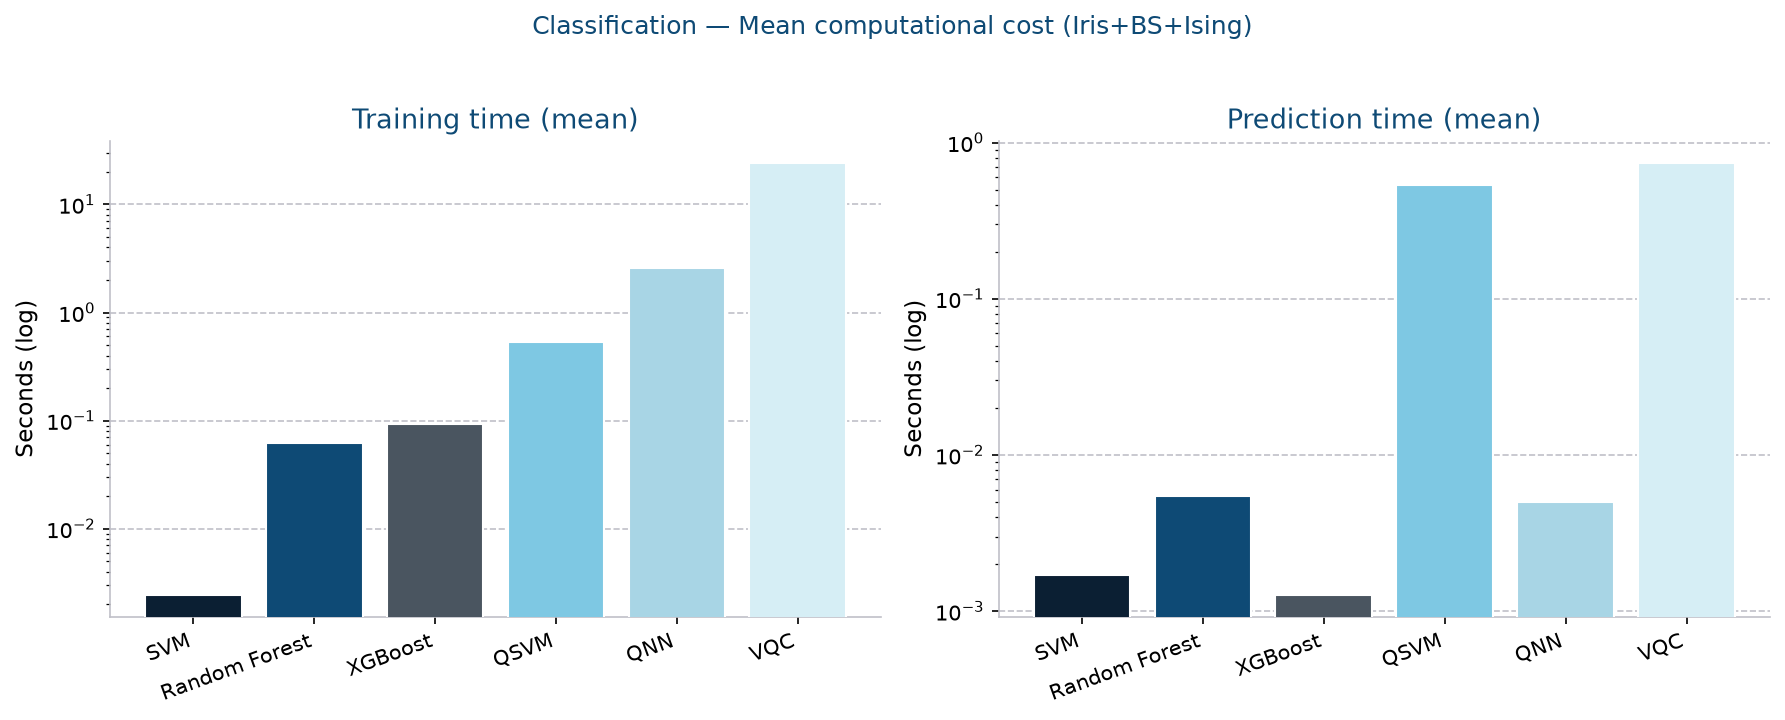
\includegraphics[width=0.90\textwidth]{cls_runtimes.png}
\caption{Comparativa de complejidad computacional teórica de los algoritmos cuánticos y sus contrapartes clásicas en cada caso de uso. Las barras muestran el orden de crecimiento ($O(\cdot)$) en función del tamaño del problema $n$. En los casos de optimización combinatoria (Casos~4, 5 y~7), la brecha de complejidad teórica justifica la exploración cuántica a escala (Notebook~07).}
\label{fig:complejidad_cuantico_clasico}
\end{figure}

% =====================================================================
\section{Figura complementaria: Notebook~09 — Barrido de rotaciones QCR}
\label{anx:figuras_nb0809}
% =====================================================================

El barrido sintético de cuanticidad (Figura~\ref{fig:barrido_sintetico_alpha}) y la correlación de indicadores (Figura~\ref{fig:correlacion_indicadores_body}) se encuentran en el Capítulo~\ref{cap:investigacion_original}. La siguiente figura complementa el análisis de la Estrategia~2 del Framework QCR.

\begin{figure}[htbp]
\centering
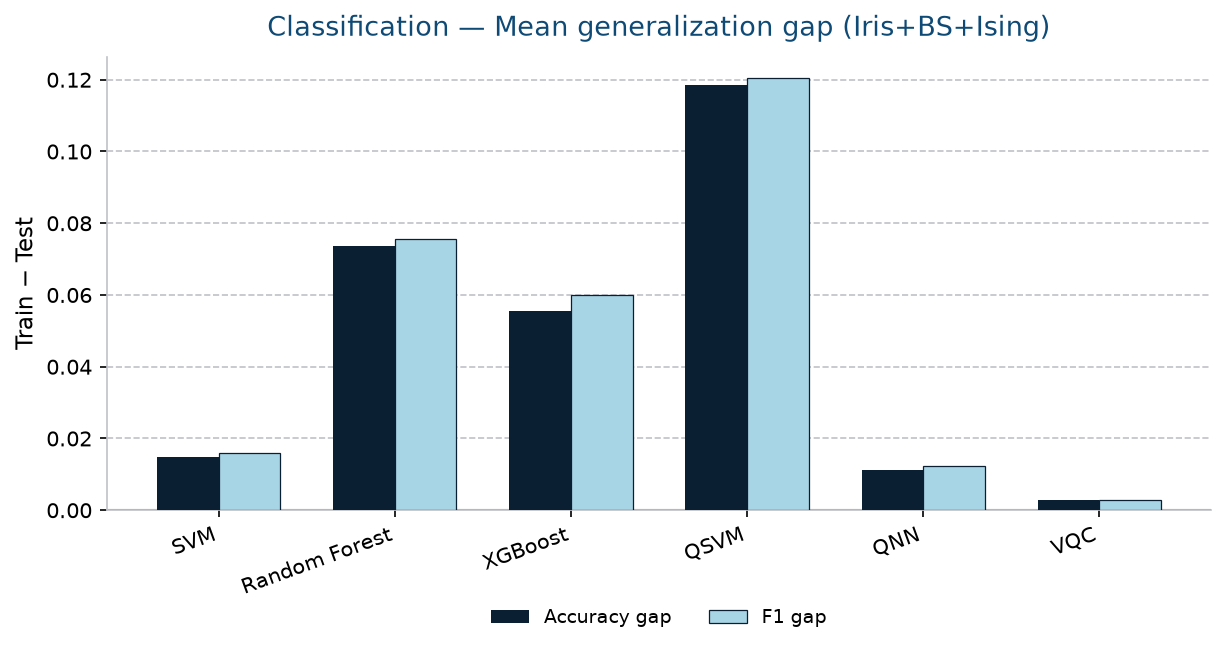
\includegraphics[width=0.90\textwidth]{cls_generalization_gap.png}
\caption{Barrido de la estrategia de rotación hacia máxima divergencia cuántico-clásica (Estrategia~2 del Framework QCR): variación de $d_F$, $\mathcal{Q}(\mathcal{D})$ y ventaja QSVM en función del ángulo de rotación $\theta \in [0, \pi/2]$ aplicado a SKG Incidentes y Telco Churn. La mejora de $d_F$ no se traduce consistentemente en ventaja empírica, confirmando la disociación entre capacidad teórica del kernel y rendimiento bajo muestras finitas (Notebook~09).}
\label{fig:barrido_rotaciones}
\end{figure}


\end{document}